\documentclass[]{book}
\usepackage{lmodern}
\usepackage{amssymb,amsmath}
\usepackage{ifxetex,ifluatex}
\usepackage{fixltx2e} % provides \textsubscript
\ifnum 0\ifxetex 1\fi\ifluatex 1\fi=0 % if pdftex
  \usepackage[T1]{fontenc}
  \usepackage[utf8]{inputenc}
\else % if luatex or xelatex
  \ifxetex
    \usepackage{mathspec}
  \else
    \usepackage{fontspec}
  \fi
  \defaultfontfeatures{Ligatures=TeX,Scale=MatchLowercase}
\fi
% use upquote if available, for straight quotes in verbatim environments
\IfFileExists{upquote.sty}{\usepackage{upquote}}{}
% use microtype if available
\IfFileExists{microtype.sty}{%
\usepackage{microtype}
\UseMicrotypeSet[protrusion]{basicmath} % disable protrusion for tt fonts
}{}
\usepackage[margin=1in]{geometry}
\usepackage{hyperref}
\hypersetup{unicode=true,
            pdftitle={Curso de Jurimetria},
            pdfauthor={Associação Brasileira de Jurimetria},
            pdfborder={0 0 0},
            breaklinks=true}
\urlstyle{same}  % don't use monospace font for urls
\usepackage{natbib}
\bibliographystyle{apalike}
\usepackage{color}
\usepackage{fancyvrb}
\newcommand{\VerbBar}{|}
\newcommand{\VERB}{\Verb[commandchars=\\\{\}]}
\DefineVerbatimEnvironment{Highlighting}{Verbatim}{commandchars=\\\{\}}
% Add ',fontsize=\small' for more characters per line
\usepackage{framed}
\definecolor{shadecolor}{RGB}{248,248,248}
\newenvironment{Shaded}{\begin{snugshade}}{\end{snugshade}}
\newcommand{\KeywordTok}[1]{\textcolor[rgb]{0.13,0.29,0.53}{\textbf{{#1}}}}
\newcommand{\DataTypeTok}[1]{\textcolor[rgb]{0.13,0.29,0.53}{{#1}}}
\newcommand{\DecValTok}[1]{\textcolor[rgb]{0.00,0.00,0.81}{{#1}}}
\newcommand{\BaseNTok}[1]{\textcolor[rgb]{0.00,0.00,0.81}{{#1}}}
\newcommand{\FloatTok}[1]{\textcolor[rgb]{0.00,0.00,0.81}{{#1}}}
\newcommand{\ConstantTok}[1]{\textcolor[rgb]{0.00,0.00,0.00}{{#1}}}
\newcommand{\CharTok}[1]{\textcolor[rgb]{0.31,0.60,0.02}{{#1}}}
\newcommand{\SpecialCharTok}[1]{\textcolor[rgb]{0.00,0.00,0.00}{{#1}}}
\newcommand{\StringTok}[1]{\textcolor[rgb]{0.31,0.60,0.02}{{#1}}}
\newcommand{\VerbatimStringTok}[1]{\textcolor[rgb]{0.31,0.60,0.02}{{#1}}}
\newcommand{\SpecialStringTok}[1]{\textcolor[rgb]{0.31,0.60,0.02}{{#1}}}
\newcommand{\ImportTok}[1]{{#1}}
\newcommand{\CommentTok}[1]{\textcolor[rgb]{0.56,0.35,0.01}{\textit{{#1}}}}
\newcommand{\DocumentationTok}[1]{\textcolor[rgb]{0.56,0.35,0.01}{\textbf{\textit{{#1}}}}}
\newcommand{\AnnotationTok}[1]{\textcolor[rgb]{0.56,0.35,0.01}{\textbf{\textit{{#1}}}}}
\newcommand{\CommentVarTok}[1]{\textcolor[rgb]{0.56,0.35,0.01}{\textbf{\textit{{#1}}}}}
\newcommand{\OtherTok}[1]{\textcolor[rgb]{0.56,0.35,0.01}{{#1}}}
\newcommand{\FunctionTok}[1]{\textcolor[rgb]{0.00,0.00,0.00}{{#1}}}
\newcommand{\VariableTok}[1]{\textcolor[rgb]{0.00,0.00,0.00}{{#1}}}
\newcommand{\ControlFlowTok}[1]{\textcolor[rgb]{0.13,0.29,0.53}{\textbf{{#1}}}}
\newcommand{\OperatorTok}[1]{\textcolor[rgb]{0.81,0.36,0.00}{\textbf{{#1}}}}
\newcommand{\BuiltInTok}[1]{{#1}}
\newcommand{\ExtensionTok}[1]{{#1}}
\newcommand{\PreprocessorTok}[1]{\textcolor[rgb]{0.56,0.35,0.01}{\textit{{#1}}}}
\newcommand{\AttributeTok}[1]{\textcolor[rgb]{0.77,0.63,0.00}{{#1}}}
\newcommand{\RegionMarkerTok}[1]{{#1}}
\newcommand{\InformationTok}[1]{\textcolor[rgb]{0.56,0.35,0.01}{\textbf{\textit{{#1}}}}}
\newcommand{\WarningTok}[1]{\textcolor[rgb]{0.56,0.35,0.01}{\textbf{\textit{{#1}}}}}
\newcommand{\AlertTok}[1]{\textcolor[rgb]{0.94,0.16,0.16}{{#1}}}
\newcommand{\ErrorTok}[1]{\textcolor[rgb]{0.64,0.00,0.00}{\textbf{{#1}}}}
\newcommand{\NormalTok}[1]{{#1}}
\usepackage{longtable,booktabs}
\usepackage{graphicx,grffile}
\makeatletter
\def\maxwidth{\ifdim\Gin@nat@width>\linewidth\linewidth\else\Gin@nat@width\fi}
\def\maxheight{\ifdim\Gin@nat@height>\textheight\textheight\else\Gin@nat@height\fi}
\makeatother
% Scale images if necessary, so that they will not overflow the page
% margins by default, and it is still possible to overwrite the defaults
% using explicit options in \includegraphics[width, height, ...]{}
\setkeys{Gin}{width=\maxwidth,height=\maxheight,keepaspectratio}
\IfFileExists{parskip.sty}{%
\usepackage{parskip}
}{% else
\setlength{\parindent}{0pt}
\setlength{\parskip}{6pt plus 2pt minus 1pt}
}
\setlength{\emergencystretch}{3em}  % prevent overfull lines
\providecommand{\tightlist}{%
  \setlength{\itemsep}{0pt}\setlength{\parskip}{0pt}}
\setcounter{secnumdepth}{5}
% Redefines (sub)paragraphs to behave more like sections
\ifx\paragraph\undefined\else
\let\oldparagraph\paragraph
\renewcommand{\paragraph}[1]{\oldparagraph{#1}\mbox{}}
\fi
\ifx\subparagraph\undefined\else
\let\oldsubparagraph\subparagraph
\renewcommand{\subparagraph}[1]{\oldsubparagraph{#1}\mbox{}}
\fi
\usepackage{booktabs}
\setlength\parindent{20pt}
\linespread{1.6}
\usepackage[scaled=.8]{beramono}
\renewcommand\arraystretch{0.7}
\renewcommand{\familydefault}{\sfdefault}

%%% Use protect on footnotes to avoid problems with footnotes in titles
\let\rmarkdownfootnote\footnote%
\def\footnote{\protect\rmarkdownfootnote}

%%% Change title format to be more compact
\usepackage{titling}

% Create subtitle command for use in maketitle
\newcommand{\subtitle}[1]{
  \posttitle{
    \begin{center}\large#1\end{center}
    }
}

\setlength{\droptitle}{-2em}
  \title{Curso de Jurimetria}
  \pretitle{\vspace{\droptitle}\centering\huge}
  \posttitle{\par}
  \author{Associação Brasileira de Jurimetria}
  \preauthor{\centering\large\emph}
  \postauthor{\par}
  \predate{\centering\large\emph}
  \postdate{\par}
  \date{2016-08-19}

\begin{document}
\maketitle

{
\setcounter{tocdepth}{1}
\tableofcontents
}
\chapter{Introdução}\label{introducao}

Essa é a primeira iteração do curso de Jurimetria da ABJ. Nesse curso
abordamos aspectos teóricos e práticos da Jurimetria, essenciais para um
profissional da Estatística que tenha interesse em trabalhar nessa área
de pesquisa.

O curso é voltado para estatísticos e está organizado em duas partes
principais. Na primeira parte, apresentamos as ferramentas de trabalho
do laboratório de Jurimetria, que permitem a execução de nossas
pesquisas. Na segunda parte, apresentamos diversas aplicações da
Jurimetria, focando em metodolodia de pesquisa, técnicas estatísticas e
conceitos fundamentais de Jurimetria.

Para a primeira parte do curso, será necessário ter conhecimentos do
software estatístico \texttt{R}, como a lógica de programação, sintaxe
do R e ambientação com o \texttt{RStudio}. Para as partes seguintes,
será necessário ter conhecimentos básicos de estatística, como
probabilidade, verossimilhança, inferência e processos estocásticos.

\section{Definição de Jurimetria}\label{definicao-de-jurimetria}

Podemos definir Jurimetria como a \emph{disciplina do conhecimento que
utiliza a metodologia estatística para investigar o funcionamento de uma
ordem jurídica}. A partir dela, fica claro que a Jurimetria se distingue
das demais disciplinas jurídicas, tanto pelo objeto como pela
metodologia empregada nas análises.

A Jurimetria tem três pilares operacionais: jurídico, estatístico e
computacional. É claro que a reunião dessas especialidades em uma só
pessoa é atualmente rara. Por isso, a prática da Jurimetria vem sendo
desenvolvida em um ambiente laboratorial em que bacharéis em direito,
estatísticos e cientistas da computação unem esforços na resolução de
problemas.

A Jurimetria propõe um giro epistemológico, análogo àquele proposto pelo
\emph{realismo jurídico}, deslocando o centro de interesse da pesquisa
do plano abstrato para o plano concreto. O conceito norteador deste giro
é que o direito efetivo, aquele capaz de afetar a relação entre
sujeitos, correspondente às sentenças, acórdãos, contratos e demais
ordens jurídicas produzidas no plano concreto.

A lei é uma declaração de intenções do legislador, que muitas vezes se
mostra plurívoca, contraditória e lacunosa. Para a jurimetria, é no
plano concreto que o Direito se revela, sendo a lei apenas um dos
fatores - ao lado dos valores pessoais, religião, empatia, experiência
pessoal de vida e outros tantos -, capaz de influenciar o processo de
concretização das normas do Direito. Por tal razão, o Direito não pode
ser reduzido a um conjunto de normas editado por autoridades competentes
e deve ser visto, sim, como um aparato de solução de conflitos, no qual
a lei desempenha um papel importante, porém não suficiente.

Estudar de forma concreta significa \textbf{situar o objeto de estudo no
tempo e no espaço}. Uma vantagem desse tipo de abordagem é que há
clareza na construção do escopo das pesquisas, o que pode levar a
conclusões mais diretas. Para tornar os estudos factíveis, no entanto,
também é necessário definir claramente o arcabouço de suposições no qual
as conclusões são válidas.

Utilizar a abordagem concreta não significa que pensar de forma abstrata
é ruim. Para construção de modelos capazes de mensurar certas
quantidades de forma adequada, ou para elaborar soluções para um
problema na lei, é necessário desconstruir o fenômeno de maneira ampla,
utilizar criatividade e intuição. A concretude ajuda ao direcionar as
abstrações e ligá-las a um objetivo pragmático.

A jurimetria também assume como ponto de partida a possibilidade modelar
certos fenômenos do direito como eventos aleatórios. Essa abordagem
contrasta com a abordagem clássica, que usa o determinismo fatalista
como realidade do direito. As vantagens em assumir aleatoriedade em
modelos jurimétricos confundem-se com as vantagens da utilização da
metodologia estatística em geral. Ao aceitar que há incerteza nos
modelos e que não somos em geral capazes de dar respostas definitivas às
nossas perguntas, ganhamos a habilidade de afirmar mais sobre o
desconhecido, associando possíveis resultados a suas respectivas
verossimilhanças.

Neste curso, abordaremos aplicações dentro dos tribunais, na
administração e para a sociedade. Após estudar este material, o
estatístico terá base suficiente para planejar e executar estudos
jurimétricos, que poderão auxiliar na elaboração de políticas públicas,
na gestão judiciária e administração de tribunais.

\chapter{Ferramental de trabalho da
ABJ}\label{ferramental-de-trabalho-da-abj}

As bases de dados utilizadas em estudos jurimétricos foram originalmente
concebidas para fins gerenciais e não analíticos. Por isso, observamos
muitos dados faltantes, mal formatados e com documentação inadequada.
Uma boa porção dos dados só está disponível em páginas HTML e arquivos
PDF e grande parte da informação útil está escondida em textos.

Chamamos esse fenômeno de ``pré-sal sociológico''. Temos hoje diversas
bases de dados armazenadas em repositórios públicos ou controladas pelo
poder público, mas que precisam ser lapidadas para obtenção de
informação útil.

O jurimetrista trabalha com dados sujos e desorganizados, mas gera muito
valor ao extrair suas informações. Por isso, o profissional precisa
dominar o ferramental\\
de extração, transformação e visualização de dados, e é sobre isso que
discutiremos nesta primeira parte do curso. Utilizaremos como base o
software estatístico \texttt{R}, que atualmente possui diversas
ferramentas que ajudam nessas atividades.

Os pacotes utilizados nessa parte são \texttt{httr}, \texttt{xml2},
\texttt{rvest}, \texttt{dplyr}, \texttt{tidyr}, \texttt{purrr},
\texttt{lubridate}, \texttt{stringr} e \texttt{ggplot2}. Também
utilizamos um pacote chamado \texttt{abjutils}, construído para atender
algumas necessidades frequentes da ABJ. Recomenda-se a utilização do
\texttt{R\ 3.3.1} e o \emph{RStudio preview version}\footnote{\href{https://www.rstudio.com/products/rstudio/download/preview/}{Baixe
  aqui}.}. É possível instalar todos esses pacotes de uma vez rodando

\begin{Shaded}
\begin{Highlighting}[]
\NormalTok{if (!}\KeywordTok{require}\NormalTok{(devtools)) }\KeywordTok{install.packages}\NormalTok{(}\StringTok{'devtools'}\NormalTok{)}
\NormalTok{devtools::}\KeywordTok{install_github}\NormalTok{(}\StringTok{'abjur/abjutils'}\NormalTok{)}
\end{Highlighting}
\end{Shaded}

\section{Exemplo trabalhado}\label{exemplo-trabalhado}

\subsection{Câmaras do TJSP}\label{camaras-do-tjsp}

Uma das principais questões que surgem quando o tema é impunidade e que
motivou esse trabalho é: quando um réu condenado deve começar a cumprir
pena? A justiça deve esperar o encerramento definitivo do processo, com
o chamado trânsito em julgado, ou pode iniciar o cumprimento já a partir
de uma decisão terminativa, como a sentença ou o acórdão de segundo
grau?

Uma forma de solucionar esse debate é calcular as taxas de reforma de
decisões em matéria criminal. Uma condição necessária para a viabilidade
da antecipação do cumprimento de pena é uma baixa taxa de reforma das
decisões, pois uma taxa alta implicaria que muitas pessoas seriam presas
injustamente.

Com o objetivo de obter essas taxas, a presente pesquisa utiliza como
base de dados um levantamento de 157.379 decisões em segunda instância,
das quais pouco menos de 60.000 envolvem apelações contra o Ministério
Público, todas proferidas entre 01/01/2014 e 31/12/2014 nas dezesseis
Câmaras de Direito Criminal, e nas quatro Câmaras Extraordinárias do
Tribunal de Justiça de São Paulo. Todas as informações foram obtidas
através de \emph{web scraping} a partir de bases de dados disponíveis
publicamente, o que permite a reprodutibilidade da pesquisa. Os dados
semi-estruturados foram organizados a partir da utilização de técnicas
de mineração de texto.

Os resultados revelam taxas de reforma próximas a 50\%. As taxas obtidas
são relevantes e justificam a não antecipação do cumprimento de pena
para a decisão em primeira instância.

Com o intuito de complementar e aprofundar a pesquisa, realizamos
análises para tipos específicos de crime, como roubo e tráfico de
drogas, comparando as taxas de reforma em cada subpopulação. Realizamos
também a comparação dos resultados relativamente às câmaras de
julgamento e relatores.

A partir dessa análise, observamos uma alta variabilidade na taxa de
reforma entre as vinte câmaras de julgamento. Encontramos câmaras com
mais de 75\% de recursos negados (quarta e sexta) e câmaras com menos de
30\% de recursos negados (primeira, segunda e décima segunda). O
resultado é contraintuitivo pois teoricamente a alocação de novos
recursos nas câmaras é aleatória.

No curso, vamos replicar o estudo das câmaras para 2015, passando por
todas as fases! Como são muitos processos, vamos trabalhar com uma
amostra de apenas mil casos para as visualizações finais.

\begin{Shaded}
\begin{Highlighting}[]
\KeywordTok{library}\NormalTok{(dplyr)}
\end{Highlighting}
\end{Shaded}

\begin{verbatim}
## 
## Attaching package: 'dplyr'
\end{verbatim}

\begin{verbatim}
## The following objects are masked from 'package:stats':
## 
##     filter, lag
\end{verbatim}

\begin{verbatim}
## The following objects are masked from 'package:base':
## 
##     intersect, setdiff, setequal, union
\end{verbatim}

\begin{Shaded}
\begin{Highlighting}[]
\NormalTok{d_cjsg <-}\StringTok{ }\KeywordTok{readRDS}\NormalTok{(}\StringTok{'data-raw/d_cjsg.rds'}\NormalTok{)}

\NormalTok{d_cjsg}
\end{Highlighting}
\end{Shaded}

\begin{verbatim}
## # A tibble: 184,250 x 14
##                                                      arq    id cd_acordao
##                                                    <chr> <chr>      <chr>
## 1  /home/storage/abj/raw/TJSP/cjsg/cjsg_mes01/00001.html     1    9381267
## 2  /home/storage/abj/raw/TJSP/cjsg/cjsg_mes01/00001.html     2    8671548
## 3  /home/storage/abj/raw/TJSP/cjsg/cjsg_mes01/00001.html     3    8634338
## 4  /home/storage/abj/raw/TJSP/cjsg/cjsg_mes01/00001.html     4    8536605
## 5  /home/storage/abj/raw/TJSP/cjsg/cjsg_mes01/00001.html     5    8509346
## 6  /home/storage/abj/raw/TJSP/cjsg/cjsg_mes01/00001.html     6    8490681
## 7  /home/storage/abj/raw/TJSP/cjsg/cjsg_mes01/00001.html     7    8466583
## 8  /home/storage/abj/raw/TJSP/cjsg/cjsg_mes01/00001.html     8    8449087
## 9  /home/storage/abj/raw/TJSP/cjsg/cjsg_mes01/00001.html     9    8429536
## 10 /home/storage/abj/raw/TJSP/cjsg/cjsg_mes01/00001.html    10    8331899
## # ... with 184,240 more rows, and 11 more variables: n_processo <chr>,
## #   comarca <chr>, data_julgamento <chr>, data_registro <chr>,
## #   ementa <chr>, orgao_julgador <chr>, outros_numeros <chr>,
## #   relatora <chr>, classe_assunto <chr>, txt_ementa <chr>, result <chr>
\end{verbatim}

\section{Data tidying}\label{data-tidying}

Uma base de dados é considerada ``tidy'' se

\begin{itemize}
\tightlist
\item
  Cada observação é uma linha do bd.
\item
  Cada variável é uma coluna do bd.
\item
  Para cada unidade observacional temos um \texttt{data\_frame} separado
  (possivelmente com chaves de associação).
\end{itemize}

Nessa parte do curso, vamos trabalhar com
\href{http://r4ds.had.co.nz/wrangle-intro.html}{\emph{arrumação de
dados}}, que consiste em trabalhar com ferramentas de extração,
consolidação e transformação de dados. As ferramentas utilizadas fazem
parte do chamado \texttt{tidyverse}, um universo de pacotes
contemporâneos do \texttt{R} que são intuitivos, eficientes e úteis.

O objetivo em \emph{arrumação de dados} é extrair e transformar uma base
de dados até que ela esteja em formato \emph{tidy}. Em seguida,
mostraremos como fizemos isso no exemplo das câmaras. Adicionalmente,
vamos apresentar como foram trabalhados os arquivos PDF no caso do Waze
do judiciário.

\section{Pipe}\label{pipe}

O operador \emph{pipe} foi uma das grandes revoluções recentes do R,
tornando a leitura de códigos mais lógica, fácil e compreensível. Este
operador foi introduzido por Stefan Milton Bache no pacote
\texttt{magrittr} e já existem diversos pacotes construidos para
facilitar a sua utilização.

Basicamente, o operador \texttt{\%\textgreater{}\%} usa o resultado do
seu lado esquerdo como primeiro argumento da função do lado direito. Só
isso!

Para usar o operador \texttt{\%\textgreater{}\%}, primeiramente devemos
instalar o pacote \texttt{magrittr}

\begin{Shaded}
\begin{Highlighting}[]
\KeywordTok{install.packages}\NormalTok{(}\StringTok{"magrittr"}\NormalTok{)}
\end{Highlighting}
\end{Shaded}

e carregá-lo com a função \texttt{library()}

\begin{Shaded}
\begin{Highlighting}[]
\KeywordTok{library}\NormalTok{(magrittr)}
\end{Highlighting}
\end{Shaded}

Feito isso, vamos testar o operador calculando a raiz quadrada da soma
de alguns números.

\begin{Shaded}
\begin{Highlighting}[]
\NormalTok{x <-}\StringTok{ }\KeywordTok{c}\NormalTok{(}\DecValTok{1}\NormalTok{, }\DecValTok{2}\NormalTok{, }\DecValTok{3}\NormalTok{, }\DecValTok{4}\NormalTok{)}
\NormalTok{x %>%}\StringTok{ }\NormalTok{sum %>%}\StringTok{ }\NormalTok{sqrt}
\end{Highlighting}
\end{Shaded}

\begin{verbatim}
## [1] 3.162278
\end{verbatim}

O caminho que o código acima seguiu foi enviar o objeto \texttt{x} como
argumento da função \texttt{sum()} e, em seguida, enviar a saida da
expressão \texttt{sum(x)} como argumento da função \texttt{sqrt()}.
Observe que não é necessário colocar os parênteses após o nome das
funções.

Se escrevermos esse cálculo na forma usual, temos o seguinte código:

\begin{Shaded}
\begin{Highlighting}[]
\KeywordTok{sqrt}\NormalTok{(}\KeywordTok{sum}\NormalTok{(x))}
\end{Highlighting}
\end{Shaded}

\begin{verbatim}
## [1] 3.162278
\end{verbatim}

A princípio, a utilização do \texttt{\%\textgreater{}\%} não parece
trazer grandes vantagens, pois a expressão \texttt{sqrt(sum(x))} é
facilmente compreendida. No entanto, se tivermos um grande número de
funções aninhadas, a utilização do \texttt{pipe} transforma um código
confuso e difícil de ser lido em algo simples e intuitivo. Como exemplo,
imagine que você precise escrever uma receita de um bolo usando o R, e
cada passo da receita é uma função:

\begin{Shaded}
\begin{Highlighting}[]
\KeywordTok{esfrie}\NormalTok{(}\KeywordTok{asse}\NormalTok{(}\KeywordTok{coloque}\NormalTok{(}\KeywordTok{bata}\NormalTok{(}\KeywordTok{acrescente}\NormalTok{(}\KeywordTok{recipiente}\NormalTok{(}\KeywordTok{rep}\NormalTok{(}\StringTok{"farinha"}\NormalTok{, }\DecValTok{2}\NormalTok{), }\StringTok{"água"}\NormalTok{, }\StringTok{"fermento"}\NormalTok{, }\StringTok{"leite"}\NormalTok{, }\StringTok{"óleo"}\NormalTok{), }\StringTok{"farinha"}\NormalTok{, até =}\StringTok{ "macio"}\NormalTok{), duraçã}\DataTypeTok{o =} \StringTok{"3min"}\NormalTok{), }\DataTypeTok{lugar =} \StringTok{"forma"}\NormalTok{, }\DataTypeTok{tipo =} \StringTok{"grande"}\NormalTok{, }\DataTypeTok{untada =} \NormalTok{T), duraçã}\DataTypeTok{o =} \StringTok{"50min"}\NormalTok{), }\StringTok{"geladeira"}\NormalTok{, }\StringTok{"20min"}\NormalTok{)}
\end{Highlighting}
\end{Shaded}

Tente entender o que é preciso fazer. Nada fácil, correto? Agora
escrevemos usando o operador \texttt{\%\textgreater{}\%}:

\begin{Shaded}
\begin{Highlighting}[]
\KeywordTok{recipiente}\NormalTok{(}\KeywordTok{rep}\NormalTok{(}\StringTok{"farinha"}\NormalTok{, }\DecValTok{2}\NormalTok{), }\StringTok{"água"}\NormalTok{, }\StringTok{"fermento"}\NormalTok{, }\StringTok{"leite"}\NormalTok{, }\StringTok{"óleo"}\NormalTok{) %>%}
\StringTok{  }\KeywordTok{acrescente}\NormalTok{(}\StringTok{"farinha"}\NormalTok{, até =}\StringTok{ "macio"}\NormalTok{) %>%}
\StringTok{  }\KeywordTok{bata}\NormalTok{(duraçã}\DataTypeTok{o =} \StringTok{"3min"}\NormalTok{) %>%}
\StringTok{  }\KeywordTok{coloque}\NormalTok{(}\DataTypeTok{lugar =} \StringTok{"forma"}\NormalTok{, }\DataTypeTok{tipo =} \StringTok{"grande"}\NormalTok{, }\DataTypeTok{untada =} \NormalTok{T) %>%}
\StringTok{  }\KeywordTok{asse}\NormalTok{(duraçã}\DataTypeTok{o =} \StringTok{"50min"}\NormalTok{) %>%}
\StringTok{  }\KeywordTok{esfrie}\NormalTok{(}\StringTok{"geladeira"}\NormalTok{, }\StringTok{"20min"}\NormalTok{)}
\end{Highlighting}
\end{Shaded}

Agora o código realmente se parece com uma receita de bolo.

Para mais informações sobre o \texttt{pipe} e exemplos de utilização,
visite a página
\href{http://cran.r-project.org/web/packages/magrittr/vignettes/magrittr.html}{Ceci
n'est pas un pipe}.

\section{\texorpdfstring{Pacote \texttt{lubridate} para trabalhar com
datas}{Pacote lubridate para trabalhar com datas}}\label{pacote-lubridate-para-trabalhar-com-datas}

Originalmente, o \texttt{R} é bastante ruim para trabalhar com datas, o
que causa frustração e perda de tempo nas análises. O pacote
\texttt{lubridate} foi criado para simplificar ao máximo a leitura de
datas e extração de informações dessas datas.

A função mais importante para leitura de dados no \texttt{lubridate} é a
\texttt{ymd}. Essa função serve para ler qualquer data de uma
\texttt{string} no formato \texttt{YYYY-MM-DD}. Essa função é útil pois
funciona com qualquer separador entre os elementos da data e também
porque temos uma função para cada formato (\texttt{mdy}, \texttt{dmy},
\texttt{dym}, \texttt{myd}, \texttt{ydm}).

\begin{Shaded}
\begin{Highlighting}[]
\NormalTok{d1 <-}\StringTok{ '04/15/06'}
\KeywordTok{library}\NormalTok{(lubridate)}
\end{Highlighting}
\end{Shaded}

\begin{verbatim}
## 
## Attaching package: 'lubridate'
\end{verbatim}

\begin{verbatim}
## The following object is masked from 'package:base':
## 
##     date
\end{verbatim}

Outras funções importantes

\begin{itemize}
\tightlist
\item
  \texttt{ymd\_hms}: lê datas e horários, generalizando \texttt{ymd}.
\item
  \texttt{year}, \texttt{month}, \texttt{day}, \texttt{quarter},
  \texttt{weekday}, \texttt{week}: extraem componentes da data.
\item
  \texttt{years}, \texttt{months}, \texttt{days}: adicionam tempos a uma
  data, ajudando a criar vetores de datas. Por exemplo
\end{itemize}

\begin{Shaded}
\begin{Highlighting}[]
\KeywordTok{library}\NormalTok{(lubridate)}
\KeywordTok{ymd}\NormalTok{(}\StringTok{'2015-01-01'}\NormalTok{) +}\StringTok{ }\KeywordTok{months}\NormalTok{(}\DecValTok{0}\NormalTok{:}\DecValTok{11}\NormalTok{)}
\end{Highlighting}
\end{Shaded}

\begin{verbatim}
##  [1] "2015-01-01" "2015-02-01" "2015-03-01" "2015-04-01" "2015-05-01"
##  [6] "2015-06-01" "2015-07-01" "2015-08-01" "2015-09-01" "2015-10-01"
## [11] "2015-11-01" "2015-12-01"
\end{verbatim}

\begin{itemize}
\tightlist
\item
  \texttt{floor\_date} e \texttt{ceiling\_date}: arredonda datas para
  uma unidade de interesse. Útil para agregar dados diários por semana,
  mês, trimestre etc.
\end{itemize}

Mais informações: ver
\href{https://cran.r-project.org/web/packages/lubridate/vignettes/lubridate.html}{aqui}
e
\href{https://www.jstatsoft.org/index.php/jss/article/view/v040i03/v40i03.pdf}{aqui}.

\section{\texorpdfstring{Pacote \texttt{stringr} para trabalhar com
textos}{Pacote stringr para trabalhar com textos}}\label{pacote-stringr-para-trabalhar-com-textos}

O R básico não tem uma sintaxe consistente para trabalhar com textos. O
pacote \texttt{stringr} ajuda a realizar todas as tarefas básicas de
manipulação de texto, exigindo que o usuário estude apenas uma sintaxe.
O \texttt{stringr} também é construído sobre a
\href{http://site.icu-project.org/}{biblioteca ICU}, implementada em
\texttt{C} e \texttt{C++}, apresentando resultados rápidos e confiáveis.

As regras básicas do pacote são:

\begin{itemize}
\tightlist
\item
  As funções de manipulação de texto começam com \texttt{str\_}. Caso
  esqueça o nome de uma função, basta digitar \texttt{stringr::str\_} e
  apertar \texttt{TAB} para ver quais são as opções.
\item
  O primeiro argumento da função é sempre uma \texttt{string}.
\end{itemize}

Antes de listar as funções, precisamos estudar o básico de expressões
regulares.

\subsection{Expressões regulares}\label{expressoes-regulares}

Expressão regular ou \emph{regex} é uma sequência concisa de caracteres
que representa várias strings. Entender o básico de expressões regulares
é indispensável para trabalhar com textos.

Vamos estudar expressões regulares através de exemplos e com a função
\texttt{str\_detect()}. Essa função retorna \texttt{TRUE} se uma string
atende à uma expressão regular e \texttt{FALSE} em caso contrário.

A tabela abaixo mostra a aplicação de seis \texttt{regex} a seis strings
distintas.

\begin{Shaded}
\begin{Highlighting}[]
\KeywordTok{library}\NormalTok{(stringr)}
\NormalTok{testes <-}\StringTok{ }\KeywordTok{c}\NormalTok{(}\StringTok{'ban'}\NormalTok{, }\StringTok{'banana'}\NormalTok{, }\StringTok{'abandonado'}\NormalTok{, }\StringTok{'pranab anderson'}\NormalTok{, }\StringTok{'BANANA'}\NormalTok{, }\StringTok{'ele levou ban'}\NormalTok{)}

\NormalTok{expressoes <-}\StringTok{ }\KeywordTok{list}\NormalTok{(}
  \StringTok{'ban'}\NormalTok{, }\CommentTok{# reconhece tudo que tenha "ban", mas não ignora case}
  \StringTok{'BAN'}\NormalTok{, }\CommentTok{# reconhece tudo que tenha "BAN", mas não ignora case}
  \KeywordTok{regex}\NormalTok{(}\StringTok{'ban'}\NormalTok{, }\DataTypeTok{ignore_case =} \OtherTok{TRUE}\NormalTok{), }\CommentTok{# reconhece tudo que tenha "ban", ignorando case}
  \StringTok{'ban$'}\NormalTok{, }\CommentTok{# reconhece apenas o que termina exatamente em "ban"}
  \StringTok{'^ban'}\NormalTok{, }\CommentTok{# reconhece apenas o que começa exatamente com "ban"}
  \StringTok{'b ?an'} \CommentTok{# reconhece tudo que tenha "ban", com ou sem espaço entre o "b" e o "a"}
\NormalTok{)}
\end{Highlighting}
\end{Shaded}

\begin{tabular}{l|l|l|l|l|l|l}
\hline
regex & ban & banana & abandonado & pranab anderson & BANANA & ele levou ban\\
\hline
ban & TRUE & TRUE & TRUE & FALSE & FALSE & TRUE\\
\hline
BAN & FALSE & TRUE & FALSE & FALSE & FALSE & FALSE\\
\hline
ban & FALSE & FALSE & TRUE & FALSE & FALSE & FALSE\\
\hline
ban\$ & FALSE & FALSE & FALSE & TRUE & FALSE & FALSE\\
\hline
\textasciicircum{}ban & FALSE & FALSE & FALSE & FALSE & TRUE & FALSE\\
\hline
b ?an & FALSE & FALSE & FALSE & FALSE & FALSE & TRUE\\
\hline
\end{tabular}

\subsubsection{Quantificadores}\label{quantificadores}

Os caracteres \texttt{+}, \texttt{*} e \texttt{\{x,y\}} indicam quantas
vezes um padrão se repete:

\begin{itemize}
\tightlist
\item
  \texttt{ey+} significa \texttt{e} e depois \texttt{y} ``\textbf{uma
  vez} ou mais''. Por exemplo, reconhece \texttt{hey}, \texttt{heyy},
  \texttt{a\ eyyy}, mas não reconhece \texttt{e}, \texttt{y} nem
  \texttt{yy}.
\item
  \texttt{ey*} significa ``\textbf{zero vezes} ou mais''. Por exemplo,
  reconhece \texttt{hey}, \texttt{heyy}, \texttt{a\ eyyy} e \texttt{e},
  mas não reconhece \texttt{y} nem \texttt{yy}.
\item
  \texttt{ey\{3\}} significa ``exatamente três vezes''. Por exemplo,
  reconhece \texttt{eyyy} e \texttt{eyyyy}, mas não reconhece
  \texttt{eyy}.
\item
  \texttt{ey\{1,3\}} significa ``entre uma e três vezes''.
\end{itemize}

Para aplicar um quantificador a um conjunto de caracteres, use
parênteses. Por exemplo, \texttt{(ey\ )+} reconhece \texttt{ey\ ey}.

\subsubsection{Conjuntos}\label{conjuntos}

Colocando caracteres dentro de \texttt{{[}{]}}, reconhecemos quaisquer
caracteres desse conjunto. Alguns exemplos práticos:

\begin{itemize}
\tightlist
\item
  \texttt{{[}Cc{]}asa} para reconhecer ``casa'' em maiúsculo ou
  minúsculo.
\item
  \texttt{{[}0-9{]}} para reconhecer somente números. O mesmo vale para
  letras \texttt{{[}a-z{]}}, \texttt{{[}A-Z{]}}, \texttt{{[}a-zA-Z{]}}
  etc.
\item
  O símbolo \texttt{\^{}} dentro do colchete significa negação. Por
  exemplo, \texttt{{[}\^{}0-9{]}} significa pegar tudo o que não é
  número.
\item
  O símbolo \texttt{.} fora do colchete indica ``qualquer caractere'',
  mas dentro do colchete é apenas ponto.
\item
  Use \texttt{{[}{[}:space:{]}{]}+} para reconhecer espaços e
  \texttt{{[}{[}:punct:{]}{]}+} para reconhecer pontuações.
\end{itemize}

\subsubsection{Miscelânea}\label{miscelanea}

\begin{itemize}
\tightlist
\item
  Use \texttt{abjutils::rm\_accent()} para retirar os acentos de um
  texto.
\item
  Use \texttt{\textbar{}} para opções, por exemplo
  \texttt{desfavor\textbar{}desprov} reconhece tanto ``desfavorável''
  quanto ``desprovido''
\item
  \texttt{\textbackslash{}n} pula linha, \texttt{\textbackslash{}f} é
  final da página, \texttt{\textbackslash{}t} é tab. Use
  \texttt{\textbackslash{}} para transformar caracteres especiais em
  literais.
\item
  \texttt{tolower()} e \texttt{toupper()} para mudar o case de uma
  string.
\end{itemize}

A lista de possibilidades com expressões regulares é extensa. Um bom
lugar para testar o funcionamento de expressões regulares é o
\href{https://regex101.com/}{regex101}.

\subsection{\texorpdfstring{Funções do
\texttt{stringr}}{Funções do stringr}}\label{funcoes-do-stringr}

\begin{itemize}
\item
  \texttt{str\_detect()} retorna \texttt{TRUE} se a regex é compatível
  com a string e \texttt{FALSE} caso contrário
\item
  \texttt{str\_lengh()} retorna o comprimento de uma string.
\end{itemize}

\begin{Shaded}
\begin{Highlighting}[]
\KeywordTok{str_length}\NormalTok{(}\StringTok{'hye'}\NormalTok{)}
\end{Highlighting}
\end{Shaded}

\begin{verbatim}
## [1] 3
\end{verbatim}

\begin{itemize}
\tightlist
\item
  \texttt{str\_trim()} retira espaços e quebras de linha/tabs no início
  ou final de string.
\end{itemize}

\begin{Shaded}
\begin{Highlighting}[]
\NormalTok{string <-}\StringTok{ '}\CharTok{\textbackslash{}n}\StringTok{essa      string é muito suja       }\CharTok{\textbackslash{}n}\StringTok{'}
\KeywordTok{str_trim}\NormalTok{(string)}
\end{Highlighting}
\end{Shaded}

\begin{verbatim}
## [1] "essa      string é muito suja"
\end{verbatim}

\begin{itemize}
\tightlist
\item
  \texttt{str\_replace()} e \texttt{str\_replace\_all()} substituem um
  padrão (ou todos) encontrado para um outro padrão
\end{itemize}

\begin{Shaded}
\begin{Highlighting}[]
\NormalTok{string <-}\StringTok{ 'heyyy ui yy'}
\KeywordTok{str_replace}\NormalTok{(string, }\StringTok{'y'}\NormalTok{, }\StringTok{'x'}\NormalTok{)}
\end{Highlighting}
\end{Shaded}

\begin{verbatim}
## [1] "hexyy ui yy"
\end{verbatim}

\begin{Shaded}
\begin{Highlighting}[]
\KeywordTok{str_replace}\NormalTok{(string, }\StringTok{'y+'}\NormalTok{, }\StringTok{'x'}\NormalTok{)}
\end{Highlighting}
\end{Shaded}

\begin{verbatim}
## [1] "hex ui yy"
\end{verbatim}

\begin{Shaded}
\begin{Highlighting}[]
\KeywordTok{str_replace_all}\NormalTok{(string, }\StringTok{'y'}\NormalTok{, }\StringTok{'x'}\NormalTok{)}
\end{Highlighting}
\end{Shaded}

\begin{verbatim}
## [1] "hexxx ui xx"
\end{verbatim}

\begin{Shaded}
\begin{Highlighting}[]
\KeywordTok{str_replace_all}\NormalTok{(}\StringTok{'string     com    muitos espaços'}\NormalTok{, }\StringTok{' +'}\NormalTok{, }\StringTok{' '}\NormalTok{) }\CommentTok{# tirar espaços extras}
\end{Highlighting}
\end{Shaded}

\begin{verbatim}
## [1] "string com muitos espaços"
\end{verbatim}

\begin{itemize}
\tightlist
\item
  \texttt{str\_match()} e \texttt{str\_match\_all()} extrai pedaços da
  string identificados pela regex. Caso queira extrair somente a parte
  identificada, use parênteses.
\end{itemize}

\begin{Shaded}
\begin{Highlighting}[]
\NormalTok{frases <-}\StringTok{ }\KeywordTok{c}\NormalTok{(}\StringTok{'a roupa do rei'}\NormalTok{, }\StringTok{'de roma'}\NormalTok{, }\StringTok{'o rato roeu'}\NormalTok{)}
\KeywordTok{str_match}\NormalTok{(frases, }\StringTok{'roe'}\NormalTok{)}
\end{Highlighting}
\end{Shaded}

\begin{verbatim}
##      [,1] 
## [1,] NA   
## [2,] NA   
## [3,] "roe"
\end{verbatim}

\begin{Shaded}
\begin{Highlighting}[]
\KeywordTok{str_match_all}\NormalTok{(frases, }\StringTok{'ro'}\NormalTok{)}
\end{Highlighting}
\end{Shaded}

\begin{verbatim}
## [[1]]
##      [,1]
## [1,] "ro"
## 
## [[2]]
##      [,1]
## [1,] "ro"
## 
## [[3]]
##      [,1]
## [1,] "ro"
\end{verbatim}

\begin{Shaded}
\begin{Highlighting}[]
\KeywordTok{str_match}\NormalTok{(frases, }\StringTok{'o (ro)'}\NormalTok{)}
\end{Highlighting}
\end{Shaded}

\begin{verbatim}
##      [,1]   [,2]
## [1,] NA     NA  
## [2,] NA     NA  
## [3,] "o ro" "ro"
\end{verbatim}

\begin{itemize}
\tightlist
\item
  \texttt{str\_split()} separa uma string em várias de acordo com um
  separador.
\end{itemize}

\begin{Shaded}
\begin{Highlighting}[]
\NormalTok{string <-}\StringTok{ 'eu sei, usar virgulas, de forma, perfeita'}

\KeywordTok{str_split}\NormalTok{(string, }\StringTok{', '}\NormalTok{)}
\end{Highlighting}
\end{Shaded}

\begin{verbatim}
## [[1]]
## [1] "eu sei"        "usar virgulas" "de forma"      "perfeita"
\end{verbatim}

\begin{Shaded}
\begin{Highlighting}[]
\KeywordTok{str_split}\NormalTok{(string, }\StringTok{', '}\NormalTok{, }\DataTypeTok{simplify =} \OtherTok{TRUE}\NormalTok{)}
\end{Highlighting}
\end{Shaded}

\begin{verbatim}
##      [,1]     [,2]            [,3]       [,4]      
## [1,] "eu sei" "usar virgulas" "de forma" "perfeita"
\end{verbatim}

\begin{itemize}
\tightlist
\item
  \texttt{str\_split\_fixed()} faz o mesmo que \texttt{str\_split()},
  mas separa apenas \texttt{n} vezes
\end{itemize}

\begin{Shaded}
\begin{Highlighting}[]
\KeywordTok{str_split_fixed}\NormalTok{(string, }\StringTok{', '}\NormalTok{, }\DecValTok{3}\NormalTok{)}
\end{Highlighting}
\end{Shaded}

\begin{verbatim}
##      [,1]     [,2]            [,3]                
## [1,] "eu sei" "usar virgulas" "de forma, perfeita"
\end{verbatim}

\begin{Shaded}
\begin{Highlighting}[]
\KeywordTok{str_split_fixed}\NormalTok{(string, }\StringTok{', '}\NormalTok{, }\DecValTok{4}\NormalTok{) }\CommentTok{# igual a str_split(string, simplify = TRUE)}
\end{Highlighting}
\end{Shaded}

\begin{verbatim}
##      [,1]     [,2]            [,3]       [,4]      
## [1,] "eu sei" "usar virgulas" "de forma" "perfeita"
\end{verbatim}

\begin{itemize}
\tightlist
\item
  \texttt{str\_sub()} extrai uma parte da string de acordo com os
  índices.
\end{itemize}

\begin{Shaded}
\begin{Highlighting}[]
\NormalTok{string <-}\StringTok{ 'quero pegar só uma parte disso'}
\KeywordTok{str_sub}\NormalTok{(string, }\DecValTok{13}\NormalTok{, }\DecValTok{14}\NormalTok{)}
\end{Highlighting}
\end{Shaded}

\begin{verbatim}
## [1] "só"
\end{verbatim}

\begin{Shaded}
\begin{Highlighting}[]
\KeywordTok{str_sub}\NormalTok{(string, -}\DecValTok{5}\NormalTok{, -}\DecValTok{1}\NormalTok{) }\CommentTok{# usar números negativos para voltar do final da string}
\end{Highlighting}
\end{Shaded}

\begin{verbatim}
## [1] "disso"
\end{verbatim}

\begin{Shaded}
\begin{Highlighting}[]
\NormalTok{indices <-}\StringTok{ }\KeywordTok{str_locate}\NormalTok{(string, }\StringTok{'parte'}\NormalTok{)}
\NormalTok{indices}
\end{Highlighting}
\end{Shaded}

\begin{verbatim}
##      start end
## [1,]    20  24
\end{verbatim}

\begin{Shaded}
\begin{Highlighting}[]
\KeywordTok{str_sub}\NormalTok{(string, indices) }\CommentTok{# pode ser útil usar com str_locate.}
\end{Highlighting}
\end{Shaded}

\begin{verbatim}
## [1] "parte"
\end{verbatim}

\begin{itemize}
\tightlist
\item
  \texttt{str\_subset()} retorna somente as strings compatíveis com a
  regex.
\end{itemize}

\begin{Shaded}
\begin{Highlighting}[]
\NormalTok{frases <-}\StringTok{ }\KeywordTok{c}\NormalTok{(}\StringTok{'a roupa do rei'}\NormalTok{, }\StringTok{'de roma'}\NormalTok{, }\StringTok{'o rato roeu'}\NormalTok{)}
\KeywordTok{str_subset}\NormalTok{(frases, }\StringTok{'d[eo]'}\NormalTok{)}
\end{Highlighting}
\end{Shaded}

\begin{verbatim}
## [1] "a roupa do rei" "de roma"
\end{verbatim}

\subsection{Exemplo: decisões das
câmaras}\label{exemplo-decisoes-das-camaras}

Suponha que temos o seguinte vetor de textos de decisões:

\begin{Shaded}
\begin{Highlighting}[]
\NormalTok{d_decisoes <-}\StringTok{ }\KeywordTok{readRDS}\NormalTok{(}\StringTok{'data-raw/d_decisoes.rds'}\NormalTok{)}

\NormalTok{condicao <-}\StringTok{ }\KeywordTok{str_length}\NormalTok{(d_decisoes$decisao) <}\StringTok{ }\DecValTok{200} \NormalTok{&}\StringTok{ }\NormalTok{d_decisoes$situacao ==}\StringTok{ 'Julgado'}
\KeywordTok{set.seed}\NormalTok{(}\DecValTok{1247}\NormalTok{) }\CommentTok{# reprodutibilidade}
\NormalTok{decisoes <-}\StringTok{ }\NormalTok{d_decisoes$decisao[condicao] %>%}\StringTok{ }\KeywordTok{sample}\NormalTok{(}\DecValTok{10}\NormalTok{, }\DataTypeTok{replace =} \OtherTok{FALSE}\NormalTok{)}
\NormalTok{decisoes}
\end{Highlighting}
\end{Shaded}

\begin{verbatim}
##  [1] "Negaram provimento ao recurso. V. U."                                                                                           
##  [2] "NEGARAM PROVIMENTO ao recurso. V.U."                                                                                            
##  [3] "Negaram provimento ao apelo do réu.V.U."                                                                                        
##  [4] "Deram provimento ao apelo ministerial para anular o julgamento pelo Tribunal do Júri, devendo a outro ser submetido o réu. V.U."
##  [5] "Declararam prejudicado o exame do recurso.V.U."                                                                                 
##  [6] "DERAM PROVIMENTO PARCIAL ao recurso para corrigir a pena de multa para 87 dias-multa, mantida, no mais, a r. sentença. V.U."    
##  [7] "Rejeitaram as preliminares arguidas e negaram provimento à apelação. V.U."                                                      
##  [8] "Negaram provimento ao recurso. V. U."                                                                                           
##  [9] "Negaram provimento ao recurso. V. U."                                                                                           
## [10] "Negaram provimento aos recursos defensivos e deram provimento ao recurso ministerial nos termos do V. Acórdão. V.U."
\end{verbatim}

\begin{Shaded}
\begin{Highlighting}[]
\NormalTok{negaram <-}\StringTok{ }\KeywordTok{regex}\NormalTok{(}\StringTok{'negaram'}\NormalTok{, }\DataTypeTok{ignore_case =} \OtherTok{TRUE}\NormalTok{)}
\NormalTok{parcial <-}\StringTok{ }\KeywordTok{regex}\NormalTok{(}\StringTok{'parcial'}\NormalTok{, }\DataTypeTok{ignore_case =} \OtherTok{TRUE}\NormalTok{)}
\NormalTok{deram <-}\StringTok{ }\KeywordTok{regex}\NormalTok{(}\StringTok{'deram'}\NormalTok{, }\DataTypeTok{ignore_case =} \OtherTok{TRUE}\NormalTok{)}

\NormalTok{tipos_decisao <-}\StringTok{ }\NormalTok{function(decisoes) \{}
  \KeywordTok{ifelse}\NormalTok{(}
    \KeywordTok{str_detect}\NormalTok{(decisoes, negaram), }\StringTok{'negado'}\NormalTok{, }\KeywordTok{ifelse}\NormalTok{(}
      \KeywordTok{str_detect}\NormalTok{(decisoes, parcial), }\StringTok{'parcial'}\NormalTok{, }\KeywordTok{ifelse}\NormalTok{(}
        \KeywordTok{str_detect}\NormalTok{(decisoes, deram), }\StringTok{'provido'}\NormalTok{, }\StringTok{'outros'}
    \NormalTok{))}
  \NormalTok{)}
\NormalTok{\}}
\end{Highlighting}
\end{Shaded}

Resultados:

\begin{Shaded}
\begin{Highlighting}[]
\NormalTok{tibble::}\KeywordTok{tibble}\NormalTok{(}\DataTypeTok{tipo_decisao =} \KeywordTok{tipos_decisao}\NormalTok{(decisoes), }\DataTypeTok{decisao =} \NormalTok{decisoes_min)}
\end{Highlighting}
\end{Shaded}

\begin{verbatim}
## # A tibble: 10 x 2
##    tipo_decisao                                            decisao
##           <chr>                                              <chr>
## 1        negado               Negaram provimento ao recurso. V. U.
## 2        negado                NEGARAM PROVIMENTO ao recurso. V.U.
## 3        negado            Negaram provimento ao apelo do réu.V.U.
## 4       provido Deram provimento ao apelo ministerial para anul...
## 5        outros     Declararam prejudicado o exame do recurso.V.U.
## 6       parcial DERAM PROVIMENTO PARCIAL ao recurso para corrig...
## 7        negado Rejeitaram as preliminares arguidas e negaram p...
## 8        negado               Negaram provimento ao recurso. V. U.
## 9        negado               Negaram provimento ao recurso. V. U.
## 10       negado Negaram provimento aos recursos defensivos e de...
\end{verbatim}

\section{\texorpdfstring{Pacotes \texttt{dplyr} e
\texttt{tidyr}}{Pacotes dplyr e tidyr}}\label{pacotes-dplyr-e-tidyr}

A transformação de dados é uma tarefa usualmente dolorosa e demorada,
podendo tomar a maior parte do tempo da análise. No entanto, como nosso
interesse geralmente é na modelagem dos dados, essa tarefa é muitas
vezes negligenciada.

O \texttt{dplyr} é um dos pacotes mais úteis para realizar manipulação
de dados, e procura aliar simplicidade e eficiência de uma forma
bastante elegante. Os scripts em \texttt{R} que fazem uso inteligente
dos verbos \texttt{dplyr} e as facilidades do operador \emph{pipe}
tendem a ficar mais legíveis e organizados, sem perder velocidade de
execução.

\begin{quote}
``(\ldots{}) The fact that data science exists as a field is a colossal
failure of statistics. To me, {[}what I do{]} is what statistics is all
about. It is gaining insight from data using modelling and
visualization. Data munging and manipulation is hard and statistics has
just said that's not our domain.''

Hadley Wickham
\end{quote}

Por ser um pacote que se propõe a realizar um dos trabalhos mais árduos
da análise estatística, e por atingir esse objetivo de forma elegante,
eficaz e eficiente, o \texttt{dplyr} pode ser considerado como uma
revolução no \texttt{R}.

\subsection{\texorpdfstring{Trabalhando com
\texttt{tibble}s}{Trabalhando com tibbles}}\label{trabalhando-com-tibbles}

A \texttt{tibble} nada mais é do que um \texttt{data.frame}, mas com um
método de impressão mais adequado. Outras diferenças podem ser estudadas
\href{http://r4ds.had.co.nz/tibbles.html}{neste link}.

Vamos assumir que temos a seguinte base de dados:

\begin{Shaded}
\begin{Highlighting}[]
\NormalTok{d_cjsg}
\end{Highlighting}
\end{Shaded}

\begin{verbatim}
## # A tibble: 184,250 x 14
##                                                      arq    id cd_acordao
##                                                    <chr> <chr>      <chr>
## 1  /home/storage/abj/raw/TJSP/cjsg/cjsg_mes01/00001.html     1    9381267
## 2  /home/storage/abj/raw/TJSP/cjsg/cjsg_mes01/00001.html     2    8671548
## 3  /home/storage/abj/raw/TJSP/cjsg/cjsg_mes01/00001.html     3    8634338
## 4  /home/storage/abj/raw/TJSP/cjsg/cjsg_mes01/00001.html     4    8536605
## 5  /home/storage/abj/raw/TJSP/cjsg/cjsg_mes01/00001.html     5    8509346
## 6  /home/storage/abj/raw/TJSP/cjsg/cjsg_mes01/00001.html     6    8490681
## 7  /home/storage/abj/raw/TJSP/cjsg/cjsg_mes01/00001.html     7    8466583
## 8  /home/storage/abj/raw/TJSP/cjsg/cjsg_mes01/00001.html     8    8449087
## 9  /home/storage/abj/raw/TJSP/cjsg/cjsg_mes01/00001.html     9    8429536
## 10 /home/storage/abj/raw/TJSP/cjsg/cjsg_mes01/00001.html    10    8331899
## # ... with 184,240 more rows, and 11 more variables: n_processo <chr>,
## #   comarca <chr>, data_julgamento <chr>, data_registro <chr>,
## #   ementa <chr>, orgao_julgador <chr>, outros_numeros <chr>,
## #   relatora <chr>, classe_assunto <chr>, txt_ementa <chr>, result <chr>
\end{verbatim}

\subsection{\texorpdfstring{As cinco funções principais do
\texttt{dplyr}}{As cinco funções principais do dplyr}}\label{as-cinco-funcoes-principais-do-dplyr}

\begin{itemize}
\tightlist
\item
  \texttt{filter}
\item
  \texttt{mutate}
\item
  \texttt{select}
\item
  \texttt{arrange}
\item
  \texttt{summarise}
\end{itemize}

\subsection{Características}\label{caracteristicas}

\begin{itemize}
\tightlist
\item
  O \emph{input} é sempre uma \texttt{tibble}, e o \emph{output} é
  sempre um \texttt{tibble}.
\item
  No primeiro argumento colocamos o \texttt{tibble}, e nos outros
  argumentos colocamo o que queremos fazer.
\item
  A utilização é facilitada com o emprego do operador
  \texttt{\%\textgreater{}\%}
\end{itemize}

\subsection{Vantagens}\label{vantagens}

\begin{itemize}
\tightlist
\item
  Utiliza \texttt{C} e \texttt{C++} por trás da maioria das funções, o
  que geralmente torna o código mais eficiente.
\item
  Pode trabalhar com diferentes fontes de dados, como bases relacionais
  (SQL) e \texttt{data.table}.
\end{itemize}

\subsection{\texorpdfstring{\texttt{select}}{select}}\label{select}

\begin{itemize}
\tightlist
\item
  Utilizar \texttt{starts\_with(x)}, \texttt{contains(x)},
  \texttt{matches(x)}, \texttt{one\_of(x)}, etc.
\item
  Possível colocar nomes, índices, e intervalos de variáveis com
  \texttt{:}.
\end{itemize}

\begin{Shaded}
\begin{Highlighting}[]
\NormalTok{d_cjsg %>%}\StringTok{ }
\StringTok{  }\KeywordTok{select}\NormalTok{(id, cd_acordao, comarca, }\DataTypeTok{relator =} \NormalTok{relatora)}
\end{Highlighting}
\end{Shaded}

\begin{verbatim}
## # A tibble: 184,250 x 4
##       id cd_acordao             comarca                  relator
##    <chr>      <chr>               <chr>                    <chr>
## 1      1    9381267           São Paulo           Encinas Manfré
## 2      2    8671548           Guarulhos           Edison Brandão
## 3      3    8634338              Osasco             Ivan Sartori
## 4      4    8536605          Adamantina          Walter da Silva
## 5      5    8509346             Limeira Guilherme de Souza Nucci
## 6      6    8490681           São Paulo         Roberto Solimene
## 7      7    8466583              Suzano             Poças Leitão
## 8      8    8449087 Presidente Prudente             Ivan Sartori
## 9      9    8429536           São Paulo           Willian Campos
## 10    10    8331899           São Paulo     Luis Soares de Mello
## # ... with 184,240 more rows
\end{verbatim}

\begin{Shaded}
\begin{Highlighting}[]
\NormalTok{d_cjsg %>%}\StringTok{ }
\StringTok{  }\KeywordTok{select}\NormalTok{(cd_acordao:comarca, classe_assunto)}
\end{Highlighting}
\end{Shaded}

\begin{verbatim}
## # A tibble: 184,250 x 4
##    cd_acordao                n_processo             comarca
##         <chr>                     <chr>               <chr>
## 1     9381267 0081568-68.2012.8.26.0050           São Paulo
## 2     8671548 2132739-15.2014.8.26.0000           Guarulhos
## 3     8634338 2204759-04.2014.8.26.0000              Osasco
## 4     8536605 2179832-71.2014.8.26.0000          Adamantina
## 5     8509346 2055376-49.2014.8.26.0000             Limeira
## 6     8490681 0014476-05.2014.8.26.0050           São Paulo
## 7     8466583 0067859-48.2014.8.26.0000              Suzano
## 8     8449087 0054802-60.2014.8.26.0000 Presidente Prudente
## 9     8429536 2128810-71.2014.8.26.0000           São Paulo
## 10    8331899 2002343-13.2015.8.26.0000           São Paulo
## # ... with 184,240 more rows, and 1 more variables: classe_assunto <chr>
\end{verbatim}

\begin{Shaded}
\begin{Highlighting}[]
\NormalTok{d_cjsg %>%}\StringTok{ }
\StringTok{  }\KeywordTok{select}\NormalTok{(n_processo, }\KeywordTok{starts_with}\NormalTok{(}\StringTok{'data_'}\NormalTok{))}
\end{Highlighting}
\end{Shaded}

\begin{verbatim}
## # A tibble: 184,250 x 3
##                   n_processo data_julgamento data_registro
##                        <chr>           <chr>         <chr>
## 1  0081568-68.2012.8.26.0050      29/01/2015    27/04/2016
## 2  2132739-15.2014.8.26.0000      27/01/2015    04/08/2015
## 3  2204759-04.2014.8.26.0000      27/01/2015    22/07/2015
## 4  2179832-71.2014.8.26.0000      22/01/2015    16/06/2015
## 5  2055376-49.2014.8.26.0000      27/01/2015    02/06/2015
## 6  0014476-05.2014.8.26.0050      29/01/2015    27/05/2015
## 7  0067859-48.2014.8.26.0000      29/01/2015    19/05/2015
## 8  0054802-60.2014.8.26.0000      27/01/2015    13/05/2015
## 9  2128810-71.2014.8.26.0000      29/01/2015    06/05/2015
## 10 2002343-13.2015.8.26.0000      27/01/2015    29/03/2015
## # ... with 184,240 more rows
\end{verbatim}

\subsection{\texorpdfstring{\texttt{filter}}{filter}}\label{filter}

\begin{itemize}
\tightlist
\item
  Parecido com \texttt{subset}.
\item
  Condições separadas por vírgulas é o mesmo que separar por
  \texttt{\&}.
\end{itemize}

\begin{Shaded}
\begin{Highlighting}[]
\NormalTok{d_cjsg %>%}\StringTok{ }
\StringTok{  }\KeywordTok{select}\NormalTok{(id, cd_acordao, comarca, }\DataTypeTok{relator =} \NormalTok{relatora) %>%}\StringTok{ }
\StringTok{  }\KeywordTok{filter}\NormalTok{(comarca ==}\StringTok{ 'São Paulo'}\NormalTok{)}
\end{Highlighting}
\end{Shaded}

\begin{verbatim}
## # A tibble: 41,488 x 4
##       id cd_acordao   comarca               relator
##    <chr>      <chr>     <chr>                 <chr>
## 1      1    9381267 São Paulo        Encinas Manfré
## 2      6    8490681 São Paulo      Roberto Solimene
## 3      9    8429536 São Paulo        Willian Campos
## 4     10    8331899 São Paulo  Luis Soares de Mello
## 5     12    8317638 São Paulo Sérgio Mazina Martins
## 6     13    8314983 São Paulo         Péricles Piza
## 7     14    8314866 São Paulo         Péricles Piza
## 8     17    8293299 São Paulo        Ivo de Almeida
## 9     19    8284691 São Paulo        Edison Brandão
## 10    21    8274010 São Paulo  Cesar Mecchi Morales
## # ... with 41,478 more rows
\end{verbatim}

\begin{Shaded}
\begin{Highlighting}[]
\KeywordTok{library}\NormalTok{(lubridate)}
\NormalTok{d_cjsg %>%}\StringTok{ }
\StringTok{  }\KeywordTok{select}\NormalTok{(id, cd_acordao, comarca, data_julgamento, }\DataTypeTok{relator =} \NormalTok{relatora) %>%}\StringTok{ }
\StringTok{  }\KeywordTok{filter}\NormalTok{(comarca %in%}\StringTok{ }\KeywordTok{c}\NormalTok{(}\StringTok{'Campinas'}\NormalTok{, }\StringTok{'Sorocaba'}\NormalTok{) &}
\StringTok{         }\NormalTok{(}\KeywordTok{day}\NormalTok{(}\KeywordTok{dmy}\NormalTok{(data_julgamento)) >=}\StringTok{ }\DecValTok{29} \NormalTok{|}\StringTok{ }\KeywordTok{day}\NormalTok{(}\KeywordTok{dmy}\NormalTok{(data_julgamento)) <}\StringTok{ }\DecValTok{25}\NormalTok{))}
\end{Highlighting}
\end{Shaded}

\begin{verbatim}
## # A tibble: 6,262 x 5
##       id cd_acordao  comarca data_julgamento                relator
##    <chr>      <chr>    <chr>           <chr>                  <chr>
## 1     33    8221266 Sorocaba      29/01/2015 Alcides Malossi Junior
## 2    136    8211543 Campinas      29/01/2015        Walter da Silva
## 3    174    8211235 Sorocaba      22/01/2015        Walter da Silva
## 4    188    8211081 Sorocaba      29/01/2015        Walter da Silva
## 5    190    8211053 Campinas      29/01/2015        Walter da Silva
## 6    229    8206214 Sorocaba      29/01/2015      Ricardo Tucunduva
## 7    312    8194316 Sorocaba      29/01/2015           Poças Leitão
## 8    354    8193920 Campinas      29/01/2015           Sérgio Ribas
## 9    417    8193329 Campinas      29/01/2015           Poças Leitão
## 10   427    8193274 Sorocaba      29/01/2015           Poças Leitão
## # ... with 6,252 more rows
\end{verbatim}

\begin{Shaded}
\begin{Highlighting}[]
\NormalTok{d_cjsg %>%}\StringTok{ }
\StringTok{  }\KeywordTok{select}\NormalTok{(comarca) %>%}\StringTok{ }
\StringTok{  }\KeywordTok{filter}\NormalTok{(}\KeywordTok{str_detect}\NormalTok{(comarca, }\StringTok{'^[gG]'}\NormalTok{))}
\end{Highlighting}
\end{Shaded}

\begin{verbatim}
## # A tibble: 6,463 x 1
##      comarca
##        <chr>
## 1  Guarulhos
## 2  Guarulhos
## 3  Guarulhos
## 4  Guarulhos
## 5      Guará
## 6  Guarulhos
## 7  Guarulhos
## 8  Guarulhos
## 9  Guarulhos
## 10 Guarulhos
## # ... with 6,453 more rows
\end{verbatim}

\subsection{\texorpdfstring{\texttt{mutate}}{mutate}}\label{mutate}

\begin{itemize}
\tightlist
\item
  Parecido com \texttt{transform}, mas aceita várias novas colunas
  iterativamente.
\item
  Novas variáveis devem ter o mesmo \texttt{length} que o \texttt{nrow}
  do bd oridinal ou \texttt{1}.
\end{itemize}

\begin{Shaded}
\begin{Highlighting}[]
\KeywordTok{library}\NormalTok{(stringr)}
\NormalTok{d_cjsg %>%}\StringTok{ }
\StringTok{  }\KeywordTok{select}\NormalTok{(id, n_processo, data_julgamento) %>%}\StringTok{ }
\StringTok{  }\KeywordTok{mutate}\NormalTok{(}\DataTypeTok{ano_julgamento =} \KeywordTok{year}\NormalTok{(}\KeywordTok{dmy}\NormalTok{(data_julgamento)),}
         \DataTypeTok{ano_proc =} \KeywordTok{str_sub}\NormalTok{(n_processo, }\DecValTok{12}\NormalTok{, }\DecValTok{15}\NormalTok{),}
         \DataTypeTok{ano_proc =} \KeywordTok{as.numeric}\NormalTok{(ano_proc),}
         \DataTypeTok{tempo_anos =} \NormalTok{ano_julgamento -}\StringTok{ }\NormalTok{ano_proc)}
\end{Highlighting}
\end{Shaded}

\begin{verbatim}
## # A tibble: 184,250 x 6
##       id                n_processo data_julgamento ano_julgamento ano_proc
##    <chr>                     <chr>           <chr>          <dbl>    <dbl>
## 1      1 0081568-68.2012.8.26.0050      29/01/2015           2015     2012
## 2      2 2132739-15.2014.8.26.0000      27/01/2015           2015     2014
## 3      3 2204759-04.2014.8.26.0000      27/01/2015           2015     2014
## 4      4 2179832-71.2014.8.26.0000      22/01/2015           2015     2014
## 5      5 2055376-49.2014.8.26.0000      27/01/2015           2015     2014
## 6      6 0014476-05.2014.8.26.0050      29/01/2015           2015     2014
## 7      7 0067859-48.2014.8.26.0000      29/01/2015           2015     2014
## 8      8 0054802-60.2014.8.26.0000      27/01/2015           2015     2014
## 9      9 2128810-71.2014.8.26.0000      29/01/2015           2015     2014
## 10    10 2002343-13.2015.8.26.0000      27/01/2015           2015     2015
## # ... with 184,240 more rows, and 1 more variables: tempo_anos <dbl>
\end{verbatim}

\subsection{\texorpdfstring{\texttt{arrange}}{arrange}}\label{arrange}

\begin{itemize}
\tightlist
\item
  Simplesmente ordena de acordo com as opções.
\item
  Utilizar \texttt{desc} para ordem decrescente.
\end{itemize}

\begin{Shaded}
\begin{Highlighting}[]
\KeywordTok{library}\NormalTok{(stringr)}
\NormalTok{d_cjsg %>%}\StringTok{ }
\StringTok{  }\KeywordTok{select}\NormalTok{(id, n_processo, data_julgamento) %>%}\StringTok{ }
\StringTok{  }\KeywordTok{mutate}\NormalTok{(}\DataTypeTok{ano_julgamento =} \KeywordTok{year}\NormalTok{(}\KeywordTok{dmy}\NormalTok{(data_julgamento)),}
         \DataTypeTok{ano_proc =} \KeywordTok{str_sub}\NormalTok{(n_processo, }\DecValTok{12}\NormalTok{, }\DecValTok{15}\NormalTok{),}
         \DataTypeTok{ano_proc =} \KeywordTok{as.numeric}\NormalTok{(ano_proc)) %>%}\StringTok{ }
\StringTok{  }\KeywordTok{mutate}\NormalTok{(}\DataTypeTok{tempo_anos =} \NormalTok{ano_julgamento -}\StringTok{ }\NormalTok{ano_proc) %>%}\StringTok{ }
\StringTok{  }\KeywordTok{arrange}\NormalTok{(}\KeywordTok{desc}\NormalTok{(tempo_anos))}
\end{Highlighting}
\end{Shaded}

\begin{verbatim}
## # A tibble: 184,250 x 6
##       id                n_processo data_julgamento ano_julgamento ano_proc
##    <chr>                     <chr>           <chr>          <dbl>    <dbl>
## 1   1797 0901097-67.1957.8.26.0050      30/04/2015           2015     1957
## 2  13650 0815784-50.1971.8.26.0050      12/11/2015           2015     1971
## 3   7222 9000001-18.1976.8.26.0309      16/07/2015           2015     1976
## 4   8228 9000001-74.1979.8.26.0224      23/02/2015           2015     1979
## 5   6512 0909882-46.1979.8.26.0050      26/05/2015           2015     1979
## 6   3439 9000001-81.1981.8.26.0005      26/02/2015           2015     1981
## 7   1469 0000014-17.1982.8.26.0292      29/01/2015           2015     1982
## 8  12850 0000784-59.1982.8.26.0114      02/07/2015           2015     1982
## 9   7040 0000019-02.1983.8.26.0584      27/01/2015           2015     1983
## 10  3920 2050003-20.1984.8.26.0281      26/02/2015           2015     1984
## # ... with 184,240 more rows, and 1 more variables: tempo_anos <dbl>
\end{verbatim}

\subsection{\texorpdfstring{\texttt{summarise}}{summarise}}\label{summarise}

\begin{itemize}
\tightlist
\item
  Retorna um vetor de tamanho \texttt{1} a partir de uma conta com as
  variáveis.
\item
  Geralmente é utilizado em conjunto com \texttt{group\_by}.
\item
  Algumas funções importantes: \texttt{n()}, \texttt{n\_distinct()}.
\end{itemize}

\begin{Shaded}
\begin{Highlighting}[]
\NormalTok{d_cjsg %>%}\StringTok{ }
\StringTok{  }\KeywordTok{select}\NormalTok{(id, n_processo, comarca, data_julgamento, orgao_julgador) %>%}\StringTok{ }
\StringTok{  }\KeywordTok{mutate}\NormalTok{(}\DataTypeTok{ano_julgamento =} \KeywordTok{year}\NormalTok{(}\KeywordTok{dmy}\NormalTok{(data_julgamento)),}
         \DataTypeTok{ano_proc =} \KeywordTok{str_sub}\NormalTok{(n_processo, }\DecValTok{12}\NormalTok{, }\DecValTok{15}\NormalTok{),}
         \DataTypeTok{ano_proc =} \KeywordTok{as.numeric}\NormalTok{(ano_proc)) %>%}\StringTok{ }
\StringTok{  }\KeywordTok{mutate}\NormalTok{(}\DataTypeTok{tempo_anos =} \NormalTok{ano_julgamento -}\StringTok{ }\NormalTok{ano_proc) %>%}\StringTok{ }
\StringTok{  }\KeywordTok{arrange}\NormalTok{(}\KeywordTok{desc}\NormalTok{(tempo_anos)) %>%}\StringTok{ }
\StringTok{  }\KeywordTok{group_by}\NormalTok{(comarca, orgao_julgador) %>%}\StringTok{ }
\StringTok{  }\KeywordTok{summarise}\NormalTok{(}\DataTypeTok{n =} \KeywordTok{n}\NormalTok{(),}
            \DataTypeTok{media_anos =} \KeywordTok{mean}\NormalTok{(tempo_anos),}
            \DataTypeTok{min_anos =} \KeywordTok{min}\NormalTok{(tempo_anos),}
            \DataTypeTok{max_anos =} \KeywordTok{max}\NormalTok{(tempo_anos)) %>%}\StringTok{ }
\StringTok{  }\KeywordTok{filter}\NormalTok{(n >}\StringTok{ }\DecValTok{5}\NormalTok{) %>%}\StringTok{ }
\StringTok{  }\KeywordTok{arrange}\NormalTok{(}\KeywordTok{desc}\NormalTok{(media_anos))}
\end{Highlighting}
\end{Shaded}

\begin{verbatim}
## Source: local data frame [4,351 x 6]
## Groups: comarca [271]
## 
##                  comarca                    orgao_julgador     n
##                    <chr>                             <chr> <int>
## 1                 Piraju 2ª Câmara Criminal Extraordinária     8
## 2         José Bonifácio 6ª Câmara Criminal Extraordinária     6
## 3           Miguelópolis 2ª Câmara Criminal Extraordinária     6
## 4                Piedade 3ª Câmara Criminal Extraordinária     6
## 5               Valinhos 1ª Câmara Criminal Extraordinária     6
## 6       Lençóis Paulista     2ª Câmara de Direito Criminal     8
## 7        Pindamonhangaba 5ª Câmara Criminal Extraordinária     8
## 8           Praia Grande 6ª Câmara Criminal Extraordinária     8
## 9  Santa Bárbara D Oeste 4ª Câmara Criminal Extraordinária     7
## 10             Ituverava 3ª Câmara Criminal Extraordinária     6
## # ... with 4,341 more rows, and 3 more variables: media_anos <dbl>,
## #   min_anos <dbl>, max_anos <dbl>
\end{verbatim}

\begin{Shaded}
\begin{Highlighting}[]
\NormalTok{d_cjsg %>%}\StringTok{ }
\StringTok{  }\KeywordTok{count}\NormalTok{(relatora, }\DataTypeTok{sort =} \OtherTok{TRUE}\NormalTok{) %>%}\StringTok{ }
\StringTok{  }\KeywordTok{mutate}\NormalTok{(}\DataTypeTok{prop =} \NormalTok{n /}\StringTok{ }\KeywordTok{sum}\NormalTok{(n), }\DataTypeTok{prop =} \NormalTok{scales::}\KeywordTok{percent}\NormalTok{(prop))}
\end{Highlighting}
\end{Shaded}

\begin{verbatim}
## # A tibble: 111 x 3
##                    relatora     n  prop
##                       <chr> <int> <chr>
## 1             Sérgio Coelho  3424 1.86%
## 2    Miguel Marques e Silva  3352 1.82%
## 3              Poças Leitão  2859 1.55%
## 4           Walter da Silva  2834 1.54%
## 5           Francisco Bruno  2767 1.50%
## 6            Edison Brandão  2748 1.49%
## 7                Souza Nery  2739 1.49%
## 8              Carlos Bueno  2730 1.48%
## 9            Ivo de Almeida  2661 1.44%
## 10 Guilherme de Souza Nucci  2639 1.43%
## # ... with 101 more rows
\end{verbatim}

\subsection{\texorpdfstring{\texttt{gather}}{gather}}\label{gather}

\begin{itemize}
\tightlist
\item
  ``Empilha'' o banco de dados
\end{itemize}

\begin{Shaded}
\begin{Highlighting}[]
\KeywordTok{library}\NormalTok{(tidyr)}
\NormalTok{d_cjsg %>%}\StringTok{ }
\StringTok{  }\KeywordTok{select}\NormalTok{(cd_acordao:data_registro) %>%}\StringTok{ }
\StringTok{  }\KeywordTok{gather}\NormalTok{(key, value, -cd_acordao) %>%}\StringTok{ }
\StringTok{  }\KeywordTok{arrange}\NormalTok{(cd_acordao)}
\end{Highlighting}
\end{Shaded}

\begin{verbatim}
## # A tibble: 737,000 x 3
##    cd_acordao             key                     value
##         <chr>           <chr>                     <chr>
## 1     8137574      n_processo 0209050-18.2013.8.26.0000
## 2     8137574         comarca                 São Paulo
## 3     8137574 data_julgamento                22/01/2015
## 4     8137574   data_registro                22/01/2015
## 5     8137600      n_processo 0016319-58.2014.8.26.0000
## 6     8137600         comarca                 São Paulo
## 7     8137600 data_julgamento                22/01/2015
## 8     8137600   data_registro                22/01/2015
## 9     8137628      n_processo 0104838-68.2005.8.26.0050
## 10    8137628         comarca                 São Paulo
## # ... with 736,990 more rows
\end{verbatim}

\subsection{\texorpdfstring{\texttt{spread}}{spread}}\label{spread}

\begin{itemize}
\tightlist
\item
  ``Joga'' uma variável nas colunas
\item
  É essencialmente a função inversa de \texttt{gather}
\end{itemize}

\begin{Shaded}
\begin{Highlighting}[]
\NormalTok{d_cjsg %>%}\StringTok{ }
\StringTok{  }\KeywordTok{distinct}\NormalTok{(cd_acordao, }\DataTypeTok{.keep_all =} \OtherTok{TRUE}\NormalTok{) %>%}\StringTok{ }
\StringTok{  }\KeywordTok{select}\NormalTok{(cd_acordao:data_registro) %>%}\StringTok{ }
\StringTok{  }\KeywordTok{gather}\NormalTok{(key, value, -cd_acordao) %>%}\StringTok{ }
\StringTok{  }\KeywordTok{spread}\NormalTok{(key, value)}
\end{Highlighting}
\end{Shaded}

\begin{verbatim}
## # A tibble: 184,249 x 5
##    cd_acordao                  comarca data_julgamento data_registro
## *       <chr>                    <chr>           <chr>         <chr>
## 1     8137574                São Paulo      22/01/2015    22/01/2015
## 2     8137600                São Paulo      22/01/2015    22/01/2015
## 3     8137628                São Paulo      22/01/2015    22/01/2015
## 4     8137638                São Paulo      22/01/2015    22/01/2015
## 5     8137663 Espírito Santo do Pinhal      22/01/2015    22/01/2015
## 6     8137671     Presidente Venceslau      22/01/2015    22/01/2015
## 7     8137677       Paraguaçu Paulista      22/01/2015    22/01/2015
## 8     8137690                Guarulhos      22/01/2015    22/01/2015
## 9     8137695                   Osasco      22/01/2015    22/01/2015
## 10    8137696                Americana      22/01/2015    22/01/2015
## # ... with 184,239 more rows, and 1 more variables: n_processo <chr>
\end{verbatim}

\subsection{Funções auxiliares}\label{funcoes-auxiliares}

\begin{itemize}
\tightlist
\item
  \texttt{unite} junta duas ou mais colunas usando algum separador
  (\texttt{\_}, por exemplo).
\item
  \texttt{separate} faz o inverso de \texttt{unite}, e uma coluna em
  várias usando um separador.
\end{itemize}

\begin{Shaded}
\begin{Highlighting}[]
\NormalTok{d_cjsg %>%}\StringTok{ }
\StringTok{  }\KeywordTok{select}\NormalTok{(n_processo, classe_assunto) %>%}\StringTok{ }
\StringTok{  }\KeywordTok{separate}\NormalTok{(classe_assunto, }\KeywordTok{c}\NormalTok{(}\StringTok{'classe'}\NormalTok{, }\StringTok{'assunto'}\NormalTok{), }\DataTypeTok{sep =} \StringTok{' / '}\NormalTok{, }
           \DataTypeTok{extra =} \StringTok{'merge'}\NormalTok{, }\DataTypeTok{fill =} \StringTok{'right'}\NormalTok{) %>%}\StringTok{ }
\StringTok{  }\KeywordTok{count}\NormalTok{(assunto, }\DataTypeTok{sort =} \OtherTok{TRUE}\NormalTok{)}
\end{Highlighting}
\end{Shaded}

\begin{verbatim}
## # A tibble: 287 x 2
##                                               assunto     n
##                                                 <chr> <int>
## 1                  Tráfico de Drogas e Condutas Afins 30993
## 2                                               Roubo 17556
## 3                                      Roubo Majorado 17461
## 4  Crimes de Tráfico Ilícito e Uso Indevido de Drogas 13635
## 5                                   Furto Qualificado 13275
## 6                         Pena Privativa de Liberdade 10801
## 7                                               Furto  9870
## 8                                Progressão de Regime  7068
## 9                                          Receptação  5978
## 10                Crimes do Sistema Nacional de Armas  5675
## # ... with 277 more rows
\end{verbatim}

\subsection{Um pouco mais de transformação de
dados}\label{um-pouco-mais-de-transformacao-de-dados}

\begin{itemize}
\tightlist
\item
  Para juntar tabelas, usar \texttt{inner\_join}, \texttt{left\_join},
  \texttt{anti\_join}, etc.
\item
  Para realizar operações mais gerais, usar \texttt{do}.
\item
  Para retirar duplicatas, utilizar \texttt{distinct}.
\end{itemize}

\section{\texorpdfstring{Pacotes \texttt{httr}, \texttt{xml2} e
\texttt{rvest}}{Pacotes httr, xml2 e rvest}}\label{pacotes-httr-xml2-e-rvest}

Esses são os três pacotes mais modernos do R utilizados para fazer web
scraping. O pacote \texttt{xml2} tem a finalidade de estruturar arquivos
HTML ou XML de forma eficiente, tornando possível a obtenção de
\emph{tags} e seus atributos dentro de um arquivo. Já o pacote
\texttt{httr} é responsável por realizar requisições web para obtenção
das páginas de interesse, buscando reduzir ao máximo a complexidade da
programação. O pacote \texttt{rvest} é escrito \textbf{sobre} os dois
anteriores e por isso eleva ainda mais o nível de especialização para
raspagem de dados.

As características dos pacotes implicam na seguinte regra de bolso. Para
trabalhar com páginas simples, basta carregar o \texttt{rvest} e
utilizar suas funcionalidades. Caso o acesso à página exija ações mais
complexas e/ou artifícios de ferramentas web, será necessário utilizar o
\texttt{httr}. O \texttt{xml2} só será usado explicitamente nos casos
raros em que a página está em XML, que pode ser visto como uma
generalização do HTML.

Esses pacotes não são suficientes para acessar todo tipo de conteúdo da
web. Um exemplo claro disso são páginas em que o conteúdo é produzido
por \texttt{javascript}, o que acontece em muitos sites modernos. Para
trabalhar com esses sites, é necessário realmente ``simular'' um
navegador que acessa a página web. Uma das melhores ferramentas para
isso é o \texttt{selenium}. Não discutiremos \texttt{selenium} nesse
curso, mas caso queira se aprofundar, acesse
\href{http://www.seleniumhq.org/}{aqui}.

\subsection{Sessões e cookies}\label{sessoes-e-cookies}

No momento que acessamos uma página web, nosso navegador baixa alguns
arquivos que ``identificam'' nosso acesso à página. Esses arquivos são
chamados cookies e são usados pelos sites para realizar diversas
atividades, como carregar uma página pré-definida pelo usuário caso este
acesse o site pela segunda vez.

O \texttt{httr} e por consequência o \texttt{rvest} já guardam esses
cookies de forma automática, de forma que o usuário não precise se
preocupar com isso. Em casos raros, para construir o web scraper é
necessário modificar esses cookies. Nesses casos, estude a função
\texttt{cookies()} do \texttt{httr}.

\subsection{\texorpdfstring{\texttt{GET} e
\texttt{POST}}{GET e POST}}\label{get-e-post}

Uma requisição GET envia uma \texttt{url} ao servidor, possivelmente com
alguns parâmetros nessa \texttt{url} (que ficam no final da \texttt{url}
depois do \texttt{?}). O servidor, por sua vez, recebe essa
\texttt{url}, processa os parâmetros e retorna uma página HTML para o
navegador\footnote{para entender sobre server side e user side, acesse
  \href{http://programmers.stackexchange.com/a/171210}{server side e
  user side}.}.

A requisição POST, no entanto, envia uma \texttt{url} não modificada
para o servidor, mas envia também uma lista de dados preenchidos pelo
usuário, que podem ser números, textos ou até imagens. Na maioria dos
casos, ao submeter um formulário de um site, fazemos uma requisição
POST.

O \texttt{httr} possui os métodos \texttt{GET} e \texttt{POST}
implementados e são muito similares. A lista de parâmetros enviados pelo
usuário pode ser armazenado numa \texttt{list} nomeada, e adicionado ao
\texttt{GET} pelo parâmetro \texttt{query} ou no \texttt{POST} pelo
parâmetro \texttt{body}. Veremos exemplos disso mais adiante.

\subsection{\texorpdfstring{Outras funções do
\texttt{httr}}{Outras funções do httr}}\label{outras-funcoes-do-httr}

Outras funções úteis:

\begin{itemize}
\tightlist
\item
  \texttt{write\_disk()} para escrever uma requisição direto em disco,
  além de guardar na memória RAM.
\item
  \texttt{config()} para adicionar configurações adicionais. Por
  exemplo, quando acessar uma página \texttt{https} com certificados
  inadequados numa requisição GET, rode
  \texttt{GET(\textquotesingle{}https://www...\textquotesingle{},\ config(ssl\_verifypeer=F))}.
\item
  \texttt{oauth\_app()} para trabalhar com APIs. Não discutiremos
  conexão com APIs nesse curso, mas é um importante conceito a ser
  estudado.
\end{itemize}

\subsection{\texorpdfstring{Principais funções do
\texttt{rvest}}{Principais funções do rvest}}\label{principais-funcoes-do-rvest}

\begin{Shaded}
\begin{Highlighting}[]
\KeywordTok{library}\NormalTok{(rvest)}
\end{Highlighting}
\end{Shaded}

\begin{verbatim}
## Loading required package: xml2
\end{verbatim}

\textbf{Para acessar páginas da web:}

\begin{itemize}
\tightlist
\item
  \texttt{html\_session()} abre uma sessão do usuário (baixa página,
  carrega cookies etc).
\item
  \texttt{follow\_link()}, \texttt{jump\_to()} acessa uma página web a
  partir de um link (tag \texttt{\textless{}a\textgreater{}}) ou url.
\item
  \texttt{html\_form()} carrega todos os formulários contidos numa
  página.
\item
  \texttt{set\_value()} atribui valores a parâmetros do formulário.
\item
  \texttt{submit\_form()} submete um formulário obtido em
  \texttt{html\_form}.
\end{itemize}

\textbf{Para trabalhar com arquivos HTML:}

\begin{itemize}
\tightlist
\item
  \texttt{read\_html()} lê o arquivo HTML de forma estruturada e
  facilita impressão.
\item
  \texttt{html\_nodes()} cria uma lista com os nós identificados por uma
  busca em CSS path ou XPath. \texttt{html\_node()} é um caso especial
  que assume que só será encontrado um resultado.
\item
  \texttt{html\_text()} extrai todo o conteúdo de um objeto e retorna um
  texto.
\item
  \texttt{html\_table()} extrai o conteúdo de uma
  \texttt{\textless{}table\textgreater{}} e transforma em um
  \texttt{data\_frame}.
\item
  \texttt{html\_attr()} extrai um atributo de uma tag, por exemplo
  \texttt{href} da tag \texttt{\textless{}a\textgreater{}}.
\end{itemize}

\subsection{CSS path e XPath}\label{css-path-e-xpath}

O CSS path e o XPath são formas distintas de buscar tags dentro de um
documento HTML. O CSS path é mais simples de implementar e tem uma
sintaxe menos verborrágica, mas o XPath é mais poderoso. A regra de
bolso é tentar fazer a seleção primeiro em CSS e, caso não seja
possível, implementar em XPath.

Esses paths serão mostrados \emph{en passant} durante o curso, mas não
serão abordados em detalhe. Caso queira se aprofundar no assunto, comece
pela ajuda da função \texttt{?html\_nodes}.

\subsection{\texorpdfstring{APIs com
\texttt{httr}}{APIs com httr}}\label{apis-com-httr}

O \texttt{httr} foi criado pensando-se nas modernas APIs que vêm sendo
desenvolvidas nos últimos anos. O \texttt{httr} já tem métodos
apropriados para trabalhar com Facebook, Twitter e Google, entre outros.

Para um guia completo de como utilizar APIs no R, acesse
\href{https://cran.r-project.org/web/packages/httr/vignettes/api-packages.html}{esse
tutorial}. Um exemplo de pacote que utiliza API usando esse tutorial
melhores práticas pode ser
\href{https://github.com/jtrecenti/sptrans}{acessado aqui}.

\section{Web scraping}\label{web-scraping}

Esta seção contém algumas melhores práticas na contrução de ferramentas
no R que baixam e processam informações de sites disponíveis na web. O
objetivo é ajudar o jurimetrista a desenvolver programas que sejam
fáceis de adaptar no tempo.

É importante ressaltar que só estamos trabalhando com páginas que são
acessíveis publicamente. Caso tenha interesse e ``raspar'' páginas que
precisam de autenticação, recomendamos que estude os termos de uso do
site.

Para ilustrar este texto, usaremos como exemplo o código utilizado no
trabalho das câmaras, que acessa o site do Tribunal de Justiça de São
Paulo para obter informações de processos judiciais. Trabalharemos
principalmente com a
\href{https://esaj.tjsp.jus.br/cjsg/consultaCompleta.do}{Consulta de
Jurisprudência} e a
\href{https://esaj.tjsp.jus.br/cpo/sg/open.do}{Consulta de de Processos
de Segundo Grau} do TJSP.

\subsection{Informações iniciais}\label{informacoes-iniciais}

Antes de iniciar um programa de web scraping, verifique se existe alguma
forma mais fácil de conseguir os dados que necessita. Construir um web
scraper do zero é muitas vezes uma tarefa dolorosa e, caso o site seja
atualizado, pode ser que boa parte do trabalho seja inútil. Se os dados
precisarem ser extraídos apenas uma vez, verifique com os responsáveis
pela manutenção do site se eles podem fazer a extração que precisa. Se
os dados precisarem ser atualizados, verifique se a entidade não possui
uma API para acesso aos dados.

Ao escrever um web scraper, as primeiras coisas que devemos pensar são

\begin{itemize}
\tightlist
\item
  Como o site a ser acessado foi contruído, se tem limites de
  requisições, utilização de cookies, states, etc.
\item
  Como e com que frequência o site é atualizado, tanto em relação à sua
  interface como em relação aos dados que queremos extrair.
\item
  Como conseguir a lista das páginas que queremos acessar.
\item
  Qual o caminho percorrido para acessar uma página específica.
\end{itemize}

Sugerimos como melhores práticas dividir todas as atividades em três
tarefas principais: i) \emph{buscar}; ii) \emph{coletar} e iii)
\emph{processar}. Quando já sabemos de antemão quais são as URLs que
vamos acessar, a etapa de busca é desnecessária.

Na maior parte dos casos, deixar os algoritmos de \emph{coleta} e
\emph{processamento} dos dados em funções distintas é uma boa prática
pois aumenta o controle sobre o que as ferramentas estão fazendo,
facilita o debug e a atualização. Por outro lado, em alguns casos isso
pode tornar o código mais ineficiente e os arquivos obtidos podem ficar
pesados.

\subsection{Diferença entre buscar, baixar e
processar.}\label{diferenca-entre-buscar-baixar-e-processar.}

Buscar documentos significa, de uma forma geral, utilizar ferramentas de
busca (ou acessar links de um site) para obter informações de uma nova
requisição a ser realizada. Ou seja, essa etapa do scraper serve para
``procurar links'' que não sabíamos que existiam previamente. Isso será
resolvido através da função \texttt{cjsg}.

Baixar documentos, no entando, significa simplesmente acessar páginas
pré-estabelecidas e salvá-las em disco. Em algumas situações, os
documentos baixados (depois de limpos) podem conter uma nova lista de
páginas a serem baixadas, formando iterações de coletas. A tarefa de
baixar documentos pré-estabelecidos será realizada pela função
\texttt{cposg}.

Finalmente, processar documentos significa carregar dados acessíveis em
disco e transformar os dados brutos uma base \emph{tidy}. Usualmente
separamos a estruturação em duas etapas: i) transformar arquivos
não-estruturados em um arquivos semi-estruturados (e.g.~um arquivo HTML
em uma tabela mais um conjunto de textos livres) e ii) transformar
arquivos semi-estruturados em uma base analítica (estruturada). A tarefa
de processar as páginas HTML será realizada pelas funções
\texttt{parse\_cjsg} e \texttt{parse\_cpopg}.

Na pesquisa das câmaras, seguimos o fluxo

\begin{verbatim}
buscar -> coletar -> processar -> coletar -> processar
\end{verbatim}

para conseguir nossos dados.

\section{Buscar documentos}\label{buscar-documentos}

A tarefa de listar os documentos de interesse é realizada acessando
resultados de um formulário. Dependendo do site, será necessário
realizar:

\begin{itemize}
\tightlist
\item
  Uma busca e uma paginação;
\item
  Uma busca e muitas paginações;
\item
  Muitas buscas e uma paginação por busca;
\item
  Muitas buscas e muitas paginações por busca.
\end{itemize}

No TJSP temos \emph{uma busca e muitas paginações}. Acesse a página do
\href{http://esaj.tjsp.jus.br/cjsg/consultaCompleta.do}{e-SAJ}, digite
``acordam'' no campo ``Pesquisa Livre'' e clique em ``Pesquisar'', para
ter uma ideia de como é essa página.

A página (acessada no dia 2016-08-19) é uma ferramenta de busca com
vários campos, que não permite pesquisa com dados em branco. Na parte de
baixo o site mostra uma série de documentos, organizados em páginas de
vinte em vinte resultados.

Para realizar a coleta, precisamos de duas funções principais, uma que
faz a busca e outra que acessa uma página específica (que será executada
várias vezes). Utilizaremos as funções \texttt{cjsg} e
\texttt{cjsg\_pag}.

\begin{Shaded}
\begin{Highlighting}[]
\NormalTok{cjsg_session <-}\StringTok{ }\NormalTok{function() \{}
  \NormalTok{rvest::}\KeywordTok{html_session}\NormalTok{(}\StringTok{'http://esaj.tjsp.jus.br/cjsg/consultaCompleta.do'}\NormalTok{)}
\NormalTok{\}}
\end{Highlighting}
\end{Shaded}

\begin{Shaded}
\begin{Highlighting}[]
\NormalTok{cjsg <-}\StringTok{ }\NormalTok{function(s, }\DataTypeTok{parms =} \KeywordTok{cjsg_parms}\NormalTok{(s), }\DataTypeTok{path =} \StringTok{'./cjsg'}\NormalTok{, }
                 \DataTypeTok{max_pag =} \DecValTok{10}\NormalTok{, }\DataTypeTok{overwrite =} \OtherTok{FALSE}\NormalTok{,}
                 \DataTypeTok{verbose =} \OtherTok{TRUE}\NormalTok{, }\DataTypeTok{p =} \NormalTok{.}\DecValTok{05}\NormalTok{) \{}
  \KeywordTok{suppressWarnings}\NormalTok{(}\KeywordTok{dir.create}\NormalTok{(path, }\DataTypeTok{recursive =} \OtherTok{TRUE}\NormalTok{))}
  \NormalTok{if (!}\KeywordTok{file.exists}\NormalTok{(path)) }\KeywordTok{stop}\NormalTok{(}\KeywordTok{sprintf}\NormalTok{(}\StringTok{'Pasta não "%s" pôde ser criada'}\NormalTok{, path))}
  \NormalTok{r0 <-}\StringTok{ }\NormalTok{s %>%}\StringTok{ }
\StringTok{    }\NormalTok{rvest::}\KeywordTok{submit_form}\NormalTok{(parms)}
  \NormalTok{n_pags <-}\StringTok{ }\NormalTok{if (}\KeywordTok{is.na}\NormalTok{(max_pag) ||}\StringTok{ }\KeywordTok{is.infinite}\NormalTok{(max_pag)) }\KeywordTok{cjsg_npags}\NormalTok{(r0) else max_pag}
  \NormalTok{abjutils::}\KeywordTok{dvec}\NormalTok{(cjsg_pag, }\DecValTok{1}\NormalTok{:n_pags, }\DataTypeTok{path =} \NormalTok{path, }\DataTypeTok{ow =} \NormalTok{overwrite, }\DataTypeTok{s =} \NormalTok{s)}
\NormalTok{\}}
\end{Highlighting}
\end{Shaded}

\begin{Shaded}
\begin{Highlighting}[]
\NormalTok{cjsg_pag <-}\StringTok{ }\NormalTok{function(pag, path, ow, s) \{}
  \KeywordTok{Sys.sleep}\NormalTok{(}\DecValTok{1}\NormalTok{)}
  \NormalTok{u <-}\StringTok{ 'http://esaj.tjsp.jus.br/cjsg/trocaDePagina.do?tipoDeDecisao=A&pagina=%d'}
  \NormalTok{u_pag <-}\StringTok{ }\KeywordTok{sprintf}\NormalTok{(u, pag)}
  \NormalTok{arq <-}\StringTok{ }\KeywordTok{sprintf}\NormalTok{(}\StringTok{'%s/%05d.html'}\NormalTok{, path, pag)}
  \NormalTok{if (!}\KeywordTok{file.exists}\NormalTok{(arq) ||}\StringTok{ }\NormalTok{ow) \{}
    \NormalTok{httr::}\KeywordTok{GET}\NormalTok{(u_pag, }
              \NormalTok{httr::}\KeywordTok{write_disk}\NormalTok{(arq, }\DataTypeTok{overwrite =} \NormalTok{ow), }
              \DataTypeTok{handle =} \NormalTok{s$handle)}
    \NormalTok{tibble::}\KeywordTok{data_frame}\NormalTok{(}\DataTypeTok{result =} \StringTok{'OK'}\NormalTok{)}
  \NormalTok{\} else \{}
    \NormalTok{tibble::}\KeywordTok{data_frame}\NormalTok{(}\DataTypeTok{result =} \StringTok{'já existe'}\NormalTok{)}
  \NormalTok{\}}
\NormalTok{\}}
\end{Highlighting}
\end{Shaded}

A função \texttt{cjsg\_pag} precisa ser capaz de realizar uma pesquisa e
retornar a resposta do servidoe que contém a primeira página dos
resultados. Para isso, ela recebe uma lista com dados da busca (do
formulário) a url base e um método para realizar a requisição, podendo
ser `get' ou `post'. Caso a pesquisa seja mais complicada, é possível
adicionar também uma função que sobrepõe a busca padrão.

É possível visualizar a página baixada com a função \texttt{BROWSE} do
pacote \texttt{httr}.

\begin{Shaded}
\begin{Highlighting}[]
\NormalTok{arqs <-}\StringTok{ }\KeywordTok{dir}\NormalTok{(}\StringTok{'data-raw/cjsg'}\NormalTok{, }\DataTypeTok{full.names =} \OtherTok{TRUE}\NormalTok{)}
\NormalTok{httr::}\KeywordTok{BROWSE}\NormalTok{(arqs[}\DecValTok{1}\NormalTok{])}
\end{Highlighting}
\end{Shaded}

\textbf{OBS:} A imagem fica ``feia'' pois está sem a folha de estilos e
as imagens.

Note que criamos uma função que facilita a entrada de parâmetros de
busca. No nosso exemplo, existem parâmetros necessários na requisição
que não precisam ser preenchidos, e parâmetros que precisam ser
preenchidos de uma maneira específica, como as datas, que precisam ser
inseridas no formato \texttt{\%d/\%m/\%Y}. Assim, incluimos uma função
de ``ajuda''.

\begin{Shaded}
\begin{Highlighting}[]
\NormalTok{cjsg_parms <-}\StringTok{ }\NormalTok{function(s, }\DataTypeTok{livre =} \StringTok{''}\NormalTok{, }\DataTypeTok{data_inicial =} \OtherTok{NULL}\NormalTok{, }\DataTypeTok{data_final =} \OtherTok{NULL}\NormalTok{, }\DataTypeTok{secoes =} \StringTok{''}\NormalTok{) \{}
  \NormalTok{secoes <-}\StringTok{ }\KeywordTok{paste}\NormalTok{(secoes, }\DataTypeTok{collapse =} \StringTok{','}\NormalTok{)}
  \NormalTok{dt_inicial <-}\StringTok{ ''}
  \NormalTok{if (!}\KeywordTok{is.null}\NormalTok{(data_inicial)) \{}
    \NormalTok{dt_inicial <-}\StringTok{ }\KeywordTok{sprintf}\NormalTok{(}\StringTok{'%02d/%02d/%d'}\NormalTok{, lubridate::}\KeywordTok{day}\NormalTok{(data_inicial),}
                          \NormalTok{lubridate::}\KeywordTok{month}\NormalTok{(data_inicial),}
                          \NormalTok{lubridate::}\KeywordTok{year}\NormalTok{(data_inicial))}
  \NormalTok{\}}
  \NormalTok{dt_final <-}\StringTok{ ''}
  \NormalTok{if (!}\KeywordTok{is.null}\NormalTok{(data_final)) \{}
    \NormalTok{dt_final <-}\StringTok{ }\KeywordTok{sprintf}\NormalTok{(}\StringTok{'%02d/%02d/%d'}\NormalTok{, lubridate::}\KeywordTok{day}\NormalTok{(data_final),}
                        \NormalTok{lubridate::}\KeywordTok{month}\NormalTok{(data_final),}
                        \NormalTok{lubridate::}\KeywordTok{year}\NormalTok{(data_final))}
  \NormalTok{\}}
  \KeywordTok{suppressWarnings}\NormalTok{(\{}
    \NormalTok{s %>%}\StringTok{ }
\StringTok{      }\NormalTok{rvest::}\KeywordTok{html_form}\NormalTok{() %>%}\StringTok{ }
\StringTok{      }\NormalTok{dplyr::}\KeywordTok{first}\NormalTok{() %>%}\StringTok{ }
\StringTok{      }\NormalTok{rvest::}\KeywordTok{set_values}\NormalTok{(}\StringTok{'dados.buscaInteiroTeor'} \NormalTok{=}\StringTok{ }\NormalTok{livre,}
                        \StringTok{'secoesTreeSelection.values'} \NormalTok{=}\StringTok{ }\NormalTok{secoes,}
                        \StringTok{'dados.dtJulgamentoInicio'} \NormalTok{=}\StringTok{ }\NormalTok{dt_inicial,}
                        \StringTok{'dados.dtJulgamentoFim'} \NormalTok{=}\StringTok{ }\NormalTok{dt_final)}
  \NormalTok{\})}
\NormalTok{\}}
\end{Highlighting}
\end{Shaded}

Também foi necessário realizar um pequeno processamento na primeira
requisição, quando o usuário não souber a priori quantas páginas deseja
baixar. Nesse caso, a função \texttt{cjsg\_npags} identifica o número de
paginações necessárias.

\begin{Shaded}
\begin{Highlighting}[]
\NormalTok{cjsg_npags <-}\StringTok{ }\NormalTok{function(req, }\DataTypeTok{parms =} \OtherTok{NULL}\NormalTok{) \{}
  \NormalTok{if (!}\KeywordTok{is.null}\NormalTok{(parms)) req <-}\StringTok{ }\NormalTok{req %>%}\StringTok{ }\NormalTok{rvest::}\KeywordTok{submit_form}\NormalTok{(parms)}
  \NormalTok{num <-}\StringTok{ }\NormalTok{req$response %>%}\StringTok{ }
\StringTok{    }\NormalTok{httr::}\KeywordTok{content}\NormalTok{(}\StringTok{'text'}\NormalTok{) %>%}\StringTok{ }
\StringTok{    }\NormalTok{xml2::}\KeywordTok{read_html}\NormalTok{() %>%}
\StringTok{    }\NormalTok{rvest::}\KeywordTok{html_node}\NormalTok{(}\StringTok{'#nomeAba-A'}\NormalTok{) %>%}\StringTok{ }
\StringTok{    }\NormalTok{rvest::}\KeywordTok{html_text}\NormalTok{() %>%}\StringTok{ }
\StringTok{    }\NormalTok{tidyr::}\KeywordTok{extract_numeric}\NormalTok{()}
  \NormalTok{(num %/%}\StringTok{ }\DecValTok{20}\NormalTok{) +}\StringTok{ }\DecValTok{1}
\NormalTok{\}}
\end{Highlighting}
\end{Shaded}

A função \texttt{dvec} é uma função genérica que ajuda a aplicar uma
função a cada elemento de determinados itens, como um \texttt{lapply},
mas que o faz de forma mais verborrágica e não resulta em erro caso um
elemento dê erro.

\begin{Shaded}
\begin{Highlighting}[]
\CommentTok{#' Vetorizando scrapers}
\CommentTok{#'}
\CommentTok{#' Vetoriza um scraper (função) para um vetor de itens}
\CommentTok{#'}
\CommentTok{#' @param fun função a ser aplicada em cada arquivo.}
\CommentTok{#' @param itens character vector dos caminhos de arquivos a serem transformados.}
\CommentTok{#' @param ... outros parâmetros a serem passados para \textbackslash{}code\{fun\}}
\CommentTok{#' @param verbose se \textbackslash{}code\{TRUE\} (default), mostra o item com probabilidade p.}
\CommentTok{#' @param p probabilidade de imprimir mensagem.}
\CommentTok{#' }
\CommentTok{#' @export}
\NormalTok{dvec <-}\StringTok{ }\NormalTok{function(fun, itens, ..., }\DataTypeTok{verbose =} \OtherTok{TRUE}\NormalTok{, }\DataTypeTok{p =} \NormalTok{.}\DecValTok{05}\NormalTok{) \{}
  \NormalTok{f <-}\StringTok{ }\NormalTok{dplyr::}\KeywordTok{failwith}\NormalTok{(tibble::}\KeywordTok{data_frame}\NormalTok{(}\DataTypeTok{result =} \StringTok{'erro'}\NormalTok{), fun)}
  \NormalTok{tibble::}\KeywordTok{data_frame}\NormalTok{(}\DataTypeTok{item =} \NormalTok{itens) %>%}
\StringTok{    }\NormalTok{dplyr::}\KeywordTok{distinct}\NormalTok{(item) %>%}
\StringTok{    }\NormalTok{dplyr::}\KeywordTok{group_by}\NormalTok{(item) %>%}
\StringTok{    }\NormalTok{dplyr::}\KeywordTok{do}\NormalTok{(\{}
      \NormalTok{if (}\KeywordTok{runif}\NormalTok{(}\DecValTok{1}\NormalTok{) <}\StringTok{ }\NormalTok{p &&}\StringTok{ }\NormalTok{verbose) }\KeywordTok{print}\NormalTok{(.$item)}
      \NormalTok{d <-}\StringTok{ }\KeywordTok{f}\NormalTok{(.$item, ...)}
      \NormalTok{if (tibble::}\KeywordTok{has_name}\NormalTok{(d, }\StringTok{'result'}\NormalTok{)) d$result <-}\StringTok{ 'OK'}
      \NormalTok{d}
    \NormalTok{\}) %>%}
\StringTok{    }\NormalTok{dplyr::}\KeywordTok{ungroup}\NormalTok{()}
\NormalTok{\}}
\end{Highlighting}
\end{Shaded}

No projeto das câmaras, rodamos o seguinte código:

\begin{Shaded}
\begin{Highlighting}[]
\KeywordTok{library}\NormalTok{(magrittr)}
\KeywordTok{library}\NormalTok{(tjsp)}

\NormalTok{sec <-}\StringTok{ }\KeywordTok{list_secoes_2inst}\NormalTok{() %>%}\StringTok{ }
\StringTok{  }\NormalTok{dplyr::}\KeywordTok{filter}\NormalTok{(stringr::}\KeywordTok{str_detect}\NormalTok{(secao, }\StringTok{'[Cc]rim'}\NormalTok{),}
                \NormalTok{stringr::}\KeywordTok{str_detect}\NormalTok{(pai, }\StringTok{'CRIM'}\NormalTok{)) %>%}\StringTok{ }
\StringTok{  }\KeywordTok{with}\NormalTok{(cod)}

\NormalTok{session <-}\StringTok{ }\KeywordTok{cjsg_session}\NormalTok{()}
\NormalTok{parms <-}\StringTok{ }\NormalTok{session %>%}\StringTok{ }
\StringTok{  }\KeywordTok{cjsg_parms}\NormalTok{(}\DataTypeTok{secoes =} \NormalTok{sec, }\DataTypeTok{data_inicial =} \StringTok{'2015-01-01'}\NormalTok{, }\DataTypeTok{data_final =} \StringTok{'2015-12-31'}\NormalTok{)}

\CommentTok{# numero de paginas a serem baixadas}
\NormalTok{session %>%}\StringTok{ }\KeywordTok{cjsg_npags}\NormalTok{(parms)}

\NormalTok{d_result <-}\StringTok{ }\NormalTok{session %>%}\StringTok{ }
\StringTok{  }\KeywordTok{cjsg}\NormalTok{(parms, }\DataTypeTok{path =} \StringTok{'data-raw/cjsg'}\NormalTok{, }\DataTypeTok{max_pag =} \DecValTok{100}\NormalTok{)}
\end{Highlighting}
\end{Shaded}

\textbf{Onde guardar os dados?} Ao construir um scraper, é importante
guardar os dados brutos na máquina ou num servidor, para
reprodutibilidade e manutenção do scraper. Se estiver construindo um
pacote do R, o melhor lugar para guardar esses dados é na pasta
\texttt{data-raw}, como sugerido no livro
\href{http://r-pkgs.had.co.nz}{r-pkgs}. Se os dados forem muito
volumosos, pode ser necessário colocar esses documentos numa pasta
externa ao pacote. Para garantir a reprodutibilidade, recomendamos a
criação de um pacote no R cujo objetivo é somente baixar e processar
esses dados, além da criação de um repositório na nuvem (Dropbox, por
exemplo). No pacote que contém as funções de extração, guarde os dados
já processados (se couberem) num arquivo \texttt{.rda} dentro da pasta
\texttt{data} do pacote.

\section{Coletar processos}\label{coletar-processos}

Antes de coletar os processos, é necessário ler os arquivos HTML
baixados na etapa anterior.

\begin{Shaded}
\begin{Highlighting}[]
\NormalTok{parse_cjsg_um <-}\StringTok{ }\NormalTok{function(i, nodes) \{}
  \NormalTok{node <-}\StringTok{ }\NormalTok{nodes[[i]]}
  \NormalTok{trim <-}\StringTok{ }\NormalTok{stringr::str_trim}
  \NormalTok{id <-}\StringTok{ }\NormalTok{node %>%}
\StringTok{    }\NormalTok{rvest::}\KeywordTok{html_node}\NormalTok{(}\StringTok{'.ementaClass'}\NormalTok{) %>%}
\StringTok{    }\NormalTok{rvest::}\KeywordTok{html_text}\NormalTok{() %>%}
\StringTok{    }\KeywordTok{trim}\NormalTok{() %>%}
\StringTok{    }\NormalTok{stringr::}\KeywordTok{str_replace_all}\NormalTok{(}\StringTok{'[^0-9]'}\NormalTok{, }\StringTok{''}\NormalTok{)}
  \NormalTok{infos <-}\StringTok{ }\NormalTok{node %>%}
\StringTok{    }\NormalTok{rvest::}\KeywordTok{html_node}\NormalTok{(}\StringTok{'.downloadEmenta'}\NormalTok{) %>%}\StringTok{ }\NormalTok{\{}
      \NormalTok{tibble::}\KeywordTok{tibble}\NormalTok{(}\DataTypeTok{n_processo =} \KeywordTok{trim}\NormalTok{(rvest::}\KeywordTok{html_text}\NormalTok{(.)),}
                     \DataTypeTok{cd_acordao =} \NormalTok{rvest::}\KeywordTok{html_attr}\NormalTok{(., }\StringTok{'cdacordao'}\NormalTok{))}
    \NormalTok{\}}
  \NormalTok{ca <-}\StringTok{ }\NormalTok{node %>%}
\StringTok{    }\NormalTok{rvest::}\KeywordTok{html_node}\NormalTok{(}\StringTok{'.assuntoClasse'}\NormalTok{) %>%}
\StringTok{    }\NormalTok{rvest::}\KeywordTok{html_text}\NormalTok{() %>%}
\StringTok{    }\KeywordTok{trim}\NormalTok{()}
  \NormalTok{tsf <-}\StringTok{ }\NormalTok{node %>%}
\StringTok{    }\NormalTok{rvest::}\KeywordTok{html_node}\NormalTok{(}\StringTok{'textarea'}\NormalTok{) %>%}
\StringTok{    }\NormalTok{rvest::}\KeywordTok{html_text}\NormalTok{()}
  \NormalTok{tab_infos <-}\StringTok{ }\NormalTok{node %>%}
\StringTok{    }\NormalTok{rvest::}\KeywordTok{html_nodes}\NormalTok{(}\StringTok{'.ementaClass2'}\NormalTok{) %>%}
\StringTok{    }\NormalTok{rvest::}\KeywordTok{html_text}\NormalTok{() %>%}
\StringTok{    }\NormalTok{stringr::}\KeywordTok{str_split_fixed}\NormalTok{(}\StringTok{':'}\NormalTok{, }\DecValTok{2}\NormalTok{) %>%}
\StringTok{    }\KeywordTok{data.frame}\NormalTok{(}\DataTypeTok{stringsAsFactors =} \OtherTok{FALSE}\NormalTok{) %>%}
\StringTok{    }\KeywordTok{setNames}\NormalTok{(}\KeywordTok{c}\NormalTok{(}\StringTok{'key'}\NormalTok{, }\StringTok{'val'}\NormalTok{)) %>%}
\StringTok{    }\NormalTok{dplyr::}\KeywordTok{mutate_all}\NormalTok{(dplyr::}\KeywordTok{funs}\NormalTok{(}\KeywordTok{trim}\NormalTok{(.))) %>%}
\StringTok{    }\NormalTok{dplyr::}\KeywordTok{mutate}\NormalTok{(}\DataTypeTok{key =} \KeywordTok{tolower}\NormalTok{(abjutils::}\KeywordTok{rm_accent}\NormalTok{(key)),}
                  \DataTypeTok{key =} \NormalTok{stringr::}\KeywordTok{str_replace_all}\NormalTok{(key, }\StringTok{' +'}\NormalTok{, }\StringTok{'_'}\NormalTok{),}
                  \DataTypeTok{key =} \NormalTok{stringr::}\KeywordTok{str_replace_all}\NormalTok{(key, }\StringTok{'[^a-z_]'}\NormalTok{, }\StringTok{''}\NormalTok{),}
                  \DataTypeTok{key =} \NormalTok{stringr::}\KeywordTok{str_replace_all}\NormalTok{(key, }\StringTok{'_d[eo]_'}\NormalTok{, }\StringTok{'_'}\NormalTok{)) %>%}
\StringTok{    }\NormalTok{tidyr::}\KeywordTok{spread}\NormalTok{(key, val) %>%}
\StringTok{    }\NormalTok{dplyr::}\KeywordTok{bind_cols}\NormalTok{(infos) %>%}
\StringTok{    }\NormalTok{dplyr::}\KeywordTok{mutate}\NormalTok{(}\DataTypeTok{id =} \NormalTok{id, }\DataTypeTok{classe_assunto =} \NormalTok{ca, }\DataTypeTok{txt_ementa =} \NormalTok{tsf) %>%}
\StringTok{    }\NormalTok{dplyr::}\KeywordTok{select}\NormalTok{(id, cd_acordao, n_processo, dplyr::}\KeywordTok{everything}\NormalTok{(), txt_ementa)}
  \NormalTok{tab_infos}
\NormalTok{\}}

\NormalTok{parse_cjsg_arq <-}\StringTok{ }\NormalTok{function(arq) \{}
  \NormalTok{itens <-}\StringTok{ }\NormalTok{xml2::}\KeywordTok{read_html}\NormalTok{(arq, }\DataTypeTok{encoding =} \StringTok{'UTF-8'}\NormalTok{) %>%}
\StringTok{    }\NormalTok{rvest::}\KeywordTok{html_nodes}\NormalTok{(}\StringTok{'.fundocinza1'}\NormalTok{)}
  \NormalTok{abjutils::}\KeywordTok{dvec}\NormalTok{(parse_cjsg_um, }\DecValTok{1}\NormalTok{:}\KeywordTok{length}\NormalTok{(itens), }\DataTypeTok{nodes =} \NormalTok{itens, }\DataTypeTok{verbose =} \OtherTok{FALSE}\NormalTok{) %>%}
\StringTok{    }\NormalTok{dplyr::}\KeywordTok{select}\NormalTok{(-item)}
\NormalTok{\}}

\CommentTok{#' Parser do CJSG}
\CommentTok{#'}
\CommentTok{#' Parser dos arquivos HTML baixados pela função \textbackslash{}code\{\textbackslash{}link\{cjsg\}\}.}
\CommentTok{#'}
\CommentTok{#' @param arqs vetor de arquivos (caminho completo) a serem lidos.}
\CommentTok{#'}
\CommentTok{#' @return tibble com as colunas}
\CommentTok{#' \textbackslash{}itemize\{}
\CommentTok{#'   \textbackslash{}item \textbackslash{}code\{arq\} nome do arquivo lido.}
\CommentTok{#'   \textbackslash{}item \textbackslash{}code\{id\} id contido na página lida.}
\CommentTok{#'   \textbackslash{}item \textbackslash{}code\{cd_acordao\} código único do acórdão.}
\CommentTok{#'   \textbackslash{}item \textbackslash{}code\{n_processo\} número do processo (pode repetir).}
\CommentTok{#'   \textbackslash{}item \textbackslash{}code\{comarca\} nome da comarca.}
\CommentTok{#'   \textbackslash{}item \textbackslash{}code\{data_julgamento\} data de julgamento em formato \textbackslash{}%d/\textbackslash{}%m/\textbackslash{}%Y.}
\CommentTok{#'   \textbackslash{}item \textbackslash{}code\{data_registro\} data de registro no sistem em formato \textbackslash{}%d/\textbackslash{}%m/\textbackslash{}%Y.}
\CommentTok{#'   \textbackslash{}item \textbackslash{}code\{ementa\} ementa do acórdão (muitos vazios).}
\CommentTok{#'   \textbackslash{}item \textbackslash{}code\{orgao_julgador\} câmara julgadora do recurso.}
\CommentTok{#'   \textbackslash{}item \textbackslash{}code\{outros_numeros\} números antigos / complementares.}
\CommentTok{#'   \textbackslash{}item \textbackslash{}code\{relatora\} Nome do relator ou relatora do recurso.}
\CommentTok{#'   \textbackslash{}item \textbackslash{}code\{classe_assunto\} Classe / assunto, separados por " / ".}
\CommentTok{#'   \textbackslash{}item \textbackslash{}code\{txt_ementa\} Texto da ementa sem formatação.}
\CommentTok{#' \}}
\CommentTok{#' @export}
\NormalTok{parse_cjsg <-}\StringTok{ }\NormalTok{function(arqs) \{}
  \NormalTok{abjutils::}\KeywordTok{dvec}\NormalTok{(parse_cjsg_arq, arqs) %>%}
\StringTok{    }\NormalTok{dplyr::}\KeywordTok{rename}\NormalTok{(}\DataTypeTok{arq =} \NormalTok{item)}
\NormalTok{\}}
\end{Highlighting}
\end{Shaded}

Rodando a função criada.

\begin{Shaded}
\begin{Highlighting}[]
\NormalTok{arqs <-}\StringTok{ }\KeywordTok{dir}\NormalTok{(}\StringTok{'data-raw/cjsg'}\NormalTok{, }\DataTypeTok{full.names =} \OtherTok{TRUE}\NormalTok{)}
\NormalTok{d_cjsg <-}\StringTok{ }\KeywordTok{parse_cjsg}\NormalTok{(arqs)}
\KeywordTok{saveRDS}\NormalTok{(d_cjsg, }\StringTok{'data-raw/d_cjsg.rds'}\NormalTok{)}
\end{Highlighting}
\end{Shaded}

\begin{Shaded}
\begin{Highlighting}[]
\NormalTok{d_cjsg <-}\StringTok{ }\KeywordTok{readRDS}\NormalTok{(}\StringTok{'data-raw/d_cjsg.rds'}\NormalTok{)}
\NormalTok{d_cjsg}
\end{Highlighting}
\end{Shaded}

\begin{verbatim}
## # A tibble: 184,250 x 14
##                                                      arq    id cd_acordao
##                                                    <chr> <chr>      <chr>
## 1  /home/storage/abj/raw/TJSP/cjsg/cjsg_mes01/00001.html     1    9381267
## 2  /home/storage/abj/raw/TJSP/cjsg/cjsg_mes01/00001.html     2    8671548
## 3  /home/storage/abj/raw/TJSP/cjsg/cjsg_mes01/00001.html     3    8634338
## 4  /home/storage/abj/raw/TJSP/cjsg/cjsg_mes01/00001.html     4    8536605
## 5  /home/storage/abj/raw/TJSP/cjsg/cjsg_mes01/00001.html     5    8509346
## 6  /home/storage/abj/raw/TJSP/cjsg/cjsg_mes01/00001.html     6    8490681
## 7  /home/storage/abj/raw/TJSP/cjsg/cjsg_mes01/00001.html     7    8466583
## 8  /home/storage/abj/raw/TJSP/cjsg/cjsg_mes01/00001.html     8    8449087
## 9  /home/storage/abj/raw/TJSP/cjsg/cjsg_mes01/00001.html     9    8429536
## 10 /home/storage/abj/raw/TJSP/cjsg/cjsg_mes01/00001.html    10    8331899
## # ... with 184,240 more rows, and 11 more variables: n_processo <chr>,
## #   comarca <chr>, data_julgamento <chr>, data_registro <chr>,
## #   ementa <chr>, orgao_julgador <chr>, outros_numeros <chr>,
## #   relatora <chr>, classe_assunto <chr>, txt_ementa <chr>, result <chr>
\end{verbatim}

Agora criamos a função que baixa processos.

\begin{Shaded}
\begin{Highlighting}[]
\NormalTok{dados_cposg <-}\StringTok{ }\NormalTok{function(p) \{}
  \KeywordTok{list}\NormalTok{(}\StringTok{'conversationId'} \NormalTok{=}\StringTok{ ''}\NormalTok{,}
       \StringTok{'paginaConsulta'} \NormalTok{=}\StringTok{ '1'}\NormalTok{,}
       \StringTok{'localPesquisa.cdLocal'} \NormalTok{=}\StringTok{ '-1'}\NormalTok{,}
       \StringTok{'cbPesquisa'} \NormalTok{=}\StringTok{ 'NUMPROC'}\NormalTok{,}
       \StringTok{'tipoNuProcesso'} \NormalTok{=}\StringTok{ 'UNIFICADO'}\NormalTok{,}
       \StringTok{'numeroDigitoAnoUnificado'} \NormalTok{=}\StringTok{ }\NormalTok{stringr::}\KeywordTok{str_sub}\NormalTok{(p, }\DecValTok{1}\NormalTok{, }\DecValTok{11}\NormalTok{),}
       \StringTok{'foroNumeroUnificado'} \NormalTok{=}\StringTok{ }\NormalTok{stringr::}\KeywordTok{str_sub}\NormalTok{(p, -}\DecValTok{4}\NormalTok{, -}\DecValTok{1}\NormalTok{),}
       \StringTok{'dePesquisaNuUnificado'} \NormalTok{=}\StringTok{ }\NormalTok{p,}
       \StringTok{'dePesquisaNuAntigo'} \NormalTok{=}\StringTok{ ''}\NormalTok{)}
\NormalTok{\}}

\CommentTok{#' Baixa um processo.}
\CommentTok{#'}
\CommentTok{#' Baixa um processo na consulta de processos de segundo grau do TJSP. Deve ser usado internamente.}
\CommentTok{#'}
\CommentTok{#' @param p número do processo (string apenas com os números).}
\CommentTok{#' @param path caminho da pasta onde será salvo o arquivo HTML.}
\CommentTok{#' @param ow sobrescrever o arquivo HTML?}
\CommentTok{#'}
\NormalTok{cposg_um <-}\StringTok{ }\NormalTok{function(p, path, ow) \{}
  \KeywordTok{Sys.sleep}\NormalTok{(}\DecValTok{1}\NormalTok{)}
  \NormalTok{arq <-}\StringTok{ }\KeywordTok{sprintf}\NormalTok{(}\StringTok{'%s/%s.html'}\NormalTok{, path, p)}
  \NormalTok{if (!}\KeywordTok{file.exists}\NormalTok{(arq) ||}\StringTok{ }\NormalTok{ow) \{}
    \NormalTok{httr::}\KeywordTok{GET}\NormalTok{(}\StringTok{'https://esaj.tjsp.jus.br/cpo/sg/search.do'}\NormalTok{,}
              \DataTypeTok{query =} \KeywordTok{dados_cposg}\NormalTok{(p),}
              \DataTypeTok{config =} \NormalTok{httr::}\KeywordTok{config}\NormalTok{(}\DataTypeTok{ssl_verifypeer =} \OtherTok{FALSE}\NormalTok{),}
              \NormalTok{httr::}\KeywordTok{write_disk}\NormalTok{(arq, }\DataTypeTok{overwrite =} \NormalTok{ow))}
    \NormalTok{tibble::}\KeywordTok{tibble}\NormalTok{(}\DataTypeTok{result =} \StringTok{'OK'}\NormalTok{)}
  \NormalTok{\} else \{}
    \NormalTok{tibble::}\KeywordTok{tibble}\NormalTok{(}\DataTypeTok{result =} \StringTok{'já existe'}\NormalTok{)}
  \NormalTok{\}}
\NormalTok{\}}

\CommentTok{#' Baixa processos}
\CommentTok{#'}
\CommentTok{#' Baixa processos na consulta de processos de segundo grau do TJSP.}
\CommentTok{#'}
\CommentTok{#' @param processos número do processo (string apenas com os números).}
\CommentTok{#' @param path caminho da pasta onde os arquivos HTML serão salvos.}
\CommentTok{#' @param overwrite sobrescrever os arquivos HTML?}
\CommentTok{#'}
\CommentTok{#' @export}
\NormalTok{cposg <-}\StringTok{ }\NormalTok{function(processos, }\DataTypeTok{path =} \StringTok{'data-raw/cposg'}\NormalTok{, }\DataTypeTok{overwrite =} \OtherTok{FALSE}\NormalTok{) \{}
  \KeywordTok{suppressWarnings}\NormalTok{(}\KeywordTok{dir.create}\NormalTok{(path, }\DataTypeTok{recursive =} \OtherTok{TRUE}\NormalTok{))}
  \NormalTok{processos <-}\StringTok{ }\KeywordTok{gsub}\NormalTok{(}\StringTok{'[^0-9]'}\NormalTok{, }\StringTok{''}\NormalTok{, processos)}
  \NormalTok{abjutils::}\KeywordTok{dvec}\NormalTok{(cposg_um, processos, }\DataTypeTok{path =} \NormalTok{path, }\DataTypeTok{ow =} \NormalTok{overwrite)}
\NormalTok{\}}
\end{Highlighting}
\end{Shaded}

Rodando a função criada.

\begin{Shaded}
\begin{Highlighting}[]
\NormalTok{d_cjsg %>%}\StringTok{ }
\StringTok{  }\KeywordTok{distinct}\NormalTok{(n_processo) %>%}\StringTok{ }
\StringTok{  }\KeywordTok{with}\NormalTok{(n_processo) %>%}\StringTok{ }
\StringTok{  }\KeywordTok{cposg}\NormalTok{()}
\end{Highlighting}
\end{Shaded}

Extraindo as partes do arquivo HTML.

\begin{Shaded}
\begin{Highlighting}[]
\NormalTok{partes_cposg_um <-}\StringTok{ }\NormalTok{function(arq) \{}
  \NormalTok{h <-}\StringTok{ }\NormalTok{arq %>%}\StringTok{ }\NormalTok{xml2::}\KeywordTok{read_html}\NormalTok{(}\DataTypeTok{encoding =} \StringTok{'UTF-8'}\NormalTok{)}
  \NormalTok{todas_partes <-}\StringTok{ }\NormalTok{h %>%}\StringTok{ }\NormalTok{rvest::}\KeywordTok{html_nodes}\NormalTok{(}\StringTok{'#tableTodasPartes'}\NormalTok{) %>%}\StringTok{ }\KeywordTok{length}\NormalTok{()}
  \NormalTok{if (todas_partes >}\StringTok{ }\DecValTok{0}\NormalTok{) \{}
    \NormalTok{nodes <-}\StringTok{ }\NormalTok{h %>%}\StringTok{ }
\StringTok{      }\NormalTok{rvest::}\KeywordTok{html_nodes}\NormalTok{(}\StringTok{'#tableTodasPartes > .fundoClaro'}\NormalTok{)}
  \NormalTok{\} else \{}
    \NormalTok{nodes <-}\StringTok{ }\NormalTok{h %>%}\StringTok{ }
\StringTok{      }\NormalTok{rvest::}\KeywordTok{html_nodes}\NormalTok{(}\StringTok{'#tablePartesPrincipais > .fundoClaro'}\NormalTok{)}
  \NormalTok{\}}
  \NormalTok{purrr::}\KeywordTok{map_df}\NormalTok{(}\KeywordTok{seq_along}\NormalTok{(nodes), function(i) \{}
    \NormalTok{node <-}\StringTok{ }\NormalTok{nodes[[i]]}
    \NormalTok{titulos <-}\StringTok{ }\NormalTok{node %>%}\StringTok{ }
\StringTok{      }\NormalTok{rvest::}\KeywordTok{html_nodes}\NormalTok{(}\StringTok{'.mensagemExibindo'}\NormalTok{) %>%}\StringTok{ }
\StringTok{      }\NormalTok{rvest::}\KeywordTok{html_text}\NormalTok{() %>%}\StringTok{ }
\StringTok{      }\NormalTok{stringr::}\KeywordTok{str_trim}\NormalTok{() %>%}\StringTok{ }
\StringTok{      }\NormalTok{stringr::}\KeywordTok{str_replace_all}\NormalTok{(}\StringTok{'&nbsp'}\NormalTok{, }\StringTok{''}\NormalTok{)}
    \NormalTok{tirar <-}\StringTok{ }\KeywordTok{paste}\NormalTok{(titulos, }\DataTypeTok{collapse =} \StringTok{'|'}\NormalTok{)}
    \NormalTok{nomes <-}\StringTok{ }\NormalTok{titulos %>%}\StringTok{ }
\StringTok{      }\KeywordTok{tolower}\NormalTok{() %>%}\StringTok{ }
\StringTok{      }\NormalTok{abjutils::}\KeywordTok{rm_accent}\NormalTok{() %>%}\StringTok{ }
\StringTok{      }\NormalTok{stringr::}\KeywordTok{str_replace_all}\NormalTok{(}\StringTok{'[^a-z]'}\NormalTok{, }\StringTok{''}\NormalTok{) %>%}\StringTok{ }
\StringTok{      }\KeywordTok{paste}\NormalTok{(}\KeywordTok{sprintf}\NormalTok{(}\StringTok{'%02d'}\NormalTok{, }\DecValTok{1}\NormalTok{:}\KeywordTok{length}\NormalTok{(.)), }\DataTypeTok{sep =} \StringTok{'_'}\NormalTok{)}
    \NormalTok{node %>%}\StringTok{ }
\StringTok{      }\NormalTok{rvest::}\KeywordTok{html_text}\NormalTok{() %>%}\StringTok{ }
\StringTok{      }\NormalTok{stringr::}\KeywordTok{str_trim}\NormalTok{() %>%}\StringTok{ }
\StringTok{      }\NormalTok{stringr::}\KeywordTok{str_replace_all}\NormalTok{(}\StringTok{'&nbsp'}\NormalTok{, }\StringTok{''}\NormalTok{) %>%}\StringTok{ }
\StringTok{      }\NormalTok{stringr::}\KeywordTok{str_replace_all}\NormalTok{(tirar, }\StringTok{''}\NormalTok{) %>%}\StringTok{ }
\StringTok{      }\NormalTok{stringr::}\KeywordTok{str_trim}\NormalTok{() %>%}
\StringTok{      }\NormalTok{stringr::}\KeywordTok{str_split}\NormalTok{(}\StringTok{'[}\CharTok{\textbackslash{}n\textbackslash{}t\textbackslash{}r}\StringTok{ ]\{2,\}'}\NormalTok{, }\DataTypeTok{simplify =} \OtherTok{TRUE}\NormalTok{) %>%}\StringTok{ }
\StringTok{      }\KeywordTok{data.frame}\NormalTok{(}\DataTypeTok{stringsAsFactors =} \OtherTok{FALSE}\NormalTok{) %>%}\StringTok{ }
\StringTok{      }\KeywordTok{setNames}\NormalTok{(nomes) %>%}\StringTok{ }
\StringTok{      }\NormalTok{tidyr::}\KeywordTok{gather}\NormalTok{() %>%}\StringTok{ }
\StringTok{      }\NormalTok{tibble::}\KeywordTok{as_data_frame}\NormalTok{() %>%}\StringTok{ }
\StringTok{      }\NormalTok{tidyr::}\KeywordTok{separate}\NormalTok{(key, }\KeywordTok{c}\NormalTok{(}\StringTok{'tipo'}\NormalTok{, }\StringTok{'id_tipo'}\NormalTok{), }\DataTypeTok{sep =} \StringTok{'_'}\NormalTok{) %>%}\StringTok{ }
\StringTok{      }\NormalTok{dplyr::}\KeywordTok{mutate}\NormalTok{(}\DataTypeTok{id =} \NormalTok{i) %>%}\StringTok{ }
\StringTok{      }\NormalTok{dplyr::}\KeywordTok{select}\NormalTok{(id, id_tipo, tipo, }\DataTypeTok{nome =} \NormalTok{value) %>%}\StringTok{ }
\StringTok{      }\NormalTok{dplyr::}\KeywordTok{mutate}\NormalTok{(}\DataTypeTok{result =} \StringTok{'OK'}\NormalTok{)}
  \NormalTok{\})}
\NormalTok{\}}

\NormalTok{partes_cposg <-}\StringTok{ }\NormalTok{function(arqs, }\DataTypeTok{verbose =} \OtherTok{FALSE}\NormalTok{) \{}
  \NormalTok{abjutils::}\KeywordTok{dvec}\NormalTok{(partes_cposg_um, arqs, }\DataTypeTok{verbose =} \NormalTok{verbose) %>%}\StringTok{ }
\StringTok{    }\KeywordTok{rename}\NormalTok{(}\DataTypeTok{arq =} \NormalTok{item)}
\NormalTok{\}}
\end{Highlighting}
\end{Shaded}

\begin{Shaded}
\begin{Highlighting}[]
\NormalTok{arqs <-}\StringTok{ }\KeywordTok{dir}\NormalTok{(}\StringTok{'data-raw/cposg'}\NormalTok{, }\DataTypeTok{full.names =} \OtherTok{TRUE}\NormalTok{)}
\NormalTok{d_partes <-}\StringTok{ }\NormalTok{arqs %>%}\StringTok{ }\KeywordTok{partes_cposg}\NormalTok{()}
\KeywordTok{saveRDS}\NormalTok{(d_partes, }\StringTok{'data-raw/d_partes.rds'}\NormalTok{)}
\NormalTok{d_partes}
\end{Highlighting}
\end{Shaded}

\begin{verbatim}
## # A tibble: 3,689 x 6
##                                         arq    id id_tipo     tipo
##                                       <chr> <int>   <chr>    <chr>
## 1  data-raw/cposg/00000021520118260412.html     1      01 apelante
## 2  data-raw/cposg/00000021520118260412.html     1      02 advogado
## 3  data-raw/cposg/00000021520118260412.html     2      01  apelado
## 4  data-raw/cposg/00000049620148260244.html     1      01 apelante
## 5  data-raw/cposg/00000049620148260244.html     2      01  apelado
## 6  data-raw/cposg/00000049620148260244.html     2      02 advogada
## 7  data-raw/cposg/00000071020138260075.html     1      01 apelante
## 8  data-raw/cposg/00000071020138260075.html     1      02 advogado
## 9  data-raw/cposg/00000071020138260075.html     2      01  apelado
## 10 data-raw/cposg/00000085120138260218.html     1      01 apelante
## # ... with 3,679 more rows, and 2 more variables: nome <chr>, result <chr>
\end{verbatim}

\begin{Shaded}
\begin{Highlighting}[]
\NormalTok{decisoes_cposg_um <-}\StringTok{ }\NormalTok{function(arq) \{}
  \NormalTok{html <-}\StringTok{ }\NormalTok{xml2::}\KeywordTok{read_html}\NormalTok{(arq, }\DataTypeTok{encoding =} \StringTok{'UTF-8'}\NormalTok{)}
  \NormalTok{xpath <-}\StringTok{ '(//table[@width="98%" and @align="center"])[last()]'}
  \NormalTok{r <-}\StringTok{ }\NormalTok{rvest::}\KeywordTok{html_node}\NormalTok{(html, }\DataTypeTok{xpath =} \NormalTok{xpath)}
  \NormalTok{tab <-}\StringTok{ }\NormalTok{rvest::}\KeywordTok{html_table}\NormalTok{(r)}
  \KeywordTok{names}\NormalTok{(tab) <-}\StringTok{ }\KeywordTok{c}\NormalTok{(}\StringTok{'data'}\NormalTok{, }\StringTok{'situacao'}\NormalTok{, }\StringTok{'decisao'}\NormalTok{)}
  \NormalTok{tab$result <-}\StringTok{ 'OK'}
  \KeywordTok{return}\NormalTok{(tab)}
\NormalTok{\}}
\NormalTok{decisoes_cposg <-}\StringTok{ }\NormalTok{function(arqs, }\DataTypeTok{verbose =} \OtherTok{FALSE}\NormalTok{) \{}
  \NormalTok{abjutils::}\KeywordTok{dvec}\NormalTok{(decisao_cposg_um, arqs, }\DataTypeTok{verbose =} \NormalTok{verbose) %>%}\StringTok{ }
\StringTok{    }\NormalTok{dplyr::}\KeywordTok{rename}\NormalTok{(}\DataTypeTok{arq =} \NormalTok{item)}
\NormalTok{\}}
\end{Highlighting}
\end{Shaded}

\begin{Shaded}
\begin{Highlighting}[]
\NormalTok{arqs <-}\StringTok{ }\KeywordTok{dir}\NormalTok{(}\StringTok{'data-raw/cposg'}\NormalTok{, }\DataTypeTok{full.names =} \OtherTok{TRUE}\NormalTok{)}
\NormalTok{d_decisoes <-}\StringTok{ }\KeywordTok{decisoes_cposg}\NormalTok{(arqs)}
\KeywordTok{saveRDS}\NormalTok{(d_decisoes, }\StringTok{'data-raw/d_decisoes.rds'}\NormalTok{)}
\NormalTok{d_decisoes}
\end{Highlighting}
\end{Shaded}

\begin{Shaded}
\begin{Highlighting}[]
\NormalTok{d_decisoes <-}\StringTok{ }\KeywordTok{readRDS}\NormalTok{(}\StringTok{'data-raw/d_decisoes.rds'}\NormalTok{)}
\NormalTok{d_decisoes}
\end{Highlighting}
\end{Shaded}

\begin{verbatim}
## # A tibble: 1,120 x 5
##                                         arq       data situacao
##                                       <chr>      <chr>    <chr>
## 1  data-raw/cposg/00000021520118260412.html 15/12/2014  Julgado
## 2  data-raw/cposg/00000049620148260244.html 10/12/2015  Julgado
## 3  data-raw/cposg/00000071020138260075.html 18/05/2015  Julgado
## 4  data-raw/cposg/00000085120138260218.html 11/11/2015  Julgado
## 5  data-raw/cposg/00000094520148260624.html 26/02/2015  Julgado
## 6  data-raw/cposg/00000104920148260165.html 12/05/2015  Julgado
## 7  data-raw/cposg/00000109420148260247.html 24/09/2015  Julgado
## 8  data-raw/cposg/00000109420148260635.html 15/12/2015  Julgado
## 9  data-raw/cposg/00000125120108260038.html 03/09/2015  Julgado
## 10 data-raw/cposg/00000135920148260082.html 17/08/2015  Julgado
## # ... with 1,110 more rows, and 2 more variables: decisao <chr>,
## #   result <chr>
\end{verbatim}

\section{A importância da criação de APIs públicos nos
tribunais}\label{a-importancia-da-criacao-de-apis-publicos-nos-tribunais}

(texto extraído do Portal da Jurimetria).

Neste texto fazemos uma apresentação sobre a prática do Jurimetrista,
mostrando com um exemplo de como isso é divertido, e também como pode
fazer com que passemos por alguns caminhos um tanto tortuosos. Esperamos
que o leitor não entenda esse post como um desincentivo à prática da
Jurimetria, mas sim como uma motivação para que cada vez mais as
pesquisas empíricas no Direito sejam facilitadas.

\subsection{Busca e extração}\label{busca-e-extracao}

Jurimetristas são aquelas pessoas que, remando contra a maré do abstrato
e do determinismo, tentam entender a realidade olhando a realidade.
Pessoas que não se contentam em estudar a lei, mas querem ver o que está
acontecendo no mundo. Nessa viagem, já encontramos diversos personagens:
advogados, juristas, estatísticos, economistas, cientistas sociais,
cientistas políticos, psicólogos, sociólogos, e por aí vai. Existem até
estes raros profissionais que transitam em duas ou mais áreas de forma
exemplar. Muito bonita a ideia da Jurimetria.

Uma necessidade que temos nessa área (e qualquer ciência) é tentar
verificar ou invalidar nossas hipóteses com evidências obtidas através
de dados. Para isso, tentamos aprender mais sobre o Direito e seus
mecanismos utilizando como ferramenta complementar a estatística. Com
metodologias adequadas de pesquisa e com os dados em mãos, construímos e
ajustamos modelos que buscam explicar, com erros, a realidade. Com os
dados em mãos\ldots{}

Pois é, nós precisamos de dados. Muitas vezes, nosso objeto de estudo
são processos dentro de um determinado escopo (intervalo de tempo,
região geográfica, com determinadas características, etc.), seja para
estudar seus valores, seus resultados, ou seus tempos de tramitação.
Para conseguir isso, só precisamos de um bom repositório de dados, de
onde poderemos extrair o que queremos analisar.

Pela Lei 12.527, a Lei de Acesso à Informação, (quase) todos os
processos são públicos! Fantástico, pois assim teremos facilidade em
obter nossos dados\ldots{}

No entanto, não é bem isso o que observamos na realidade.

\subsection{Como o profissional do Direito acessa seus
dados}\label{como-o-profissional-do-direito-acessa-seus-dados}

Chegou um processo no escritório de advocacia. Precisamos preencher
dados sobre ele no sistema jurídico. O que fazemos? Entramos no site do
tribunal (TJSP, TRT2, ou seja lá qual for), digitamos o número CNJ do
processo (todos os processos judiciais do Brasil possuem uma regra de
numeração padronizada!), e voilá, encontramos todas as informações que
precisamos. Perfeito! Se precisamos de jurisprudência, fazemos uma
pesquisa por palavras-chave no TJ, e encontramos os argumentos que
precisamos. Aqui não funciona tão bem, mas ainda é tranquilo.

Existem inúmeras ferramentas jurídicas para busca e recuperação de
informações. Só alguns exemplos: Digesto, JusBrasil, sistemas para
escritórios de advogados, LexML, TJ's, Justiça Aberta, Diário Oficial, e
muitos outros. Com eles, podemos buscar as informações que precisamos,
dispondo de uma infinidade de alternativas. Desse modo, se um
pesquisador tiver em mãos o número do processo, ele achará informações
do processo. Se ele quiser uma lista de processos, ainda poderá fazer
isso usando as ferramentas de busca, e nessas listas ele usualmente
encontrará o que precisa. Concluindo: os sistemas jurídicos até que são
eficazes, mas são todos voltados para a busca de informações.

\subsection{Como o estatístico acessa seus
dados}\label{como-o-estatistico-acessa-seus-dados}

Um estatístico chora de alegria quando acessa sites como o do PNUD, ou
quando tem a possibilidade de exportar para planilhas os dados de acordo
com alguma definição de população. Para estatísticos também temos muitos
exemplos de sites, como IpeaData, Datasus, IBGE, entre outros. O
estatístico mais corajoso ainda poderá utilizar APIs (Application
Programming Interfaces) para obter dados de tweets, posts no facebook, e
por aí vai. O importante é notar que os sistemas voltados para
estatísticos são em sua maioria voltados para extração de informações,
no nível de microdados. Os dados chegam praticamente prontos para
análise, e não somente para consulta. Claro que muitas vezes é
necessário fazer uma limpeza aqui e ali, mas isso também é nosso
trabalho.

\subsection{Como o jurimetrista acessa seus
dados}\label{como-o-jurimetrista-acessa-seus-dados}

O jurimetrista então se encontra numa situação engraçada: ele quer dados
da população toda (ou pelo menos uma amostra aleatória), com linhas e
colunas, numa planilha toda padronizada, e tudo o que consegue encontrar
são documentos individuais, listagens de processos, páginas web e
arquivos PDF. Nesse contexto, com certeza vale aquela regra de que o
estatístico passa 80\% do tempo arrumando a base de dados e 20\% fazendo
análise, sendo essa uma estimativa otimista. Sem sombra de dúvidas este
desafio é enfrentado por muitas outras áreas do conhecimento, mas é
curioso olhar a Justiça, que é aberta, e verificar que para esse fim, na
prática ela não está tão aberta assim.

\subsection{Como melhorar?}\label{como-melhorar}

Tapando o sol com a peneira:

Não é só no Direito que esse problema fica evidente. Muitos cientistas
sociais e cientistas políticos, economistas, entre outros, encontram
esse tipo de problema. Muitas vezes as páginas web estão lá,
disponíveis, mas levaríamos uma eternidade para buscar manualmente todas
as páginas que precisamos. Para resolver isso, construímos web crawlers
/ scrapers, que a grosso modo são robôs que passeiam pelas páginas e
baixam suas informações automaticamente (crawling) e depois tranformam
essas páginas baixadas em dados (scraping).

Os web crawlers / scrapers são muito mais comuns do que imaginamos. O
JusBrasil, o Digesto, a AASP, e muitos outros sites que se baseiam nos
diários oficiais utilizam essas ferramentas. No entanto, nesses casos,
as ferramentas são usadas para baixar e processar as páginas, para então
indexar e permitir, mais uma vez, que o usuário faça buscas. Para
utilizar esses sites como ferramenta analítica (para fazer uma análise
estatística, por exemplo), precisaríamos construir web crawlers/scrapers
dessas páginas\ldots{}

Para o jurimetrista, saber utilizar esse tipo de ferramenta (ou saber
quem sabe usar), por conta das circunstâncias, é essencial. Devo admitir
que as pesquisas da ABJ foram fortemente impulsionadas por esses
brinquedos, e que sem eles não teríamos metade dos dados que temos hoje.
Só para se ter uma ideia do poder da ferramenta, mostrarei um exemplo
baseado no sistema Justiça Aberta, que é o que dá o nome do artigo.

Mas o problema é mais embaixo: Nem todo mundo sabe criar e usar web
crawlers / scrapers e, mesmo na estatística, são raros os profissionais
que dominam essa arte. Nesse sentido, até estamos construindo algumas
funções básicas de pesquisa em um pacote do R para facilitar algumas
pesquisas mais simples (aguardem novidades\ldots{}), de ordem acadêmica.
No entanto, essas ferramentas não são capazes de resolver qualquer
problema. Só a existência dos captchas (aqueles textos que vêm em imagem
para verificar se você não é um robô), por exemplo, que são feitos para
bloquear essas ferramentas, já atrapalha bastante. E pior, existem
coisas que não são possíveis de fazer, simplesmente porque os sites não
dão acesso. Tente, por exemplo, no TJSP, encontrar uma lista de todos os
processos em andamento. Ou então listar todos os processos julgados no
TRT2, em primeira instância. São inúmeros os exemplos em que
simplesmente não conseguimos as informações que precisamos, o que é
irônico pois todos os processos (salvo os que correm em segredo de
justiça) são públicos. Nesses casos, talvez o único jeito de driblar o
problema seria utilizar a Lei de Acesso à Justiça, que é fantástica, mas
faz com que nos tornemos agentes passivos nas pesquisas.

\subsection{Solução a longo prazo:}\label{solucao-a-longo-prazo}

Mais interessante do que caçar dados por toda a eternidade e fazer disso
uma profissão, seria resolver o problema na sua raiz: modificar os sites
dos Tribunais, permitindo extrações, e construir APIs que permitam que
pesquisadores busquem as informações públicas de maneira tranquila,
segura e organizada. Esse tipo de ferramenta é surpreendentemente
simples de se construir (uma rápida pesquisa no google já mostra dezenas
de tutoriais), e não causaria grandes impactos na infraestrutura dos
tribunais. Ao permitir que os dados sejam baixados de forma ``oficial'',
seria possível controlar melhor o volume de dados transferido por
unidade de tempo, evitando que os servidores dos tribunais fiquem
sobrecarregados.

\subsection{Vantagens de permitir o acesso aos
dados}\label{vantagens-de-permitir-o-acesso-aos-dados}

Não é difícil pensar como uma estrutura para armazenamento e extração de
dados pode ajudar a todos, profissionais do Direito, estatísticos,
jurimetristas. Aqui, convido o leitor a sugerir soluções e vantagens,
colocando apenas um pequeno cardápio:

Jurimetristas terão mais bases de dados para analisar! A pesquisa
empírica no Direito teria um grande avanço. Análise de texto, decisões
judiciais, tempo processual, volume processual, tudo isso seria
possível. Ao construir APIs para download dos dados, os tribunais
poderão obter informações das pessoas que estão utilizando a ferramenta,
e quais consultas fizeram. Essas informações podem ser valiosas para os
tribunais. Seria maior o feedback a respeito dos dados públicos, o que
teria como consequência a melhora da documentação, novas padronizações,
etc.

Advogados poderiam falar em números com maior responsabilidade, e
discutir com maior propriedade (aqui, sempre tomando cuidado para não
mentir com a estatística!). Juízes, aliados de um pessoal de TI e
estatística, poderiam gerir seus processos e decidir com maior
eficiência (aqui, sem entrar nos méritos de decisões ``mais justas'' por
conta dos dados). Ferramentas jurídicas em escritórios poderão preencher
alguns campos automaticamente, apenas com o número do processo (já
existem muitas que fazem isso, mas o caminho é tortuoso).

\subsection{Expectativas}\label{expectativas}

Acreditamos fortemente que as preces serão atendidas e que no futuro o
Brasil será referência mundial no que diz respeito a estruturação de
dados jurídicos, e que isso será muito benéfico para o país. Processos
nós temos (e muitos!); só falta analisar.

\section{\texorpdfstring{Visualização de dados com
\texttt{ggplot2}}{Visualização de dados com ggplot2}}\label{visualizacao-de-dados-com-ggplot2}

O \texttt{ggplot2} é um pacote do R voltado para a criação de gráficos
estatísticos. Ele é baseado na Gramática dos Gráficos (\emph{grammar of
graphics}, em inglês), criado por Leland Wilkinson, que é uma resposta
para a pergunta: o que é um gráfico estatístico? Resumidamente, a
gramática diz que um gráfico estatístico é um mapeamento dos dados a
partir de atributos estéticos (cores, formas, tamanho) de formas
geométricas (pontos, linhas, barras).

Para mais informações sobre a Gramática dos Gráficos, você pode
consultar o livro
\href{http://www.springer.com/statistics/computational+statistics/book/978-0-387-24544-7}{\emph{The
Grammar of graphics}}, escrito pelo Leland Wilkinson, ou o livro
\href{http://ggplot2.org/book/}{ggplot2: elegant graphics for data
analysis}, do Hadley Wickham. Um
\href{http://moderngraphics11.pbworks.com/f/ggplot2-Book09hWickham.pdf}{pdf
do livro} também está disponível.

\subsection{Construindo gráficos}\label{construindo-graficos}

A seguir, vamos discutir os aspcetos básicos para a construção de
gráficos com o pacote \texttt{ggplot2}. Para isso, utilizaremos o banco
de dados contido no objeto \texttt{mtcars}. Para visualizar as primeiras
linhas deste banco, utilize o comando:

\begin{Shaded}
\begin{Highlighting}[]
\KeywordTok{head}\NormalTok{(mtcars)}
\end{Highlighting}
\end{Shaded}

\begin{verbatim}
##                    mpg cyl disp  hp drat    wt  qsec vs am gear carb
## Mazda RX4         21.0   6  160 110 3.90 2.620 16.46  0  1    4    4
## Mazda RX4 Wag     21.0   6  160 110 3.90 2.875 17.02  0  1    4    4
## Datsun 710        22.8   4  108  93 3.85 2.320 18.61  1  1    4    1
## Hornet 4 Drive    21.4   6  258 110 3.08 3.215 19.44  1  0    3    1
## Hornet Sportabout 18.7   8  360 175 3.15 3.440 17.02  0  0    3    2
## Valiant           18.1   6  225 105 2.76 3.460 20.22  1  0    3    1
\end{verbatim}

\subsection{As camadas de um gráfico}\label{as-camadas-de-um-grafico}

No \texttt{ggplot2}, os gráficos são construídos camada por camada (ou,
\emph{layers}, em inglês), sendo que a primeira delas é dada pela função
\texttt{ggplot} (não tem o ``2''). Cada camada representa um tipo de
mapeamento ou personalização do gráfico. O código abaixo é um exemplo de
um gráfico bem simples, construído a partir das duas principais camadas.

\begin{Shaded}
\begin{Highlighting}[]
\KeywordTok{library}\NormalTok{(ggplot2)}
\KeywordTok{ggplot}\NormalTok{(}\DataTypeTok{data =} \NormalTok{mtcars, }\KeywordTok{aes}\NormalTok{(}\DataTypeTok{x =} \NormalTok{disp, }\DataTypeTok{y =} \NormalTok{mpg)) +}\StringTok{ }
\StringTok{  }\KeywordTok{geom_point}\NormalTok{()}
\end{Highlighting}
\end{Shaded}

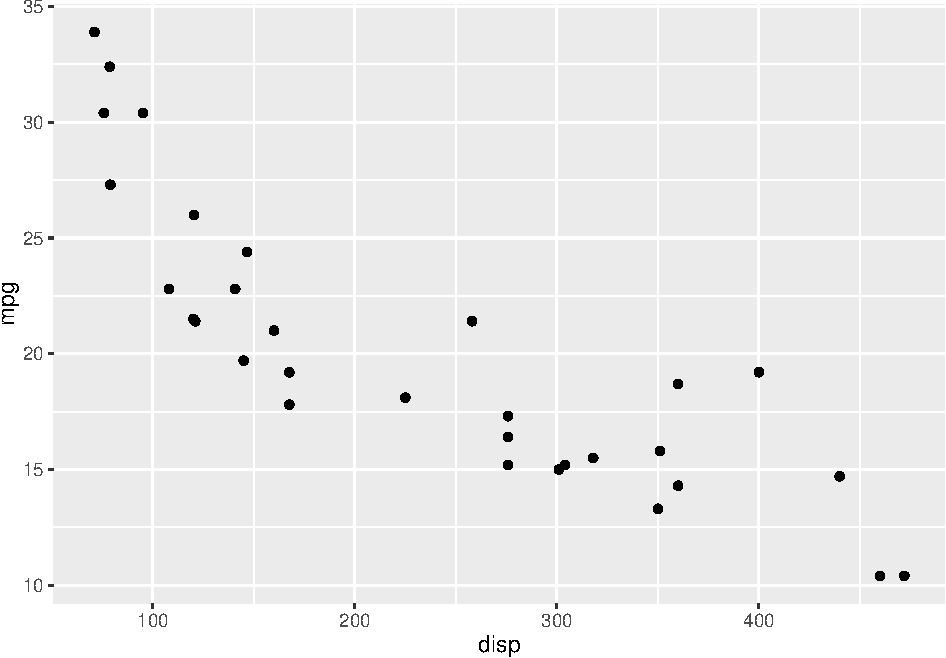
\includegraphics{curso-jurimetria_files/figure-latex/aula05chunk03-1.pdf}

Observe que o primeiro argumento da função \texttt{ggplot} é um data
frame. A função \texttt{aes()} descreve como as variáveis são mapeadas
em aspectos visuais de formas geométricas definidas pelos \emph{geoms}.
Aqui, essas formas geométricas são pontos, selecionados pela função
\texttt{geom\_point()}, gerando, assim, um gráfico de dispersão. A
combinação dessas duas camadas define o tipo de gráfico que você deseja
construir.

\subsubsection{Aesthetics}\label{aesthetics}

A primeira camada de um gráfico deve indicar a relação entre os dados e
cada aspecto visual do gráfico, como qual variável será representada no
eixo x, qual será representada no eixo y, a cor e o tamanho dos
componentes geométricos etc. Os aspectos que podem ou devem ser mapeados
depende do tipo de gráfico que você deseja fazer.

No exemplo acima, atribuímos aspectos de posição: ao eixo y mapeamos a
variável \texttt{mpg} (milhas por galão) e ao eixo x a variável
\texttt{disp} (cilindradas). Outro aspecto que pode ser mapeado nesse
gráfico é a cor dos pontos

\begin{Shaded}
\begin{Highlighting}[]
\KeywordTok{ggplot}\NormalTok{(}\DataTypeTok{data =} \NormalTok{mtcars, }\KeywordTok{aes}\NormalTok{(}\DataTypeTok{x =} \NormalTok{disp, }\DataTypeTok{y =} \NormalTok{mpg, }\DataTypeTok{colour =} \KeywordTok{as.factor}\NormalTok{(am))) +}\StringTok{ }
\StringTok{  }\KeywordTok{geom_point}\NormalTok{()}
\end{Highlighting}
\end{Shaded}

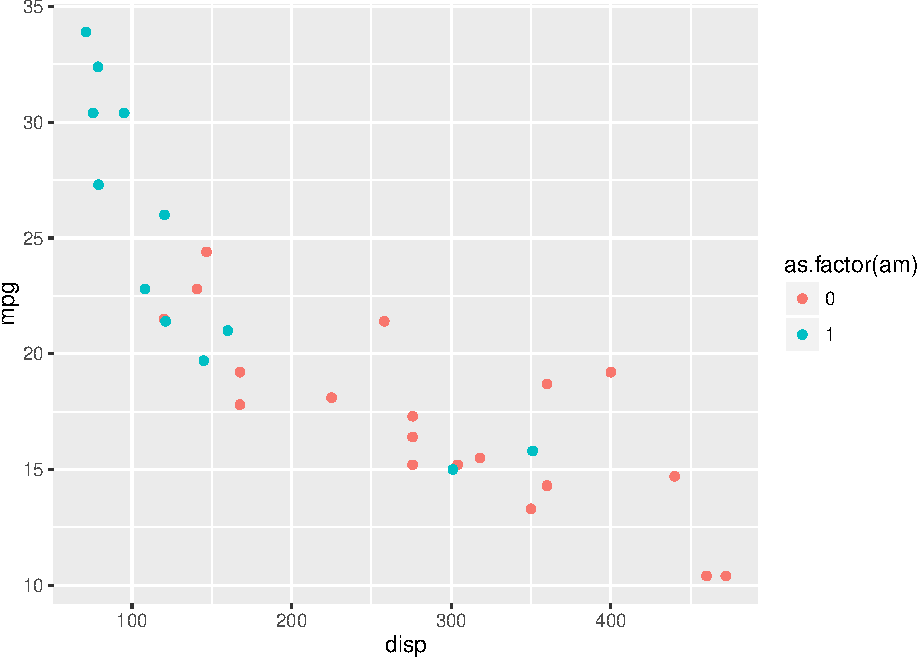
\includegraphics{curso-jurimetria_files/figure-latex/aula05chunk04-1.pdf}

Agora, a variável \texttt{am} (tipo de transmissão) foi mapeada à cor
dos pontos, sendo que pontos vermelhos correspondem à transmissão
automática (valor 0) e pontos azuis à transmissão manual (valor 1).
Observe que inserimos a variável \texttt{am} como um fator, pois temos
interesse apenas nos valores ``0'' e ``1''. No entanto, tambem podemos
mapear uma variável contínua à cor dos pontos:

\begin{Shaded}
\begin{Highlighting}[]
\KeywordTok{ggplot}\NormalTok{(mtcars, }\KeywordTok{aes}\NormalTok{(}\DataTypeTok{x =} \NormalTok{disp, }\DataTypeTok{y =} \NormalTok{mpg, }\DataTypeTok{colour =} \NormalTok{cyl)) +}\StringTok{ }
\StringTok{  }\KeywordTok{geom_point}\NormalTok{()}
\end{Highlighting}
\end{Shaded}

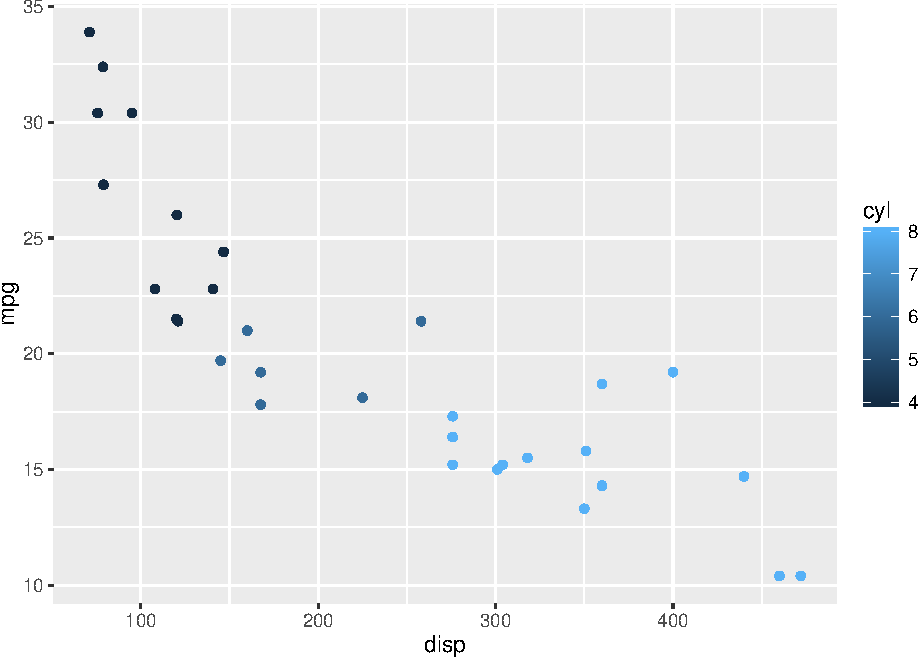
\includegraphics{curso-jurimetria_files/figure-latex/aula05chunk05-1.pdf}

Aqui, o número de cilindros, \texttt{cyl}, é representado pela
tonalidade da cor azul.

\textbf{Nota}: por \emph{default}, a legenda é insirida no gráfico
automaticamente.

Também podemos mapear o tamanho dos pontos à uma variável de interesse:

\begin{Shaded}
\begin{Highlighting}[]
\KeywordTok{ggplot}\NormalTok{(mtcars, }\KeywordTok{aes}\NormalTok{(}\DataTypeTok{x =} \NormalTok{disp, }\DataTypeTok{y =} \NormalTok{mpg, }\DataTypeTok{colour =} \NormalTok{cyl, }\DataTypeTok{size =} \NormalTok{wt)) +}
\StringTok{  }\KeywordTok{geom_point}\NormalTok{()}
\end{Highlighting}
\end{Shaded}

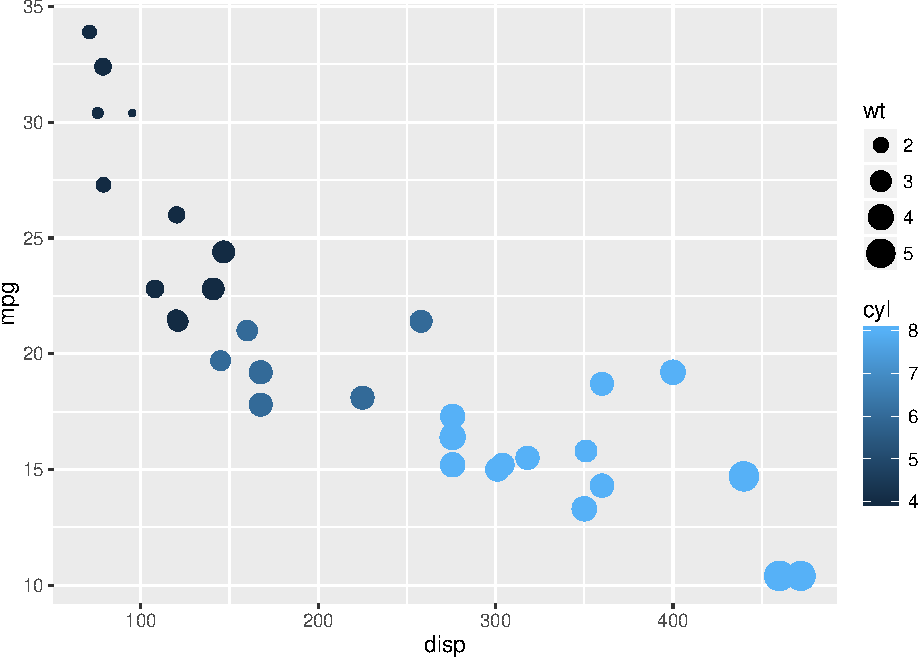
\includegraphics{curso-jurimetria_files/figure-latex/aula05chunk06-1.pdf}

\textbf{Exercício}: pesquisar mais aspectos que podem ser alterados no
gráfico de dispersão.

\subsubsection{Geoms}\label{geoms}

Os \emph{geoms} definem qual forma geométrica será utilizada para a
visualização dos dados no gráfico. Como já vimos, a função
\texttt{geom\_point()} gera gráficos de dispersão transformando pares
(x,y) em pontos. Veja a seguir outros \emph{geoms} bastante utilizados:

\begin{itemize}
\tightlist
\item
  geom\_line: para retas definidas por pares (x,y)
\item
  geom\_abline: para retas definidas por um intercepto e uma inclinação
\item
  geom\_hline: para retas horizontais
\item
  geom\_boxplot: para boxplots
\item
  geom\_histogram: para histogramas
\item
  geom\_density: para densidades
\item
  geom\_area: para áreas
\item
  geom\_bar: para barras
\end{itemize}

Veja a seguir como é fácil gerar diversos gráficos diferentes utilizando
a mesma estrutura do gráfico de dispersão acima:

\begin{Shaded}
\begin{Highlighting}[]
\KeywordTok{ggplot}\NormalTok{(mtcars, }\KeywordTok{aes}\NormalTok{(}\DataTypeTok{x =} \KeywordTok{as.factor}\NormalTok{(cyl), }\DataTypeTok{y =} \NormalTok{mpg)) +}\StringTok{ }
\StringTok{  }\KeywordTok{geom_boxplot}\NormalTok{()}
\end{Highlighting}
\end{Shaded}

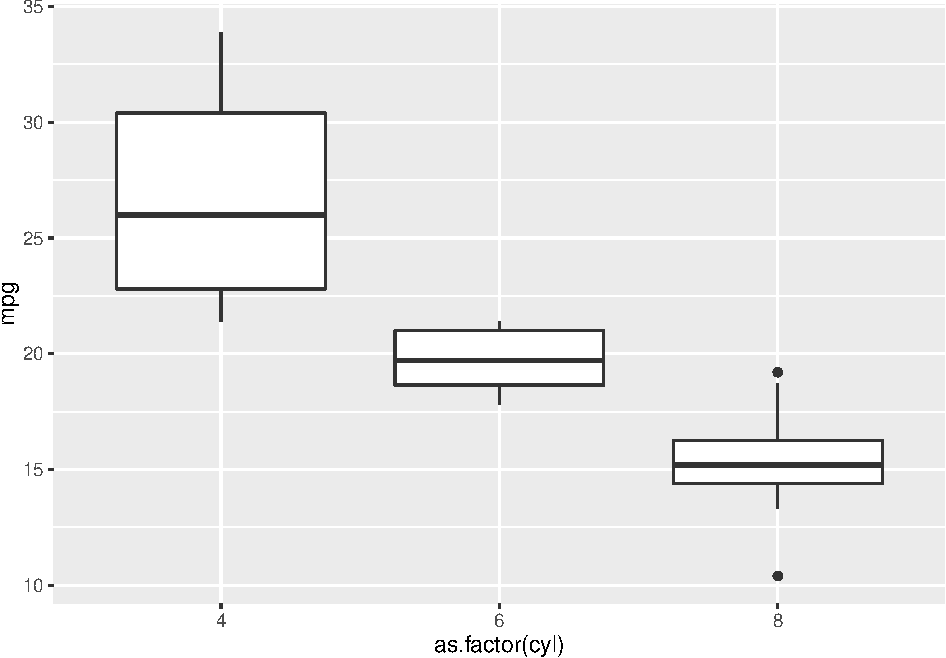
\includegraphics{curso-jurimetria_files/figure-latex/aula05chunk07-1.pdf}

\begin{Shaded}
\begin{Highlighting}[]
\KeywordTok{ggplot}\NormalTok{(mtcars, }\KeywordTok{aes}\NormalTok{(}\DataTypeTok{x =} \NormalTok{mpg)) +}\StringTok{ }
\StringTok{  }\KeywordTok{geom_histogram}\NormalTok{()}
\end{Highlighting}
\end{Shaded}

\begin{verbatim}
## `stat_bin()` using `bins = 30`. Pick better value with `binwidth`.
\end{verbatim}

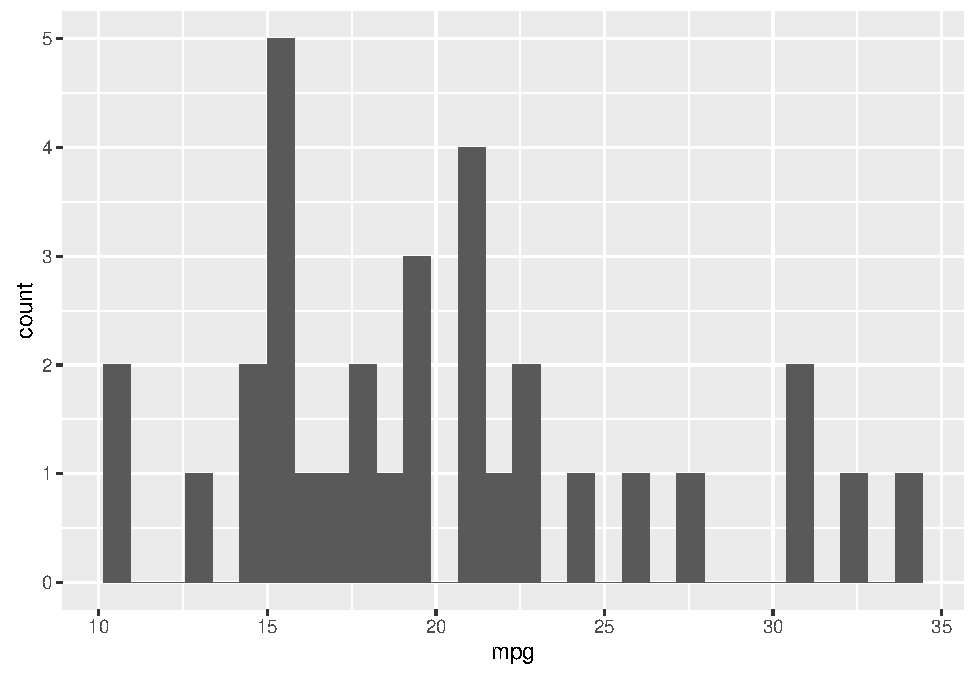
\includegraphics{curso-jurimetria_files/figure-latex/aula05chunk08-1.pdf}

\begin{Shaded}
\begin{Highlighting}[]
\KeywordTok{ggplot}\NormalTok{(mtcars, }\KeywordTok{aes}\NormalTok{(}\DataTypeTok{x =} \KeywordTok{as.factor}\NormalTok{(cyl))) +}\StringTok{ }
\StringTok{  }\KeywordTok{geom_bar}\NormalTok{()}
\end{Highlighting}
\end{Shaded}

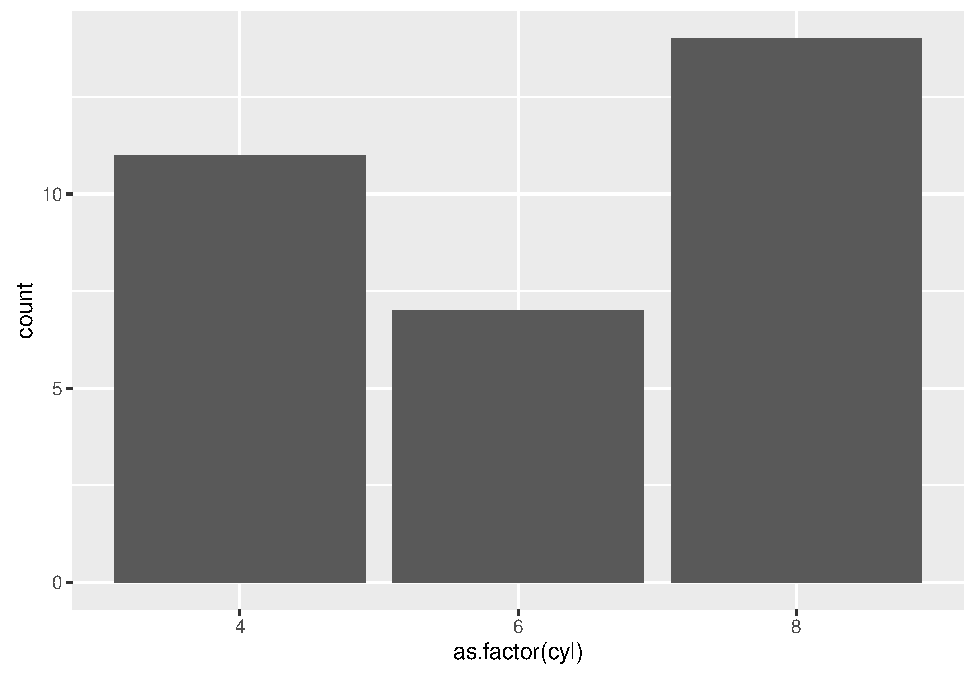
\includegraphics{curso-jurimetria_files/figure-latex/aula05chunk09-1.pdf}

Para fazer um boxplot para cada grupo, precisamos passar para o aspecto
x do gráfico uma variável do tipo fator. \#\#\# Personalizando os
gráficos

\subsubsection{Cores}\label{cores}

O aspecto colour do boxplot, muda a cor do contorno. Para mudar o
preenchimento, basta usar o \texttt{fill}.

\begin{Shaded}
\begin{Highlighting}[]
\KeywordTok{ggplot}\NormalTok{(mtcars, }\KeywordTok{aes}\NormalTok{(}\DataTypeTok{x =} \KeywordTok{as.factor}\NormalTok{(cyl), }\DataTypeTok{y =} \NormalTok{mpg, }\DataTypeTok{colour =} \KeywordTok{as.factor}\NormalTok{(cyl))) +}\StringTok{ }
\StringTok{  }\KeywordTok{geom_boxplot}\NormalTok{()}
\end{Highlighting}
\end{Shaded}

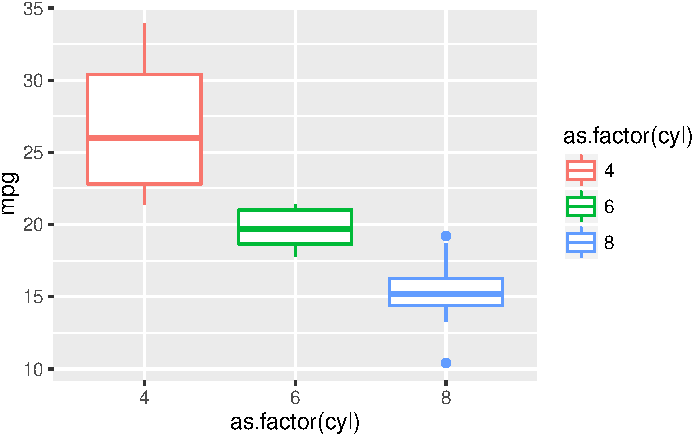
\includegraphics{curso-jurimetria_files/figure-latex/aula05chunk10-1.pdf}

\begin{Shaded}
\begin{Highlighting}[]
\KeywordTok{ggplot}\NormalTok{(mtcars, }\KeywordTok{aes}\NormalTok{(}\DataTypeTok{x =} \KeywordTok{as.factor}\NormalTok{(cyl), }\DataTypeTok{y =} \NormalTok{mpg, }\DataTypeTok{fill =} \KeywordTok{as.factor}\NormalTok{(cyl))) +}\StringTok{ }\KeywordTok{geom_boxplot}\NormalTok{()}
\end{Highlighting}
\end{Shaded}

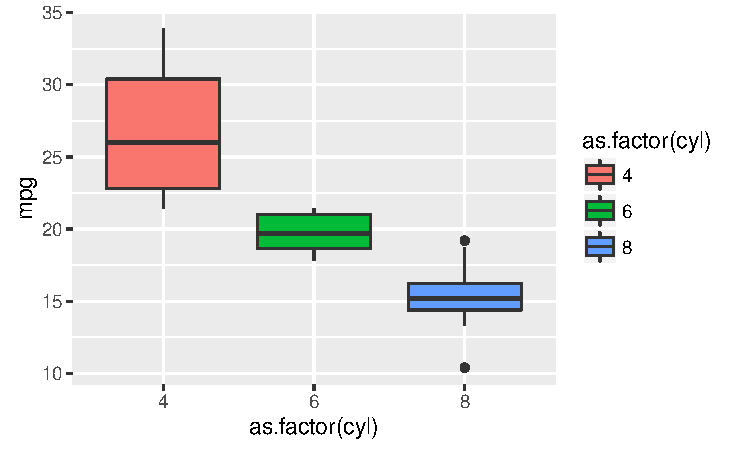
\includegraphics{curso-jurimetria_files/figure-latex/aula05chunk11-1.pdf}

Você pode também mudar a cor dos objetos sem mapeá-la a uma variável.
Para isso, observe que os aspectos \texttt{colour} e \texttt{fill} são
especificados fora do \texttt{aes()}.

\begin{Shaded}
\begin{Highlighting}[]
\KeywordTok{ggplot}\NormalTok{(mtcars, }\KeywordTok{aes}\NormalTok{(}\DataTypeTok{x =} \KeywordTok{as.factor}\NormalTok{(cyl), }\DataTypeTok{y =} \NormalTok{mpg)) +}\StringTok{ }
\StringTok{  }\KeywordTok{geom_boxplot}\NormalTok{(}\DataTypeTok{color =} \StringTok{"red"}\NormalTok{, }\DataTypeTok{fill =} \StringTok{"pink"}\NormalTok{)}
\end{Highlighting}
\end{Shaded}

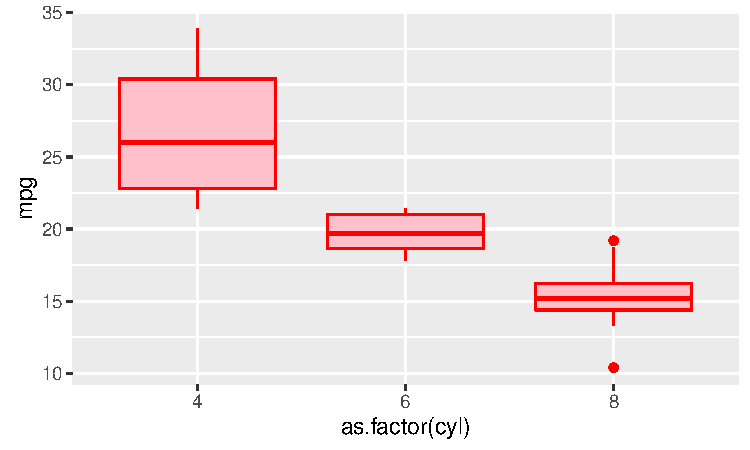
\includegraphics{curso-jurimetria_files/figure-latex/aula05chunk12-1.pdf}

\subsubsection{Eixos}\label{eixos}

Para alterar os labels dos eixos acrescentamos as funções
\texttt{xlab()} ou \texttt{ylab()}.

\begin{Shaded}
\begin{Highlighting}[]
\KeywordTok{ggplot}\NormalTok{(mtcars, }\KeywordTok{aes}\NormalTok{(}\DataTypeTok{x =} \NormalTok{mpg)) +}\StringTok{ }
\StringTok{  }\KeywordTok{geom_histogram}\NormalTok{() +}
\StringTok{  }\KeywordTok{xlab}\NormalTok{(}\StringTok{"Milhas por galão"}\NormalTok{) +}
\StringTok{  }\KeywordTok{ylab}\NormalTok{(}\StringTok{"Frequência"}\NormalTok{)}
\end{Highlighting}
\end{Shaded}

\begin{verbatim}
## `stat_bin()` using `bins = 30`. Pick better value with `binwidth`.
\end{verbatim}

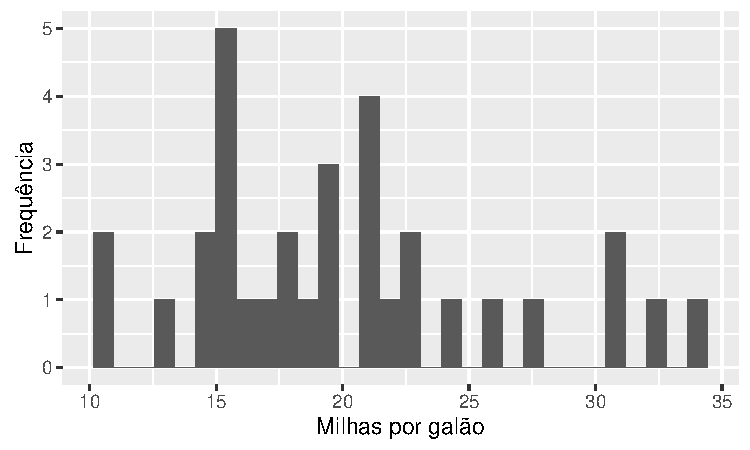
\includegraphics{curso-jurimetria_files/figure-latex/aula05chunk13-1.pdf}

Para alterar os limites dos gráficos usamos as funções \texttt{xlim()} e
\texttt{ylim()}.

\begin{Shaded}
\begin{Highlighting}[]
\KeywordTok{ggplot}\NormalTok{(mtcars, }\KeywordTok{aes}\NormalTok{(}\DataTypeTok{x =} \NormalTok{mpg)) +}\StringTok{ }
\StringTok{  }\KeywordTok{geom_histogram}\NormalTok{() +}
\StringTok{  }\KeywordTok{xlab}\NormalTok{(}\StringTok{"Milhas por galão"}\NormalTok{) +}
\StringTok{  }\KeywordTok{ylab}\NormalTok{(}\StringTok{"Frequência"}\NormalTok{) +}
\StringTok{  }\KeywordTok{xlim}\NormalTok{(}\KeywordTok{c}\NormalTok{(}\DecValTok{0}\NormalTok{, }\DecValTok{40}\NormalTok{)) +}
\StringTok{  }\KeywordTok{ylim}\NormalTok{(}\KeywordTok{c}\NormalTok{(}\DecValTok{0}\NormalTok{,}\DecValTok{8}\NormalTok{))}
\end{Highlighting}
\end{Shaded}

\begin{verbatim}
## `stat_bin()` using `bins = 30`. Pick better value with `binwidth`.
\end{verbatim}

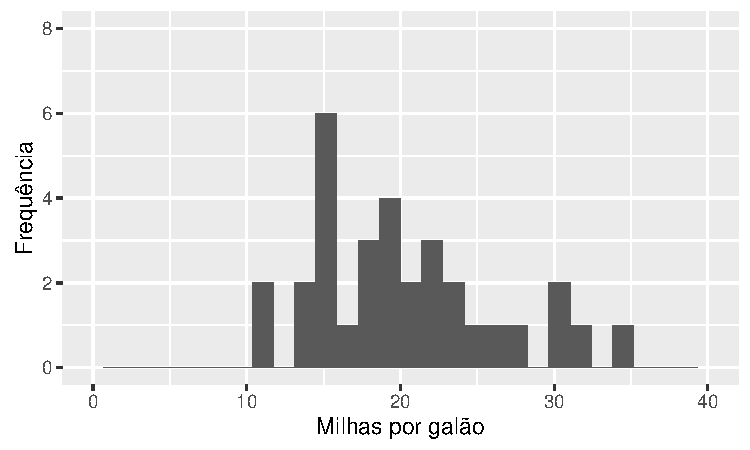
\includegraphics{curso-jurimetria_files/figure-latex/aula05chunk14-1.pdf}

\subsubsection{Legendas}\label{legendas}

A legenda de um gráfico pode ser facilmente personalizada.

Para trocar o \emph{label} da leganda:

\begin{Shaded}
\begin{Highlighting}[]
\KeywordTok{ggplot}\NormalTok{(mtcars, }\KeywordTok{aes}\NormalTok{(}\DataTypeTok{x =} \KeywordTok{as.factor}\NormalTok{(cyl), }\DataTypeTok{fill =} \KeywordTok{as.factor}\NormalTok{(cyl))) +}\StringTok{ }
\StringTok{  }\KeywordTok{geom_bar}\NormalTok{() +}
\StringTok{  }\KeywordTok{labs}\NormalTok{(}\DataTypeTok{fill =} \StringTok{"cyl"}\NormalTok{)}
\end{Highlighting}
\end{Shaded}

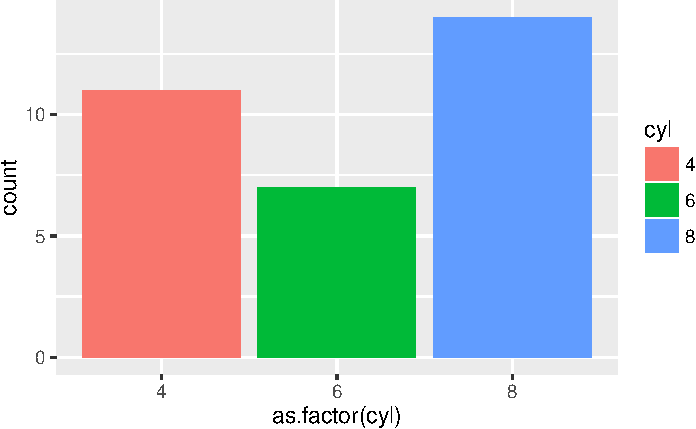
\includegraphics{curso-jurimetria_files/figure-latex/aula05chunk15-1.pdf}

Para trocar a posição da legenda:

\begin{Shaded}
\begin{Highlighting}[]
\KeywordTok{ggplot}\NormalTok{(mtcars, }\KeywordTok{aes}\NormalTok{(}\DataTypeTok{x =} \KeywordTok{as.factor}\NormalTok{(cyl), }\DataTypeTok{fill =} \KeywordTok{as.factor}\NormalTok{(cyl))) +}\StringTok{ }
\StringTok{  }\KeywordTok{geom_bar}\NormalTok{() +}
\StringTok{  }\KeywordTok{labs}\NormalTok{(}\DataTypeTok{fill =} \StringTok{"cyl"}\NormalTok{) +}
\StringTok{  }\KeywordTok{theme}\NormalTok{(}\DataTypeTok{legend.position=}\StringTok{"top"}\NormalTok{)}
\end{Highlighting}
\end{Shaded}

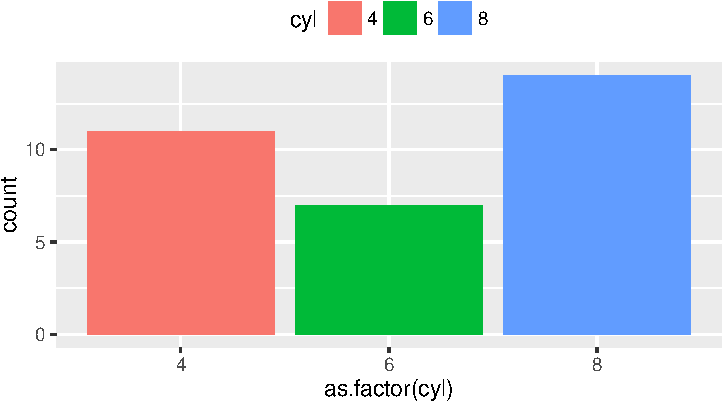
\includegraphics{curso-jurimetria_files/figure-latex/aula05chunk16-1.pdf}

Para retirar a legenda:

\begin{Shaded}
\begin{Highlighting}[]
\KeywordTok{ggplot}\NormalTok{(mtcars, }\KeywordTok{aes}\NormalTok{(}\DataTypeTok{x =} \KeywordTok{as.factor}\NormalTok{(cyl), }\DataTypeTok{fill =} \KeywordTok{as.factor}\NormalTok{(cyl))) +}\StringTok{ }
\StringTok{  }\KeywordTok{geom_bar}\NormalTok{() +}
\StringTok{  }\KeywordTok{guides}\NormalTok{(}\DataTypeTok{fill=}\OtherTok{FALSE}\NormalTok{)}
\end{Highlighting}
\end{Shaded}

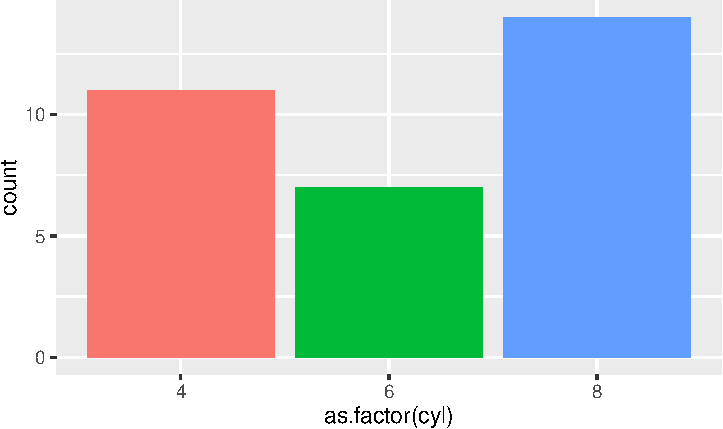
\includegraphics{curso-jurimetria_files/figure-latex/aula05chunk17-1.pdf}

Veja mais opções de personalização
\href{http://www.cookbook-r.com/Graphs/Legends_(ggplot2)/}{aqui!}

\subsubsection{Facets}\label{facets}

Outra funcionalidade muito importante do ggplot é o uso de
\emph{facets}.

\begin{Shaded}
\begin{Highlighting}[]
\KeywordTok{ggplot}\NormalTok{(mtcars, }\KeywordTok{aes}\NormalTok{(}\DataTypeTok{x =} \NormalTok{mpg, }\DataTypeTok{y =} \NormalTok{disp, }\DataTypeTok{colour =} \KeywordTok{as.factor}\NormalTok{(cyl))) +}\StringTok{ }
\StringTok{  }\KeywordTok{geom_point}\NormalTok{() +}\StringTok{ }
\StringTok{  }\KeywordTok{facet_grid}\NormalTok{(am~.)}
\end{Highlighting}
\end{Shaded}

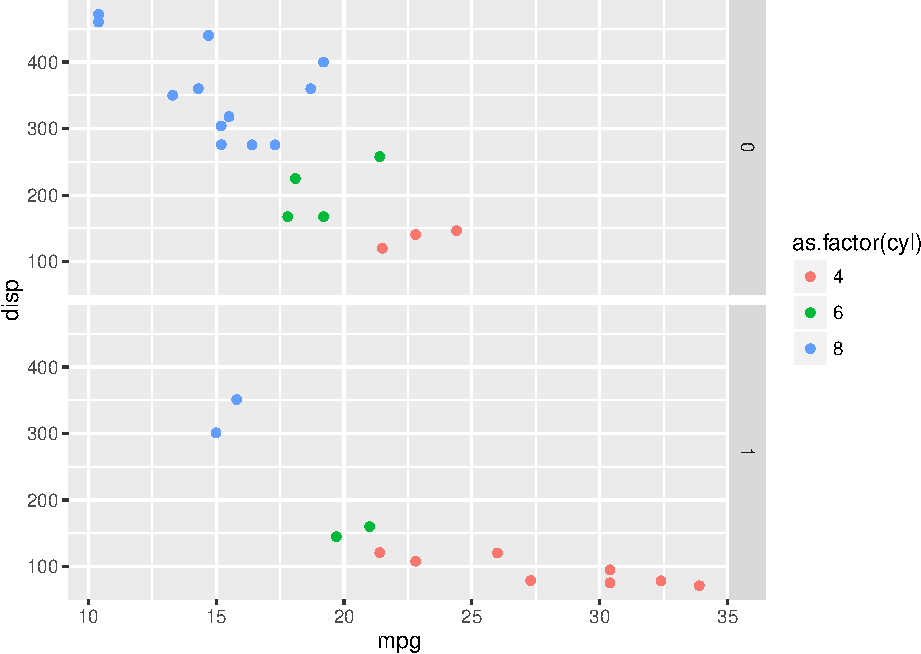
\includegraphics{curso-jurimetria_files/figure-latex/aula05chunk18-1.pdf}

Podemos colocar os graficos lado a lado também:

\begin{Shaded}
\begin{Highlighting}[]
\KeywordTok{ggplot}\NormalTok{(mtcars, }\KeywordTok{aes}\NormalTok{(}\DataTypeTok{x =} \NormalTok{mpg, }\DataTypeTok{y =} \NormalTok{disp, }\DataTypeTok{colour =} \KeywordTok{as.factor}\NormalTok{(cyl))) +}
\StringTok{  }\KeywordTok{geom_point}\NormalTok{() +}\StringTok{ }
\StringTok{  }\KeywordTok{facet_grid}\NormalTok{(.~am)}
\end{Highlighting}
\end{Shaded}

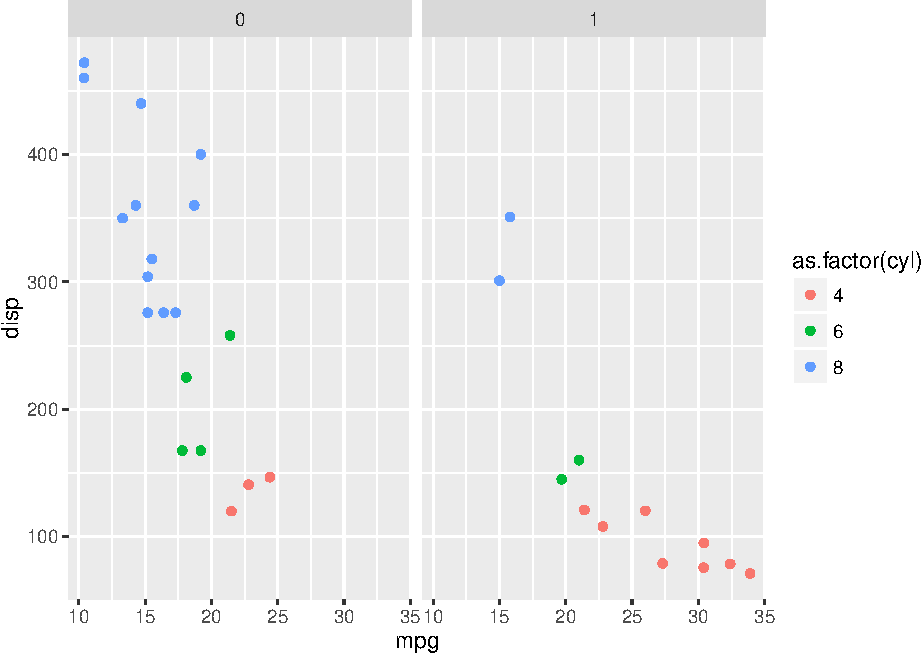
\includegraphics{curso-jurimetria_files/figure-latex/aula05chunk19-1.pdf}

\section{Exemplo visualização}\label{exemplo-visualizacao}

No exemplo das câmaras, vamos fazer três gráficos. O primeiro mostra a
proporção de processos por assunto em cada câmara.

\begin{Shaded}
\begin{Highlighting}[]
\NormalTok{d_cjsg %>%}
\StringTok{  }\KeywordTok{separate}\NormalTok{(classe_assunto, }\KeywordTok{c}\NormalTok{(}\StringTok{'classe'}\NormalTok{, }\StringTok{'assunto'}\NormalTok{), }\DataTypeTok{sep =} \StringTok{' / '}\NormalTok{, }
           \DataTypeTok{extra =} \StringTok{'merge'}\NormalTok{, }\DataTypeTok{fill =} \StringTok{'right'}\NormalTok{) %>%}\StringTok{ }
\StringTok{  }\KeywordTok{group_by}\NormalTok{(assunto) %>%}\StringTok{ }
\StringTok{  }\KeywordTok{mutate}\NormalTok{(}\DataTypeTok{n_assunto =} \KeywordTok{n}\NormalTok{()) %>%}\StringTok{ }
\StringTok{  }\KeywordTok{ungroup}\NormalTok{() %>%}\StringTok{ }
\StringTok{  }\KeywordTok{mutate}\NormalTok{(}\DataTypeTok{assunto =} \KeywordTok{ifelse}\NormalTok{(n_assunto <}\StringTok{ }\DecValTok{5000}\NormalTok{, }\StringTok{'Outro'}\NormalTok{, assunto)) %>%}\StringTok{ }
\StringTok{  }\KeywordTok{count}\NormalTok{(orgao_julgador, assunto) %>%}
\StringTok{  }\KeywordTok{mutate}\NormalTok{(}\DataTypeTok{ntot =} \KeywordTok{sum}\NormalTok{(n), }\DataTypeTok{prop =} \NormalTok{n /}\StringTok{ }\NormalTok{ntot) %>%}
\StringTok{  }\NormalTok{ungroup %>%}
\StringTok{  }\KeywordTok{filter}\NormalTok{(ntot >}\StringTok{ }\DecValTok{1000}\NormalTok{) %>%}\StringTok{ }
\StringTok{  }\KeywordTok{mutate}\NormalTok{(}\DataTypeTok{num =} \KeywordTok{extract_numeric}\NormalTok{(orgao_julgador),}
         \DataTypeTok{num =} \KeywordTok{sprintf}\NormalTok{(}\StringTok{'%02d'}\NormalTok{, num)) %>%}\StringTok{ }
\StringTok{  }\KeywordTok{mutate}\NormalTok{(}\DataTypeTok{extra =} \KeywordTok{str_detect}\NormalTok{(orgao_julgador, }\StringTok{'Extra'}\NormalTok{),}
         \DataTypeTok{extra =} \KeywordTok{ifelse}\NormalTok{(extra, }\StringTok{'Câmara Extraordinária'}\NormalTok{, }
                        \StringTok{'Câmara de Direito Criminal'}\NormalTok{)) %>%}\StringTok{ }
\StringTok{  }\KeywordTok{ggplot}\NormalTok{(}\KeywordTok{aes}\NormalTok{(}\DataTypeTok{x =} \NormalTok{num, }\DataTypeTok{fill =} \NormalTok{assunto, }\DataTypeTok{y =} \NormalTok{prop)) +}
\StringTok{  }\KeywordTok{geom_bar}\NormalTok{(}\DataTypeTok{stat =} \StringTok{'identity'}\NormalTok{, }\DataTypeTok{colour =} \StringTok{'black'}\NormalTok{) +}
\StringTok{  }\KeywordTok{facet_wrap}\NormalTok{(~extra, }\DataTypeTok{scales =} \StringTok{'free_x'}\NormalTok{) +}
\StringTok{  }\KeywordTok{theme_bw}\NormalTok{() +}
\StringTok{  }\KeywordTok{scale_y_continuous}\NormalTok{(}\DataTypeTok{labels =} \NormalTok{scales::percent) +}
\StringTok{  }\KeywordTok{xlab}\NormalTok{(}\StringTok{'Órgão julgador'}\NormalTok{) +}
\StringTok{  }\KeywordTok{ylab}\NormalTok{(}\StringTok{'Proporção de processos por assunto'}\NormalTok{) +}
\StringTok{  }\KeywordTok{theme}\NormalTok{(}\DataTypeTok{legend.position =} \StringTok{"bottom"}\NormalTok{)}
\end{Highlighting}
\end{Shaded}

\begin{verbatim}
## extract_numeric() is deprecated: please use readr::parse_numeric() instead
\end{verbatim}

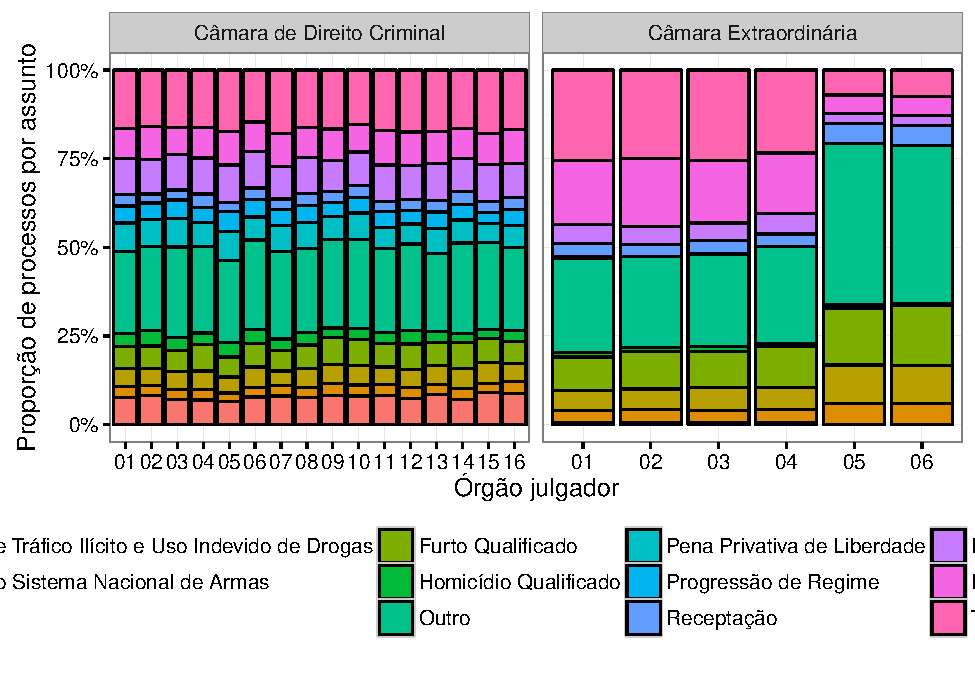
\includegraphics{curso-jurimetria_files/figure-latex/unnamed-chunk-61-1.pdf}

O segundo mostra a proporção de decisões favoráveis no tempo.

\begin{Shaded}
\begin{Highlighting}[]
\NormalTok{partes_apelacoes <-}\StringTok{ }\NormalTok{d_partes %>%}\StringTok{ }
\StringTok{  }\KeywordTok{filter}\NormalTok{(tipo ==}\StringTok{ 'apelado'}\NormalTok{, }\KeywordTok{str_detect}\NormalTok{(nome, }\StringTok{'[Mm]inist'}\NormalTok{)) %>%}\StringTok{ }
\StringTok{  }\KeywordTok{mutate}\NormalTok{(}\DataTypeTok{n_processo =} \KeywordTok{str_replace_all}\NormalTok{(arq, }\StringTok{'[^0-9]'}\NormalTok{, }\StringTok{''}\NormalTok{)) %>%}\StringTok{ }
\StringTok{  }\KeywordTok{select}\NormalTok{(n_processo)}
  
\NormalTok{decisoes <-}\StringTok{ }\NormalTok{d_decisoes %>%}\StringTok{ }
\StringTok{  }\KeywordTok{mutate}\NormalTok{(}\DataTypeTok{n_processo =} \KeywordTok{str_replace_all}\NormalTok{(arq, }\StringTok{'[^0-9]'}\NormalTok{, }\StringTok{''}\NormalTok{)) %>%}\StringTok{ }
\StringTok{  }\KeywordTok{inner_join}\NormalTok{(partes_apelacoes, }\StringTok{'n_processo'}\NormalTok{) %>%}\StringTok{ }
\StringTok{  }\KeywordTok{filter}\NormalTok{(situacao ==}\StringTok{ 'Julgado'}\NormalTok{) %>%}\StringTok{ }
\StringTok{  }\KeywordTok{distinct}\NormalTok{(n_processo, decisao) %>%}
\StringTok{  }\KeywordTok{mutate}\NormalTok{(}\DataTypeTok{tipo_decisao =} \KeywordTok{tipos_decisao}\NormalTok{(decisao)) %>%}\StringTok{ }
\StringTok{  }\KeywordTok{select}\NormalTok{(n_processo, tipo_decisao)}
  

\NormalTok{aux <-}\StringTok{ }\NormalTok{d_cjsg %>%}
\StringTok{  }\KeywordTok{mutate}\NormalTok{(}\DataTypeTok{n_processo =} \KeywordTok{str_replace_all}\NormalTok{(n_processo, }\StringTok{'[^0-9]'}\NormalTok{, }\StringTok{''}\NormalTok{)) %>%}\StringTok{ }
\StringTok{  }\KeywordTok{inner_join}\NormalTok{(decisoes, }\StringTok{'n_processo'}\NormalTok{) %>%}\StringTok{ }
\StringTok{  }\KeywordTok{arrange}\NormalTok{(}\KeywordTok{desc}\NormalTok{(}\KeywordTok{dmy}\NormalTok{(data_julgamento))) %>%}\StringTok{ }
\StringTok{  }\KeywordTok{distinct}\NormalTok{(n_processo, }\DataTypeTok{.keep_all =} \OtherTok{TRUE}\NormalTok{) %>%}\StringTok{ }
\StringTok{  }\KeywordTok{mutate}\NormalTok{(}\DataTypeTok{data =} \KeywordTok{dmy}\NormalTok{(data_julgamento)) %>%}
\StringTok{  }\KeywordTok{mutate}\NormalTok{(}\DataTypeTok{ano_mes =} \KeywordTok{floor_date}\NormalTok{(data, }\StringTok{'month'}\NormalTok{))}

\NormalTok{aux %>%}
\StringTok{  }\KeywordTok{count}\NormalTok{(ano_mes, tipo_decisao) %>%}
\StringTok{  }\KeywordTok{mutate}\NormalTok{(}\DataTypeTok{prop =} \NormalTok{n/}\KeywordTok{sum}\NormalTok{(n)) %>%}
\StringTok{  }\NormalTok{ungroup %>%}
\StringTok{  }\KeywordTok{ggplot}\NormalTok{(}\KeywordTok{aes}\NormalTok{(}\DataTypeTok{x =} \NormalTok{ano_mes, }\DataTypeTok{y =} \NormalTok{prop, }\DataTypeTok{colour =} \NormalTok{tipo_decisao)) +}
\StringTok{  }\KeywordTok{geom_line}\NormalTok{() +}
\StringTok{  }\KeywordTok{geom_text}\NormalTok{(}\KeywordTok{aes}\NormalTok{(}\DataTypeTok{y =} \FloatTok{0.65}\NormalTok{, }\DataTypeTok{label =} \NormalTok{n, }\DataTypeTok{colour =} \OtherTok{NULL}\NormalTok{), }
            \DataTypeTok{data =} \KeywordTok{count}\NormalTok{(aux, ano_mes)) +}
\StringTok{  }\KeywordTok{scale_x_date}\NormalTok{(}\DataTypeTok{breaks =} \NormalTok{scales::}\KeywordTok{date_breaks}\NormalTok{(}\StringTok{'1 month'}\NormalTok{),}
               \DataTypeTok{labels =} \NormalTok{scales::}\KeywordTok{date_format}\NormalTok{(}\StringTok{"%b"}\NormalTok{)) +}
\StringTok{  }\KeywordTok{scale_y_continuous}\NormalTok{(}\DataTypeTok{labels =} \NormalTok{scales::percent) +}
\StringTok{  }\KeywordTok{xlab}\NormalTok{(}\StringTok{'Tempo (meses)'}\NormalTok{) +}
\StringTok{  }\KeywordTok{ylab}\NormalTok{(}\StringTok{'Proporção de cada tipo de decisão'}\NormalTok{) +}
\StringTok{  }\KeywordTok{theme_bw}\NormalTok{()}
\end{Highlighting}
\end{Shaded}

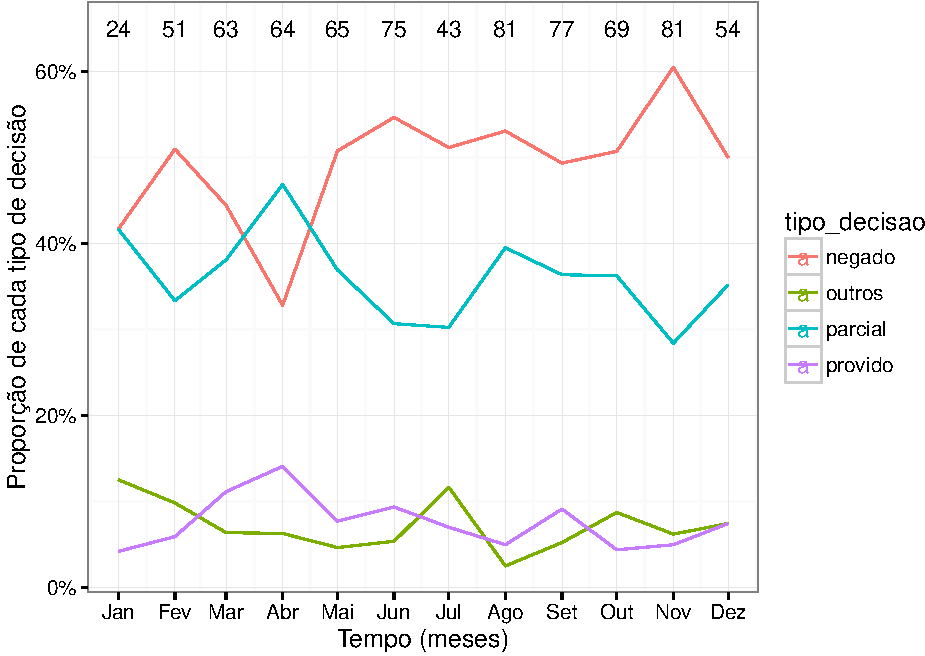
\includegraphics{curso-jurimetria_files/figure-latex/unnamed-chunk-62-1.pdf}

O terceiro mostra a proporção de cada tipo de decisão em cada câmara.

\begin{Shaded}
\begin{Highlighting}[]
\NormalTok{d_cjsg %>%}
\StringTok{  }\KeywordTok{mutate}\NormalTok{(}\DataTypeTok{n_processo =} \KeywordTok{str_replace_all}\NormalTok{(n_processo, }\StringTok{'[^0-9]'}\NormalTok{, }\StringTok{''}\NormalTok{)) %>%}\StringTok{ }
\StringTok{  }\KeywordTok{inner_join}\NormalTok{(decisoes, }\StringTok{'n_processo'}\NormalTok{) %>%}\StringTok{ }
\StringTok{  }\KeywordTok{count}\NormalTok{(orgao_julgador, tipo_decisao) %>%}
\StringTok{  }\KeywordTok{mutate}\NormalTok{(}\DataTypeTok{ntot =} \KeywordTok{sum}\NormalTok{(n), }\DataTypeTok{prop =} \NormalTok{n /}\StringTok{ }\NormalTok{ntot) %>%}
\StringTok{  }\KeywordTok{ungroup}\NormalTok{() %>%}
\StringTok{  }\KeywordTok{filter}\NormalTok{(ntot >}\StringTok{ }\DecValTok{10}\NormalTok{) %>%}\StringTok{ }
\StringTok{  }\KeywordTok{mutate}\NormalTok{(}\DataTypeTok{num =} \KeywordTok{extract_numeric}\NormalTok{(orgao_julgador),}
         \DataTypeTok{num =} \KeywordTok{sprintf}\NormalTok{(}\StringTok{'%02d'}\NormalTok{, num)) %>%}\StringTok{ }
\StringTok{  }\KeywordTok{mutate}\NormalTok{(}\DataTypeTok{extra =} \KeywordTok{str_detect}\NormalTok{(orgao_julgador, }\StringTok{'Extra'}\NormalTok{),}
         \DataTypeTok{extra =} \KeywordTok{ifelse}\NormalTok{(extra, }\StringTok{'Câmara Extraordinária'}\NormalTok{, }
                        \StringTok{'Câmara de Direito Criminal'}\NormalTok{)) %>%}\StringTok{ }
\StringTok{  }\KeywordTok{ggplot}\NormalTok{(}\KeywordTok{aes}\NormalTok{(}\DataTypeTok{x =} \NormalTok{num, }\DataTypeTok{fill =} \NormalTok{tipo_decisao, }\DataTypeTok{y =} \NormalTok{prop)) +}
\StringTok{  }\KeywordTok{geom_bar}\NormalTok{(}\DataTypeTok{stat =} \StringTok{'identity'}\NormalTok{, }\DataTypeTok{colour =} \StringTok{'black'}\NormalTok{, }\DataTypeTok{position =} \StringTok{'dodge'}\NormalTok{) +}
\StringTok{  }\KeywordTok{facet_wrap}\NormalTok{(~extra, }\DataTypeTok{scales =} \StringTok{'free_x'}\NormalTok{) +}
\StringTok{  }\KeywordTok{theme_bw}\NormalTok{() +}
\StringTok{  }\KeywordTok{scale_y_continuous}\NormalTok{(}\DataTypeTok{labels =} \NormalTok{scales::percent) +}
\StringTok{  }\KeywordTok{xlab}\NormalTok{(}\StringTok{'Órgão julgador'}\NormalTok{) +}
\StringTok{  }\KeywordTok{ylab}\NormalTok{(}\StringTok{'Proporção de processos por tipo de decisão'}\NormalTok{) +}
\StringTok{  }\KeywordTok{theme}\NormalTok{(}\DataTypeTok{legend.position =} \StringTok{"bottom"}\NormalTok{)}
\end{Highlighting}
\end{Shaded}

\begin{verbatim}
## extract_numeric() is deprecated: please use readr::parse_numeric() instead
\end{verbatim}

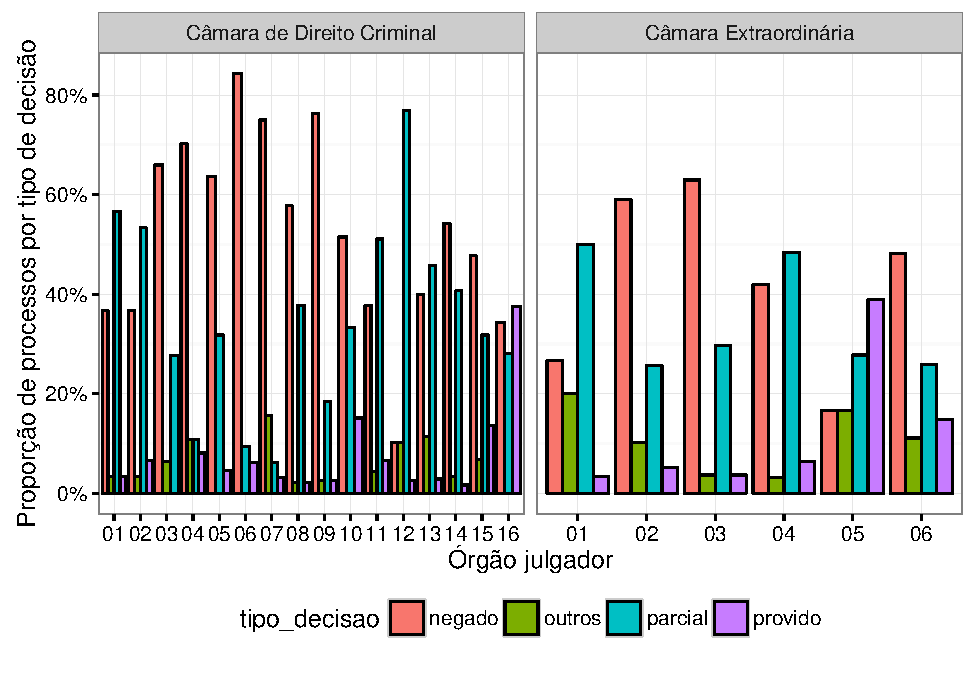
\includegraphics{curso-jurimetria_files/figure-latex/unnamed-chunk-63-1.pdf}

\section{\texorpdfstring{Ferramentas de visualização com
\texttt{shiny}}{Ferramentas de visualização com shiny}}\label{ferramentas-de-visualizacao-com-shiny}

O Shiny é um sistema para desenvolvimento de aplicações web usando o R,
um pacote do R (\texttt{shiny}) e um servidor web
(\texttt{shiny\ server}). O Shiny não é uma página web não é um
substituto para sistemas mais gerais, como Ruby on Rails e Django e não
é uma ferramenta gerencial, como o Tableau.

Para entender sobre Shiny, é necessário entender primeiro o que é
\href{http://programmers.stackexchange.com/a/171210}{server side e user
side}. Quando surfamos na web, nos \emph{comunicamos} com servidores do
mundo inteiro, geralmente através do protocolo HTTP.

No server side, processamos requisições e dados do cliente, estrutura e
envia páginas web, interage com banco de dados, etc. Linguagens server
side comuns são PHP, C\#, Java, R etc (virtualmente qualquer linguagem
de programação).

No user side, criamos interfaces gráficas a partir dos códigos recebidos
pelo servidor, envia e recebe informações do servidor etc. As
``linguagens'' mais usuais nesse caso são HTML, CSS e JavaScript.

Mas onde está o Shiny nisso tudo? O código de uma aplicação shiny fica
no \emph{server side}. O shiny permite que um computador (servidor)
envie páginas web, receba informações do usuário e processe dados,
utilizando apenas o R. Para rodar aplicativos shiny, geralmente
estruturamos a parte relacionada ao HTML, JavaScript e CSS no arquivo
\texttt{ui.R}, e a parte relacionada com processamento de dados e
geração de gráficos e análises no arquivo \texttt{server.R}. Os arquivos
\texttt{ui.R} e \texttt{server.R} ficam no servidor! Atualmente é
possível construir
\href{http://shiny.rstudio.com/articles/single-file.html}{aplicativos em
um arquivo só}, mas vamos manter a estrutura de \texttt{ui.R} e
\texttt{server.R}.

O pacote \texttt{shiny} do R possui internamente um servidor web básico,
geralmente utilizado para aplicações locais, permitindo somente uma
aplicação por vez. O \texttt{shiny\ server} é um programa que roda
somente em Linux que permite o acesso a múltiplas aplicações
simultaneamente.

\subsection{Começando com um exemplo}\label{comecando-com-um-exemplo}

\begin{Shaded}
\begin{Highlighting}[]
\NormalTok{shiny::}\KeywordTok{runGitHub}\NormalTok{(}\StringTok{'abjur/vistemplate'}\NormalTok{, }\DataTypeTok{subdir=}\StringTok{'exemplo_01_helloworld'}\NormalTok{)}
\end{Highlighting}
\end{Shaded}

O Shiny utiliza como padrão o
\href{http://getbootstrap.com/css/}{bootstrap css} do
\href{https://twitter.com}{Twitter}, que é bonito e responsivo (lida bem
com várias plataformas, como notebook e mobile). Note que criamos
páginas básicas com \texttt{pageWithSidebar}. Páginas mais trabalhadas
são criadas com \texttt{fluidPage}, \texttt{fluidRow}, \texttt{column}.
Pesquise outros tipos de layouts no shiny. É possível criar páginas web
customizadas direto no HTML.

Para estudar os \emph{widgets} (entradas de dados para o usuário),
acesse \href{http://shiny.rstudio.com/gallery/widget-gallery.html}{este
link} ou rode

\begin{Shaded}
\begin{Highlighting}[]
\NormalTok{shiny::}\KeywordTok{runGitHub}\NormalTok{(}\StringTok{'garrettgman/shinyWidgets'}\NormalTok{)}
\end{Highlighting}
\end{Shaded}

\subsubsection{Exercício}\label{exercicio}

\begin{itemize}
\tightlist
\item
  Criar um \texttt{pageWithSideBar} com dois \texttt{wellPanel}, um
  \texttt{dateInput}, um \texttt{checkboxGroup} e um \texttt{textInput}.
\item
  Aprender \texttt{fluidRow} e \texttt{column}.
\end{itemize}

\subsection{Criando outputs}\label{criando-outputs}

Imagine que para cada função
\texttt{xxOutput(\textquotesingle{}foo\textquotesingle{},\ ...)} do
\texttt{ui.R} você pode colocar um código do tipo
\texttt{output\$foo\ \textless{}-\ renderXX(...)} no \texttt{server.R}.
A função no arquivo \texttt{ui.R} determina a localização e
identificação do elemento. Crie gráficos com \texttt{plotOutput} e
\texttt{renderPlot} e exiba dados com \texttt{dataTableOutput} e
\texttt{renderDataTable}.

\subsubsection{Exercício}\label{exercicio-1}

\begin{itemize}
\tightlist
\item
  Criar um output de gráfico contento \texttt{pairs(mtcars{[}1:3{]})} e
  um output de dados contendo \texttt{cor(mtcars{[}1:3{]})}.
\end{itemize}

\section{Fazendo mais com o shiny}\label{fazendo-mais-com-o-shiny}

\subsection{Shiny Server Pro}\label{shiny-server-pro}

\begin{itemize}
\tightlist
\item
  Licença comercial do Shiny-server
\item
  Possui algumas características a mais, como autenticação e suporte.
\end{itemize}

\subsection{shinyapps.io}\label{shinyapps.io}

\begin{itemize}
\tightlist
\item
  Para compartilhar um aplicativo shiny, geralmente precisamos ter um
  servidor Linux (geralmente utilizando algum serviço na cloud como AWS
  ou DigitalOcean) com o shiny server instalado.
\item
  Isso pode ser doloroso.
\item
  O shinyapps.io é um sistema (que envolve tanto pacote do R como uma
  página web) que permite que o usuário coloque sua aplicação shiny na
  web sem muito esforço.
\item
  O serviço está sendo desenvolvido pela RStudio Inc. e terá contas
  grátis e pagas.
\end{itemize}

\subsection{Ainda mais!}\label{ainda-mais}

\begin{itemize}
\tightlist
\item
  Ferramenta em amplo desenvolvimento.
\item
  Grande oportunidade na área acadêmica e profissional.
\item
  Potencial de revolucionar as formas atuais de comunicação.
\end{itemize}

\chapter{Simulação}\label{simulacao}

Esta parte do curso tratará do uso de simulação de eventos discretos e
modelagem de fenômenos do mundo real em processos estocásticos. Este
tipo de simulação é apenas uma das muitas existentes, considerando que
até mesmo experimentos sociais com voluntários podem ser encaixados
nessa categoria.

O que motiva a construção e o estudo de simulações no contexto da
jurimetria é a natureza complexa do objeto de estudo. Frequentemente,
nossas investigações objetivam avaliar o impacto de certa medida, que já
ocorreu ou que ainda ocorrerá, ou embasar concretamente uma determinada
decisão. Nesses casos, uma saída sofisticada e eficiente para a
viabilidade do estudo é a construção de um procedimento computacional
que copie as propriedades do sistema de interesse, de forma que seja
possível replicar ``em laboratório'' o que acontece (ou aconteceria) nas
situações reais.

Como exemplo de aplicação bem sucedida desta metodologia, podemos citar
Allen and Bernshteyn (2008). Neste estudo, conclui-se que, devido à má
alocação de máquinas de votação nos Estados Unidos, 20000 votantes
deixaram de votar nas eleições de 2008 por conta das filas serem longas
demais. Como agravante, verificaram que a maior parte destes votantes
seriam afrodescendentes. A má alocação introduziria um viés racial na
eleição. Com isso em mente, na elição de 2008, métodos de simulação
foram utilizados para alocar as máquinas de votação de forma a minimizar
o número de pessoas que deixam de votar.

\section{Primeiros passos}\label{primeiros-passos}

Segundo Karnon (2012), simulações computacionais são particularmente
úteis quando:

\begin{enumerate}
\def\labelenumi{\arabic{enumi}.}
\item
  O problema envolve recursos restritos ou limitados. Embora muitos
  problemas desse tipo possam ser tratadas utilizando métodos de
  otimização linear, Bertsimas (1997), ou otimização não linear, Sodolov
  e Ismailov (2007), situações muito complicadas podem dificultar a
  aplicação de técnicas bem consolidadas na literatura.
\item
  O problema envolve avaliar a interação de muitas variáveis, como por
  exemplo um conjunto de pessoas numa fila ou andamento de processos
  judiciais. Também se encaixam nessa categoria problemas com poucas
  variáveis e relações de dependência complicadas.
\item
  O problema envolve considerar a evolução no tempo de um conjunto de
  variáveis muito dependentes.
\end{enumerate}

Uma vez que decide-se usar uma simulação para resolver um problema, o
próximo passo é modelá-lo de forma que a simulação seja possível. Esta
fase é muito importante pois nela são feitas suposições que tornam
viável o modelo de simulação. Suposições mal escolhidas implicam em
resultados que não representam bem a situação modelada. Na seção
seguinte, descreveremos um conjunto de passos que podem auxiliar este
procedimento.

\section{Estruturação}\label{estruturacao}

A construção de um modelo para simulação pode ser feita respondendo às
seguintes perguntas:

\begin{enumerate}
\def\labelenumi{\arabic{enumi}.}
\tightlist
\item
  Quais são as quantidades de interesse?
\item
  Quais são as informações necessárias para calcular as quantidades de
  interesse?
\item
  Qual a relação entre elas?
\item
  As quantidades de interesse variam no tempo? Como?
\end{enumerate}

É importante observar que as respostas às perguntas acima não são
independentes e não é necessário evitar repetições nas respostas. Na
verdade, é interessante que as respostas sejam bem completas, fornecendo
mais insumos à modelagem.

Para simplificar, vamos chamar as quantidades listadas no item 1 de
variáveis. As informações necessárias para o cálculo de uma variável,
quantidades listadas no item 2, podem depender, ou não, de uma outra
variável. Quando não dependem, chamaremos esta informação de parâmetro.
Quanto uma variável é necessária para o cálculo de outra, precisaremos
notificar esta dependência no item 3 e incluí-la no nosso modelo na
forma de uma equação ou algoritmo.

A distinção entre parâmetros e variáveis é importante pois, no geral,
gostaríamos de realizar as simulações para verificar o efeito da
variação de um parâmetro (quantidade que não depende de nenhuma outra
informação) numa variável (quantidade que precisa de outras para ser
calculada).

Por serem muito abertas, as respostas à essas perguntas podem tomar
muito tempo. Podemos construir modelos super complexos, o que torna
todas as fases subsequentes mais difíceis, ou simplicar o problema
introduzindo muitas hipóteses, o que pode diminuir a precisão dos
resultados. Conclui-se, então, que modelar de maneira simples e
eficiente é uma tarefa que exige muito conhecimento sobre o assunto
estudado, pois depende de compreender quais informações são importantes
e quais são supérfluas. Por isso, é importante conhecer muitos estudos
sobre a questão de interesse antes de prosseguir com a construção de um
modelo.

As respostas às perguntas 3. e 4. auxiliam na construção dos
procedimentos que conduzem a evolução das variáveis. Esse procedimento
de ``evolução'' pode ser pensado para acontecer no tempo, como por
exemplo um número de processos que aumenta ou diminui ao longo dos anos,
ou num determinado instante, como quando cálculos complicados ou
sorteios são realizados utilizando como insumo um conjunto de variáveis
ou de parâmetros.

Por fim, complementando a pergunta 3., é comum que representem relações
ou dependências entre as variáveis/parâmetros através de equações ou
distribuições conjuntas de probabilidade.

\section{Dados}\label{dados}

Para maior precisão e confiabilidade da simulações, é recomendado o uso
de séries históricas ou outras fontes de dados como insumos.

Por exemplo, um certo parâmetro descrito na fase de estruturação do
modelo pode ter seu valor aproximado utilizando um conjunto de
observações passadas. Em outras situações, pode ser interessante inserir
quantidades aleatórias para considerar variabilidades intrínsecas em
certos fenômenos. Neste caso, a distribuição das quantidades aleatórias
pode ser obtida a partir dos dados reais.

\section{Implementação}\label{implementacao}

Nesta fase, o resultado das seções anteriores é traduzido num programa
de computador que efetivamente produzirá as simulações.

Não é necessário ater-se aos detalhes da delimitação de variáveis e
parâmetros quando planeja-se o programa. Basta que todas as informações
necessárias para análise estejam disponíveis em algum formato. Por
exemplo, se uma quantidade de interesse é uma contagem de processos, mas
os processos estão guardados na coluna de uma tabela, não há necessidade
de guardar o número de linhas em uma nova variável.

O principal cuidado a ser tomado durante a implementação é garantir que
a produção dos cenários de interesse seja realizada de forma simples e
em tempo hábil, possibilitando a avaliação desejada.

\section{Análise dos resultados}\label{analise-dos-resultados}

Uma vez que o procedimento computacional foi implementado, chega a hora
de analisar os resultados produzidos pelas simulações. Antes de
prosseguir, é interessante responder às seguintes questões:

\begin{enumerate}
\def\labelenumi{\arabic{enumi}.}
\tightlist
\item
  Desejamos analisar o impacto de quais parâmetros?
\item
  Quais são as variáveis sobre as quais desejamos analisar o impacto?
\item
  O que a alteração dos parâmetros de interesse deve causar em cada
  variável?
\end{enumerate}

A resposta à essas perguntas é importante pois fornece diretrizes para a
elaboração de um relatório de pesquisa pós simulação. Em linhas gerais,
desejamos avaliar, com relação às variáveis listadas no item 2,
simulações que modifiquem os valores para os parâmetros listados no item
1. Essa avaliação deve ser feita à luz do que se espera obter,
informação descrita no item 3.

O principal cuidado a se tomar nesta fase de análise dos resultados
deve-se ao fato de, em algumas situações, alguns parâmetros inseridos no
modelo servirem apenas para deixá-lo mais verossímil, sem que se tenha
interesse em analisar o seu impacto. Nessa situação, é interessante
caracterizar o impacto dos parâmetros de interesse eliminando a parte
deste que pode ser atribuída aos parâmetros que não importam.

Essa ``eliminação'' é feita verificando qual se o mesmo efeito de um
parâmetro ``relevante'' é observado para vários valores de parâmetros
``irrelevantes''.

\section{Exemplo - Cadastro Nacional de
Adoção}\label{exemplo---cadastro-nacional-de-adocao}

Nesta sessão, estudaremos um modelo de simulação proposto pela
Associação Brasileira de Jurimetria num relatório da série Justiça
Pesquisa sobre os tempos de processos de adoção no Brasil.

O modelo em questão tinha como interesse estudar o impacto de uma
redução na duração de processos de adoção no Cadastro Nacional de Adoção
(CNA) do Conselho Nacional de Justiça.

Argumenta-se que, caso ocorresse uma diminuição na duração dos processos
de adoção, a idade de entrada nas crianças no CNA também diminuiria.
Como a maior parte dos pretendentes prefere adotar crianças mais jovens,
o número de crianças adotadas tende a aumentar. Além disso, espera-se
obter uma diminuição no número de crianças que atingem a maioridade.

A partir do contexto descrito acima, a modelagem desse problema pode ser
realizada seguindo o roteiro proposto anteriormente.

\subsection{Primeiros passos}\label{primeiros-passos-1}

Primeiramente justificamos o uso de um modelo de simulação, já que o
problema envolve analisar o que acontece com o CNA no decorrer tempo.
Além disso, como número de crianças adotadas depende de pareamentos
entre pretendentes e crianças disponíveis no CNA, podemos estudar o
impacto de diferentes estratégias de pareamento realizando poucas
alterações no procedimento de simulação, o que torna essa abordagem
computacionalmente atraente.

\subsection{Estruturação}\label{estruturacao-1}

A segunda parte da modelagem consiste na resposta do questionário
proposto anteriormente:

\begin{enumerate}
\def\labelenumi{\arabic{enumi}.}
\tightlist
\item
  Quais são as quantidades de interesse?
\end{enumerate}

O número de crianças disponíveis no CNA e suas respectivas idades, o
número de crianças que atingem a maioridade, o número de crianças
adotadas num determinado período e o número de pretendentes à adoção e
as idades máximas preferidas por cada um deles.

\begin{enumerate}
\def\labelenumi{\arabic{enumi}.}
\setcounter{enumi}{1}
\tightlist
\item
  Quais são as informações necessárias para calcular as quantidades de
  interesse?
\end{enumerate}

O número de crianças que atingem a maioridade pode ser calculado a
partir da idade das crianças cadastradas no período anterior.

O número de crianças adotadas pode ser obtido comparando as idades das
crianças do período anterior com as idades máximas preferidas por cada
pretendente no período anterior.

O número de pretendentes e suas preferências dependem da quantidade de
pretendentes que se cadastram periodicamente no CNA e da distribuição
desses novos pretendentes com relação à idades máximas preferidas.

O número de crianças disponíveis no CNA depende do número de crianças
que foram adotadas, do número de crianças que são cadastradas
periodicamente no CNA e da distribuição de idade dessas novas crianças.

\begin{enumerate}
\def\labelenumi{\arabic{enumi}.}
\setcounter{enumi}{3}
\tightlist
\item
  As quantidades de interesse variam no tempo? Como?
\end{enumerate}

A simulação precisa atualizar os seus valores periodicamente, de forma
que o período seguinte utilize informação de período anterior.

Os períodos analisados podem ser anos ou semestres.

\begin{enumerate}
\def\labelenumi{\arabic{enumi}.}
\setcounter{enumi}{2}
\tightlist
\item
  Qual a relação entre as quantidades de interesse?
\end{enumerate}

Vamos definir, para cada período \(t\), as seguintes quantidades:

\[N(t) = \hbox{número de crianças disponíveis para adoção no instante } t \]

\[M(t) = \hbox{número de crianças adotadas no instante }t \]

\[D(t) = \hbox{número de crianças que atingiram a maioridade no instante }t \]

\[K(t) = \hbox{número de crianças que entram no cadastro no instante }t \]

\[P(t) = \hbox{número de pretendentes cadastrados no instante }t\]

\[P_i(t) = \hbox{número de pretendentes cadastrados no instante } t \]
\[\hbox{que preferem crianças de idade até }i \]

\[N_i(t) = \hbox{número de crianças cadastradas de idade } \]

\[0 \leq i < 18\]

A relação fundamental entre essas quantidades é

\[N(t) = N(t-1)-M(t-1)-D(t-1)+K(t)\] \[N(t) = \sum_{i=0}^{17}N_i(t)\]
\[P(t) = \sum_{i=0}^{17}P_i(t)\]

O número de adoções \(M(t)\) é calculado utilizando as idades das
crianças adotadas, \(N_i(t)\), e as preferências dos pretendentes
cadastrados no sistema, \(M_i(t)\), através de uma estratégia de
pareamento.

Para viabilizar a aplicação do modelo vamos fazer algumas hipóteses
sobre as quantidades descritas acima:

\begin{enumerate}
\def\labelenumi{\arabic{enumi}.}
\item
  \(K(t)\) é dado por uma constante \(K\).
\item
  A distribuição de idades das \(K(t)\) crianças é a mesma encontrada
  nos dados.
\item
  \(P(t)\) é dado por uma constante \(P\).
\item
  A distribuição de preferências dos \(P(t)\) pretendentes é a mesma
  encontrada nos dados.
\item
  A estratégia de pareamento de crianças disponíveis e pretendentes é
  maximizar o número de adotados priorizando crianças mais velhas.
\end{enumerate}

\subsection{Dados}\label{dados-1}

Anteriormente citamos que a distribuição de idades e de preferências
seria obtida através de uma análise dos dados.

A distribuição observada de preferências de idades máximas, segundo um
levantamento da ABJ, está descrita na tabela abaixo.

\begin{longtable}[]{@{}cc@{}}
\toprule
\begin{minipage}[b]{0.10\columnwidth}\centering\strut
Idade
\strut\end{minipage} &
\begin{minipage}[b]{0.14\columnwidth}\centering\strut
Proporção
\strut\end{minipage}\tabularnewline
\midrule
\endhead
\begin{minipage}[t]{0.10\columnwidth}\centering\strut
0
\strut\end{minipage} &
\begin{minipage}[t]{0.14\columnwidth}\centering\strut
14.78\%
\strut\end{minipage}\tabularnewline
\begin{minipage}[t]{0.10\columnwidth}\centering\strut
1
\strut\end{minipage} &
\begin{minipage}[t]{0.14\columnwidth}\centering\strut
18.33\%
\strut\end{minipage}\tabularnewline
\begin{minipage}[t]{0.10\columnwidth}\centering\strut
2
\strut\end{minipage} &
\begin{minipage}[t]{0.14\columnwidth}\centering\strut
19.74\%
\strut\end{minipage}\tabularnewline
\begin{minipage}[t]{0.10\columnwidth}\centering\strut
3
\strut\end{minipage} &
\begin{minipage}[t]{0.14\columnwidth}\centering\strut
18.79\%
\strut\end{minipage}\tabularnewline
\begin{minipage}[t]{0.10\columnwidth}\centering\strut
4
\strut\end{minipage} &
\begin{minipage}[t]{0.14\columnwidth}\centering\strut
10.56\%
\strut\end{minipage}\tabularnewline
\begin{minipage}[t]{0.10\columnwidth}\centering\strut
5
\strut\end{minipage} &
\begin{minipage}[t]{0.14\columnwidth}\centering\strut
9.81\%
\strut\end{minipage}\tabularnewline
\begin{minipage}[t]{0.10\columnwidth}\centering\strut
6
\strut\end{minipage} &
\begin{minipage}[t]{0.14\columnwidth}\centering\strut
3.62\%
\strut\end{minipage}\tabularnewline
\begin{minipage}[t]{0.10\columnwidth}\centering\strut
7
\strut\end{minipage} &
\begin{minipage}[t]{0.14\columnwidth}\centering\strut
1.76\%
\strut\end{minipage}\tabularnewline
\begin{minipage}[t]{0.10\columnwidth}\centering\strut
8
\strut\end{minipage} &
\begin{minipage}[t]{0.14\columnwidth}\centering\strut
0.95\%
\strut\end{minipage}\tabularnewline
\begin{minipage}[t]{0.10\columnwidth}\centering\strut
9
\strut\end{minipage} &
\begin{minipage}[t]{0.14\columnwidth}\centering\strut
0.32\%
\strut\end{minipage}\tabularnewline
\begin{minipage}[t]{0.10\columnwidth}\centering\strut
10
\strut\end{minipage} &
\begin{minipage}[t]{0.14\columnwidth}\centering\strut
0.66\%
\strut\end{minipage}\tabularnewline
\begin{minipage}[t]{0.10\columnwidth}\centering\strut
11
\strut\end{minipage} &
\begin{minipage}[t]{0.14\columnwidth}\centering\strut
0.15\%
\strut\end{minipage}\tabularnewline
\begin{minipage}[t]{0.10\columnwidth}\centering\strut
12
\strut\end{minipage} &
\begin{minipage}[t]{0.14\columnwidth}\centering\strut
0.2\%
\strut\end{minipage}\tabularnewline
\begin{minipage}[t]{0.10\columnwidth}\centering\strut
13
\strut\end{minipage} &
\begin{minipage}[t]{0.14\columnwidth}\centering\strut
0.07\%
\strut\end{minipage}\tabularnewline
\begin{minipage}[t]{0.10\columnwidth}\centering\strut
14
\strut\end{minipage} &
\begin{minipage}[t]{0.14\columnwidth}\centering\strut
0.05\%
\strut\end{minipage}\tabularnewline
\begin{minipage}[t]{0.10\columnwidth}\centering\strut
15
\strut\end{minipage} &
\begin{minipage}[t]{0.14\columnwidth}\centering\strut
0.06\%
\strut\end{minipage}\tabularnewline
\begin{minipage}[t]{0.10\columnwidth}\centering\strut
16
\strut\end{minipage} &
\begin{minipage}[t]{0.14\columnwidth}\centering\strut
0.03\%
\strut\end{minipage}\tabularnewline
\begin{minipage}[t]{0.10\columnwidth}\centering\strut
17
\strut\end{minipage} &
\begin{minipage}[t]{0.14\columnwidth}\centering\strut
0.12\%
\strut\end{minipage}\tabularnewline
\bottomrule
\end{longtable}

Outra importante informação obtida através da análise de dados é a
distribuição de idade das crianças cadastradas no CNA. Analisando a
idade de entrada dos cadastrados, obtivemos as seguintes distribuições:

\begin{center}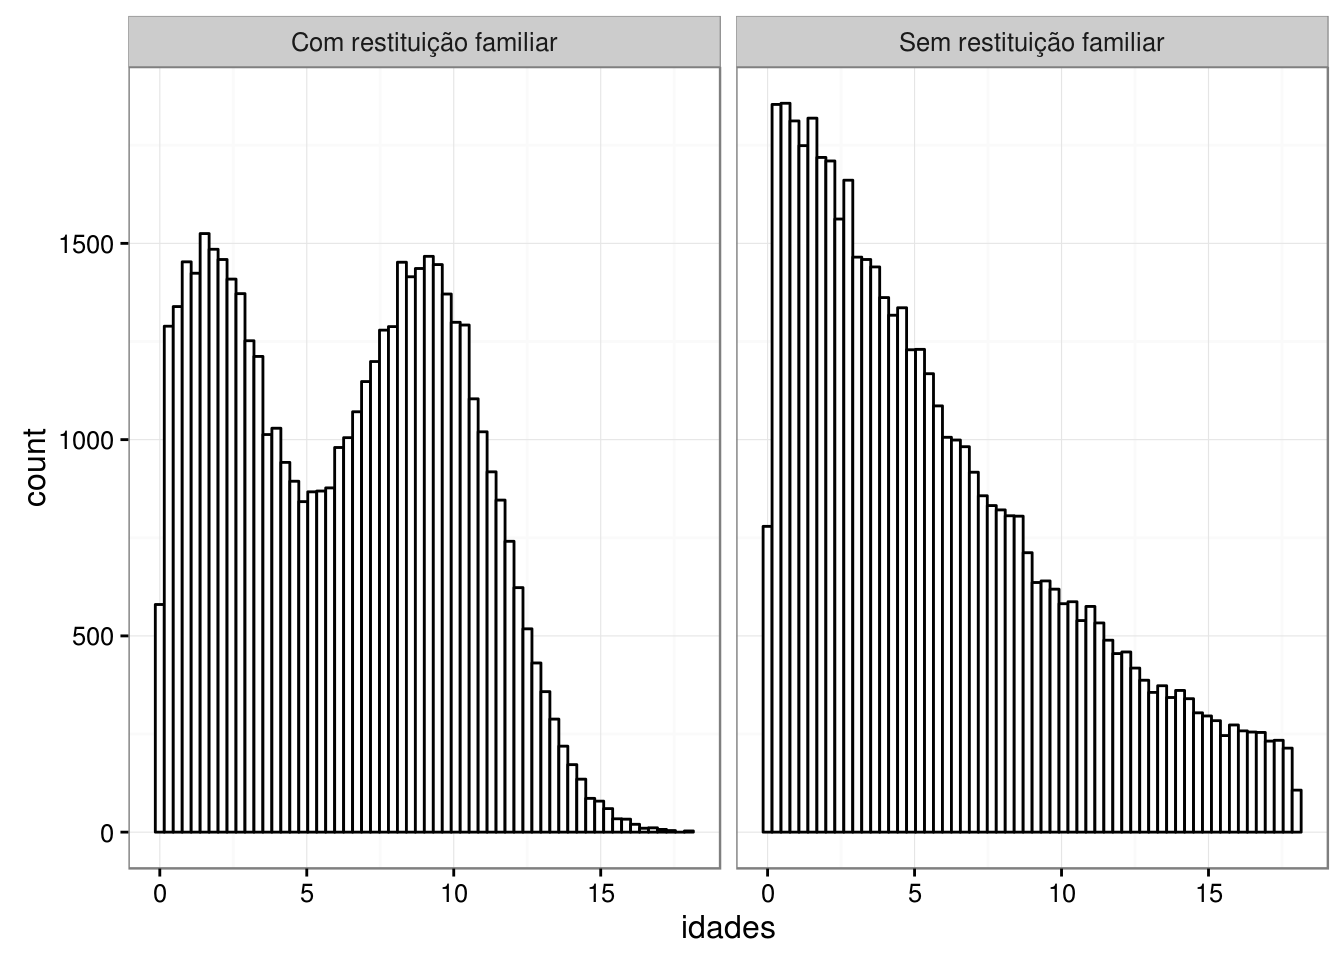
\includegraphics{curso-jurimetria_files/figure-latex/unnamed-chunk-68-1} \end{center}

Note que, como cada uma destas distriuições está associada a uma causa
de cadastro no CNA, vamos incluir a proporção de crianças registradas
devido a processos de restituição familiar como um parâmetro do modelo.
Por simplicidade, fixaremos este valor em 15\%, equivalente à proporção
observada no relatório supra citado.

O impacto de variações na distribuição de idades das crianças
cadastradas no CNA será resumido no parâmetro que controla a localização
da segunda ``corcova'' da distribuição de idades das crianças
cadastradas no CNA após processos com restituição familiar.

Por fim, precisamos fixar os valores de \(K\) e \(P\). Para isso,
fixaremos a razão \(\frac{K}{P}\) em \(3,52\), pois este número
representa a razão do número total de crianças cadastradas no CNA,
ativas ou inativas, pelo número total de pretendentes cadastrados no
CNA, ativos ou inativos. Como \(P=3,52K\), vamos nos preocupar apenas
variar o parâmetro \(K\).

\subsection{Implementação}\label{implementacao-1}

As simulações propriamente ditas serão realizadas utilizando programas
desenvolvidos no software R.

Em linhas gerais, a implementação utilizará dois vetores. Um deles
conterá as idades das crianças cadastradas e o outro conterá as idades
máximas preferidas por cada pretendente cadastrado. A cada iteração, o
vetor das crianças é atualizado retirando as crianças que foram adotadas
ou que atingiram a maioridade e adicionando as novas crianças
cadastradas no CNA. O vetor dos pretendentes é atualizado retirando
aqueles que adotaram alguma criança e adicionando nos novos cadastrados.

Primeiramente, construíremos funções que sorteiem as idades das crianças
que são registradas no CNA e preferências dos pretendenentes registrados
no CNA.

\begin{Shaded}
\begin{Highlighting}[]
\CommentTok{#Sorteia n_pretendentes a partir de uma distribuição desejada. Por default, utiliza a distribuição disponível no relatório sobre adoção.}

\NormalTok{distr <-}\StringTok{ }\KeywordTok{c}\NormalTok{(}\FloatTok{0.1478}\NormalTok{,}\FloatTok{0.1833}\NormalTok{,}\FloatTok{0.1974}\NormalTok{,}\FloatTok{0.1879}\NormalTok{,}\FloatTok{0.1056}\NormalTok{,}\FloatTok{0.0981}\NormalTok{,}\FloatTok{0.0362}\NormalTok{,}
           \FloatTok{0.0176}\NormalTok{,}\FloatTok{0.0095}\NormalTok{,}\FloatTok{0.0032}\NormalTok{,}\FloatTok{0.0066}\NormalTok{,}\FloatTok{0.0015}\NormalTok{,}\FloatTok{0.0020}\NormalTok{,}\FloatTok{0.0007}\NormalTok{,}
           \FloatTok{0.0005}\NormalTok{,}\FloatTok{0.0006}\NormalTok{,}\FloatTok{0.0003}\NormalTok{,}\FloatTok{0.0012}\NormalTok{)}
\NormalTok{sorteia_preferencias <-}\StringTok{ }\NormalTok{function(n_pretendentes, }\DataTypeTok{distribuicao =} \NormalTok{distr)\{}
  \KeywordTok{sapply}\NormalTok{(}\KeywordTok{runif}\NormalTok{(n_pretendentes), function(x) \{}\KeywordTok{which.max}\NormalTok{(x <}\StringTok{ }\NormalTok{distribuicao) -}\StringTok{ }\DecValTok{1}\NormalTok{\})}
\NormalTok{\}}

\CommentTok{#Sorteia n valores de uma mistura de normais limitada ao intervalo de 0 a 18.}

\NormalTok{tnorMix <-}\StringTok{ }\NormalTok{function(n,fit)\{}
  \NormalTok{x <-}\StringTok{ }\NormalTok{nor1mix::}\KeywordTok{rnorMix}\NormalTok{(n,fit)}
  \NormalTok{while(x <}\StringTok{ }\DecValTok{0} \NormalTok{|}\StringTok{ }\NormalTok{x >}\StringTok{ }\DecValTok{18}\NormalTok{)\{}
    \NormalTok{x <-}\StringTok{ }\NormalTok{nor1mix::}\KeywordTok{rnorMix}\NormalTok{(n,fit)}
  \NormalTok{\}}
  \KeywordTok{return}\NormalTok{(x)}
\NormalTok{\}}

\CommentTok{#Sorteia n valores de uma distribuição gama limitada ao intervalo de 0 a 18.}

\NormalTok{trgamma <-}\StringTok{ }\NormalTok{function(n,shape,rate)\{}
  \NormalTok{x <-}\StringTok{ }\KeywordTok{rgamma}\NormalTok{(n,shape,rate)}
  \NormalTok{while(x <}\StringTok{ }\DecValTok{0} \NormalTok{|}\StringTok{ }\NormalTok{x >}\StringTok{ }\DecValTok{18}\NormalTok{)\{}
    \NormalTok{x <-}\StringTok{ }\KeywordTok{rgamma}\NormalTok{(n,shape,rate)}
  \NormalTok{\}}
  \KeywordTok{return}\NormalTok{(x)}
\NormalTok{\}}

\CommentTok{#Sorteia as idades de n_criancas_para_adocao a partir das distribuições acima, utilizando um conjunto de parâmetros.}

\NormalTok{sorteia_idades <-}\StringTok{ }\NormalTok{function(n_criancas_para_adocao, shape, rate, mu1, mu2, sigma, p, }\DataTypeTok{peso =} \FloatTok{0.5}\NormalTok{)\{}
  \NormalTok{distr <-}\StringTok{ }\NormalTok{nor1mix::}\KeywordTok{norMix}\NormalTok{(}\DataTypeTok{mu =} \KeywordTok{c}\NormalTok{(mu1,mu2), }\DataTypeTok{sigma =} \KeywordTok{rep}\NormalTok{(sigma,}\DecValTok{2}\NormalTok{), }\DataTypeTok{w =} \KeywordTok{c}\NormalTok{(}\DecValTok{1}\NormalTok{-peso,peso))}
  \KeywordTok{sapply}\NormalTok{(}\KeywordTok{runif}\NormalTok{(n_criancas_para_adocao), function(x)\{}\KeywordTok{ifelse}\NormalTok{(x <}\StringTok{ }\NormalTok{p, }\KeywordTok{ifelse}\NormalTok{(}\KeywordTok{runif}\NormalTok{(}\DecValTok{1}\NormalTok{) <}\StringTok{ }\FloatTok{0.5}\NormalTok{,}\KeywordTok{trgamma}\NormalTok{(}\DecValTok{1}\NormalTok{,shape,rate),}\KeywordTok{rexp}\NormalTok{(}\DecValTok{1}\NormalTok{)), }\KeywordTok{tnorMix}\NormalTok{(}\DecValTok{1}\NormalTok{,distr))\})}
\NormalTok{\}}
\end{Highlighting}
\end{Shaded}

A partir dessas funções, podemos inicializar os nossos vetores:

As listas inicializadas seguem abaixo

\begin{longtable}[]{@{}cc@{}}
\caption{Exemplo de conjunto de crianças simulado}\tabularnewline
\toprule
\begin{minipage}[b]{0.13\columnwidth}\centering\strut
idades
\strut\end{minipage} &
\begin{minipage}[b]{0.05\columnwidth}\centering\strut
id
\strut\end{minipage}\tabularnewline
\midrule
\endfirsthead
\toprule
\begin{minipage}[b]{0.13\columnwidth}\centering\strut
idades
\strut\end{minipage} &
\begin{minipage}[b]{0.05\columnwidth}\centering\strut
id
\strut\end{minipage}\tabularnewline
\midrule
\endhead
\begin{minipage}[t]{0.13\columnwidth}\centering\strut
0.2006772
\strut\end{minipage} &
\begin{minipage}[t]{0.05\columnwidth}\centering\strut
1
\strut\end{minipage}\tabularnewline
\begin{minipage}[t]{0.13\columnwidth}\centering\strut
9.7013161
\strut\end{minipage} &
\begin{minipage}[t]{0.05\columnwidth}\centering\strut
2
\strut\end{minipage}\tabularnewline
\begin{minipage}[t]{0.13\columnwidth}\centering\strut
3.6083768
\strut\end{minipage} &
\begin{minipage}[t]{0.05\columnwidth}\centering\strut
3
\strut\end{minipage}\tabularnewline
\begin{minipage}[t]{0.13\columnwidth}\centering\strut
2.0634004
\strut\end{minipage} &
\begin{minipage}[t]{0.05\columnwidth}\centering\strut
4
\strut\end{minipage}\tabularnewline
\begin{minipage}[t]{0.13\columnwidth}\centering\strut
4.1576919
\strut\end{minipage} &
\begin{minipage}[t]{0.05\columnwidth}\centering\strut
5
\strut\end{minipage}\tabularnewline
\begin{minipage}[t]{0.13\columnwidth}\centering\strut
1.5176869
\strut\end{minipage} &
\begin{minipage}[t]{0.05\columnwidth}\centering\strut
6
\strut\end{minipage}\tabularnewline
\begin{minipage}[t]{0.13\columnwidth}\centering\strut
5.6406676
\strut\end{minipage} &
\begin{minipage}[t]{0.05\columnwidth}\centering\strut
7
\strut\end{minipage}\tabularnewline
\begin{minipage}[t]{0.13\columnwidth}\centering\strut
3.2431550
\strut\end{minipage} &
\begin{minipage}[t]{0.05\columnwidth}\centering\strut
8
\strut\end{minipage}\tabularnewline
\begin{minipage}[t]{0.13\columnwidth}\centering\strut
5.6340124
\strut\end{minipage} &
\begin{minipage}[t]{0.05\columnwidth}\centering\strut
9
\strut\end{minipage}\tabularnewline
\begin{minipage}[t]{0.13\columnwidth}\centering\strut
4.5060209
\strut\end{minipage} &
\begin{minipage}[t]{0.05\columnwidth}\centering\strut
10
\strut\end{minipage}\tabularnewline
\bottomrule
\end{longtable}

\begin{longtable}[]{@{}cc@{}}
\caption{Exemplo de conjunto de pretendentes simulado}\tabularnewline
\toprule
\begin{minipage}[b]{0.33\columnwidth}\centering\strut
idade\_maxima\_preferida
\strut\end{minipage} &
\begin{minipage}[b]{0.05\columnwidth}\centering\strut
id
\strut\end{minipage}\tabularnewline
\midrule
\endfirsthead
\toprule
\begin{minipage}[b]{0.33\columnwidth}\centering\strut
idade\_maxima\_preferida
\strut\end{minipage} &
\begin{minipage}[b]{0.05\columnwidth}\centering\strut
id
\strut\end{minipage}\tabularnewline
\midrule
\endhead
\begin{minipage}[t]{0.33\columnwidth}\centering\strut
0
\strut\end{minipage} &
\begin{minipage}[t]{0.05\columnwidth}\centering\strut
1
\strut\end{minipage}\tabularnewline
\begin{minipage}[t]{0.33\columnwidth}\centering\strut
0
\strut\end{minipage} &
\begin{minipage}[t]{0.05\columnwidth}\centering\strut
2
\strut\end{minipage}\tabularnewline
\begin{minipage}[t]{0.33\columnwidth}\centering\strut
0
\strut\end{minipage} &
\begin{minipage}[t]{0.05\columnwidth}\centering\strut
3
\strut\end{minipage}\tabularnewline
\begin{minipage}[t]{0.33\columnwidth}\centering\strut
0
\strut\end{minipage} &
\begin{minipage}[t]{0.05\columnwidth}\centering\strut
4
\strut\end{minipage}\tabularnewline
\begin{minipage}[t]{0.33\columnwidth}\centering\strut
0
\strut\end{minipage} &
\begin{minipage}[t]{0.05\columnwidth}\centering\strut
5
\strut\end{minipage}\tabularnewline
\begin{minipage}[t]{0.33\columnwidth}\centering\strut
0
\strut\end{minipage} &
\begin{minipage}[t]{0.05\columnwidth}\centering\strut
6
\strut\end{minipage}\tabularnewline
\begin{minipage}[t]{0.33\columnwidth}\centering\strut
0
\strut\end{minipage} &
\begin{minipage}[t]{0.05\columnwidth}\centering\strut
7
\strut\end{minipage}\tabularnewline
\begin{minipage}[t]{0.33\columnwidth}\centering\strut
0
\strut\end{minipage} &
\begin{minipage}[t]{0.05\columnwidth}\centering\strut
8
\strut\end{minipage}\tabularnewline
\begin{minipage}[t]{0.33\columnwidth}\centering\strut
0
\strut\end{minipage} &
\begin{minipage}[t]{0.05\columnwidth}\centering\strut
9
\strut\end{minipage}\tabularnewline
\begin{minipage}[t]{0.33\columnwidth}\centering\strut
0
\strut\end{minipage} &
\begin{minipage}[t]{0.05\columnwidth}\centering\strut
10
\strut\end{minipage}\tabularnewline
\bottomrule
\end{longtable}

Para completar a inicialização e finalizar a implementação, precisamos
desenvolver um algoritmo que maximize o número de matchs a partir de um
conjunto de idades e preferências. O algoritmo abaixo cumpre esse papel,
realizando uma varredura das idades ordenadas para checar a viabilidade
da adoção de cada criança.

\begin{Shaded}
\begin{Highlighting}[]
  \CommentTok{# Arredonda a idade das crianças cadastradas para baixo e ordena as idades arredondadas em ordem decrescente.}
  \NormalTok{criancas_floor <-}\StringTok{ }\KeywordTok{floor}\NormalTok{(}\KeywordTok{sort}\NormalTok{(idades, }\DataTypeTok{decreasing =} \NormalTok{T))}

  \CommentTok{# Ordena as idades máximas preferidas de cada pretendente em ordem decrescente.}
  \NormalTok{pretendentes <-}\StringTok{ }\KeywordTok{sort}\NormalTok{(pretendentes, }\DataTypeTok{decreasing =} \NormalTok{T)}
  
  \CommentTok{# Ordena a idade das crianças cadastradas em ordem decrescente.}
  \NormalTok{criancas <-}\StringTok{ }\KeywordTok{sort}\NormalTok{(idades, }\DataTypeTok{decreasing =} \NormalTok{T)}

  \CommentTok{# Contador que percorre o vetor de idades.}
  \NormalTok{i =}\StringTok{ }\DecValTok{1}
  
  \CommentTok{# Inicialização do número de pareamentos.}
  \NormalTok{num_match =}\StringTok{ }\DecValTok{0}
  
  \NormalTok{while(i <=}\StringTok{ }\KeywordTok{length}\NormalTok{(criancas))\{}

    \CommentTok{#Se a idade arredondada da criança de maior idade for menor que a maior idade máxima tolerada por um pretendente, um pareamento é possível. }
    \NormalTok{if(criancas_floor[i] <=}\StringTok{ }\NormalTok{pretendentes[}\DecValTok{1}\NormalTok{])\{}

      \CommentTok{#Remove a criança adotada do vetor de crianças}
      \NormalTok{criancas <-}\StringTok{ }\NormalTok{criancas[-i]}
      
      \CommentTok{#Remove a criança adotada do vetor de idades arredondadas}
      \NormalTok{criancas_floor <-}\StringTok{ }\NormalTok{criancas_floor[-i]}

      \CommentTok{#Remove o pretendente que adotou a criança dos pretendentes disponíveis}
      \NormalTok{pretendentes <-}\StringTok{ }\NormalTok{pretendentes[-}\DecValTok{1}\NormalTok{]}
      
      \CommentTok{#Conta um novo pareamento}
      \NormalTok{num_match =}\StringTok{ }\NormalTok{num_match +}\StringTok{ }\DecValTok{1}
      
      \CommentTok{#O contador recua uma posição por conta da remoção da criança adotada}
      \NormalTok{i <-}\StringTok{ }\NormalTok{i}\DecValTok{-1}
    \NormalTok{\}}
    
    \CommentTok{#Continua a contagem}
    \NormalTok{i <-}\StringTok{ }\NormalTok{i +}\StringTok{ }\DecValTok{1}
  \NormalTok{\}}
\end{Highlighting}
\end{Shaded}

Na verdade, este algoritmo pode ser melhorado se realizarmos uma
adaptação na regra de pareamento. Não é necessário que a criança de
maior idade seja pareada com o pretendente de maior idade máxima
tolerada. Embora seja improvável, essa regra de pareamento pode produzir
a adoção de uma criança de 10 anos por um pretendente que não se opõe a
adotar jovens de até 17 anos. De certa forma, este tipo de pareamento é
um ``desperdício'', já que pretendentes com idades máximas toleradas
grandes são mais raros, de forma que é mais interessante pareá-los com
jovens mais velhos.

A adaptação sugerida no parágrafo anterior pode ser implementada da
forma que segue, notando que, na função, as duas estratégias estão
disponíveis na simulação através do parâmetro ``tipo''.

\begin{Shaded}
\begin{Highlighting}[]
\NormalTok{matching <-}\StringTok{ }\NormalTok{function(pretendentes, criancas, }\DataTypeTok{tipo =} \DecValTok{1}\NormalTok{)\{}

  \NormalTok{criancas_floor <-}\StringTok{ }\KeywordTok{floor}\NormalTok{(}\KeywordTok{sort}\NormalTok{(criancas, }\DataTypeTok{decreasing =} \NormalTok{T))}
  \NormalTok{pretendentes <-}\StringTok{ }\KeywordTok{sort}\NormalTok{(pretendentes, }\DataTypeTok{decreasing =} \NormalTok{T)}
  \NormalTok{criancas <-}\StringTok{ }\KeywordTok{sort}\NormalTok{(criancas, }\DataTypeTok{decreasing =} \NormalTok{T)}

  \NormalTok{i =}\StringTok{ }\DecValTok{1}
  \NormalTok{num_match =}\StringTok{ }\DecValTok{0}
  \NormalTok{while(i <=}\StringTok{ }\KeywordTok{length}\NormalTok{(criancas))\{}

    \NormalTok{if(criancas_floor[i] <=}\StringTok{ }\NormalTok{pretendentes[}\DecValTok{1}\NormalTok{])\{}

      \NormalTok{j =}\StringTok{ }\DecValTok{1}

      \NormalTok{while(tipo ==}\StringTok{ }\DecValTok{2} \NormalTok{&}\StringTok{ }\NormalTok{j !=}\StringTok{ }\KeywordTok{length}\NormalTok{(pretendentes) &}\StringTok{ }\NormalTok{criancas_floor[i]<=pretendentes[}\KeywordTok{ifelse}\NormalTok{(j <}\StringTok{ }\KeywordTok{length}\NormalTok{(pretendentes), j}\DecValTok{+1}\NormalTok{, }\KeywordTok{length}\NormalTok{(pretendentes))])\{}
        \NormalTok{j =}\StringTok{ }\NormalTok{j +}\StringTok{ }\DecValTok{1}
      \NormalTok{\}}

      \NormalTok{criancas <-}\StringTok{ }\NormalTok{criancas[-i]}
      \NormalTok{criancas_floor <-}\StringTok{ }\NormalTok{criancas_floor[-i]}

      \NormalTok{pretendentes <-}\StringTok{ }\NormalTok{pretendentes[-j]}
      \NormalTok{num_match =}\StringTok{ }\NormalTok{num_match +}\StringTok{ }\DecValTok{1}
      \NormalTok{i <-}\StringTok{ }\NormalTok{i}\DecValTok{-1}
    \NormalTok{\}}
    \NormalTok{i <-}\StringTok{ }\NormalTok{i +}\StringTok{ }\DecValTok{1}
  \NormalTok{\}}

  \KeywordTok{return}\NormalTok{(}\KeywordTok{list}\NormalTok{(criancas,pretendentes, num_match))}
\NormalTok{\}}
\end{Highlighting}
\end{Shaded}

O exemplo abaixo ilustra o funcionamento dessas estratégias de
pareamento.

\begin{Shaded}
\begin{Highlighting}[]
\NormalTok{p <-}\StringTok{ }\KeywordTok{sorteia_preferencias}\NormalTok{(}\DecValTok{30}\NormalTok{)}
\NormalTok{idades <-}\StringTok{ }\KeywordTok{sorteia_idades}\NormalTok{(}\DecValTok{30}\NormalTok{, }\FloatTok{1.1}\NormalTok{, }\FloatTok{0.15}\NormalTok{, }\DecValTok{1}\NormalTok{, }\DecValTok{9}\NormalTok{, }\FloatTok{2.8}\NormalTok{, }\FloatTok{0.1}\NormalTok{, }\FloatTok{0.5}\NormalTok{)}

\KeywordTok{print}\NormalTok{(}\KeywordTok{sort}\NormalTok{(}\KeywordTok{round}\NormalTok{(idades, }\DecValTok{2}\NormalTok{), }\DataTypeTok{decreasing =} \NormalTok{T))}
\end{Highlighting}
\end{Shaded}

\begin{verbatim}
##  [1] 13.22 12.96 12.72 12.41 10.82 10.44  9.79  9.30  8.93  8.71  7.30
## [12]  7.13  7.03  6.66  6.59  6.51  5.29  4.98  4.66  3.55  3.32  3.01
## [23]  2.72  2.14  1.31  1.21  1.09  0.65  0.42  0.42
\end{verbatim}

\begin{Shaded}
\begin{Highlighting}[]
\KeywordTok{print}\NormalTok{(}\KeywordTok{sort}\NormalTok{(}\KeywordTok{round}\NormalTok{(p, }\DecValTok{2}\NormalTok{), }\DataTypeTok{decreasing =} \NormalTok{T))}
\end{Highlighting}
\end{Shaded}

\begin{verbatim}
##  [1] 2 1 1 1 0 0 0 0 0 0 0 0 0 0 0 0 0 0 0 0 0 0 0 0 0 0 0 0 0 0
\end{verbatim}

\begin{Shaded}
\begin{Highlighting}[]
\CommentTok{#Lista contendo o vetor de crianças e de pretendentes restantes.}
\NormalTok{pareamentos_estrategia_1 <-}\StringTok{ }\KeywordTok{matching}\NormalTok{(p, idades, }\DecValTok{1}\NormalTok{)}
\NormalTok{pareamentos_estrategia_2 <-}\StringTok{ }\KeywordTok{matching}\NormalTok{(p, idades, }\DecValTok{2}\NormalTok{)}

\KeywordTok{print}\NormalTok{(pareamentos_estrategia_1)}
\end{Highlighting}
\end{Shaded}

\begin{verbatim}
## [[1]]
##  [1] 13.220144 12.963619 12.720426 12.409301 10.816369 10.435139  9.794466
##  [8]  9.298955  8.934183  8.711584  7.295204  7.132229  7.025862  6.656854
## [15]  6.590421  6.507732  5.285900  4.983965  4.661280  3.550157  3.320593
## [22]  3.011672  2.139547
## 
## [[2]]
##  [1] 0 0 0 0 0 0 0 0 0 0 0 0 0 0 0 0 0 0 0 0 0 0 0
## 
## [[3]]
## [1] 7
\end{verbatim}

\begin{Shaded}
\begin{Highlighting}[]
\KeywordTok{print}\NormalTok{(pareamentos_estrategia_2)}
\end{Highlighting}
\end{Shaded}

\begin{verbatim}
## [[1]]
##  [1] 13.220144 12.963619 12.720426 12.409301 10.816369 10.435139  9.794466
##  [8]  9.298955  8.934183  8.711584  7.295204  7.132229  7.025862  6.656854
## [15]  6.590421  6.507732  5.285900  4.983965  4.661280  3.550157  3.320593
## [22]  3.011672  2.139547
## 
## [[2]]
##  [1] 0 0 0 0 0 0 0 0 0 0 0 0 0 0 0 0 0 0 0 0 0 0 0
## 
## [[3]]
## [1] 7
\end{verbatim}

\subsection{Análise dos resultados}\label{analise-dos-resultados-1}

Antes de proceder com a análise de resultados vamos responder às
perguntas propostas anteriormente:

\begin{enumerate}
\def\labelenumi{\arabic{enumi}.}
\tightlist
\item
  Desejamos analisar o impacto de quais parâmetros?
\end{enumerate}

A idade de entrada das crianças no CNA e as estratégias de pareamento de
crianças e pretendentes.

\begin{enumerate}
\def\labelenumi{\arabic{enumi}.}
\setcounter{enumi}{1}
\tightlist
\item
  Quais são as variáveis sobre as quais desejamos analisar o impacto?
\end{enumerate}

Desejamos a variação do número de crianças que atingem a maioridade ao
longo do tempo, o número de crianças e pretendentes disponíveis e o
número de adoções.

\begin{enumerate}
\def\labelenumi{\arabic{enumi}.}
\setcounter{enumi}{2}
\tightlist
\item
  O que a alteração dos parâmetros de interesse deve causar em cada
  variável?
\end{enumerate}

Espera-se que uma menor idade de regitro no CNA diminua o número de
crianças que atingem a maioridade, aumente o número de adoções e,
consequentemente, diminuia o número de crianças disponíveis para adoção.
Temos interesse especial em avaliar o tamanho dessas
diminuições/acréscimos.

\subsubsection{Idade de entrada no CNA}\label{idade-de-entrada-no-cna}

Desejamos checar se, conforme a idade de entrada no CNA diminui, o
número de maiores de idade por iteração fica menor. Este é o caso, como
se observa na figura abaixo.

\begin{Shaded}
\begin{Highlighting}[]
\NormalTok{maiores_de_idade <-}\StringTok{ }\NormalTok{function(}\DataTypeTok{tipo =} \DecValTok{1}\NormalTok{, }\DataTypeTok{tempos =} \DecValTok{1}\NormalTok{:}\DecValTok{10}\NormalTok{, }\DataTypeTok{K =} \DecValTok{100}\NormalTok{, }\DataTypeTok{p_cada_tipo =} \FloatTok{0.1}\NormalTok{, }\DataTypeTok{unidade =} \DecValTok{1}\NormalTok{, }\DataTypeTok{idade_maxima =} \DecValTok{9}\NormalTok{)\{}
    \KeywordTok{realiza_processo}\NormalTok{(tipo, tempos, K, p_cada_tipo, unidade, idade_maxima)$maiores_de_idade}
\NormalTok{\}}

\KeywordTok{expand.grid}\NormalTok{(}\DataTypeTok{K =} \KeywordTok{c}\NormalTok{(}\DecValTok{100}\NormalTok{,}\DecValTok{200}\NormalTok{,}\DecValTok{300}\NormalTok{), }\DataTypeTok{idade_maxima =} \DecValTok{7}\NormalTok{:}\DecValTok{9}\NormalTok{) %>%}\StringTok{    }\NormalTok{plyr:::}\KeywordTok{mdply}\NormalTok{(maiores_de_idade, }\DataTypeTok{tempo =} \DecValTok{1}\NormalTok{:}\DecValTok{20}\NormalTok{) %>%}\StringTok{ }
\StringTok{  }\NormalTok{reshape2::}\KeywordTok{melt}\NormalTok{(}\DataTypeTok{id.vars =} \KeywordTok{c}\NormalTok{(}\StringTok{'K'}\NormalTok{,}\StringTok{'idade_maxima'}\NormalTok{)) %>%}\StringTok{ }
\StringTok{  }\KeywordTok{select}\NormalTok{(-variable) %>%}\StringTok{ }
\StringTok{  }\KeywordTok{group_by}\NormalTok{(K, idade_maxima) %>%}\StringTok{ }
\StringTok{  }\KeywordTok{mutate}\NormalTok{(}\DataTypeTok{periodo =} \DecValTok{1}\NormalTok{:}\KeywordTok{n}\NormalTok{()) %>%}
\StringTok{  }\KeywordTok{ungroup}\NormalTok{() %>%}\StringTok{ }
\StringTok{  }\KeywordTok{mutate}\NormalTok{(}\DataTypeTok{idade_maxima =} \KeywordTok{paste0}\NormalTok{(idade_maxima,}\StringTok{' anos'}\NormalTok{)) %>%}\StringTok{ }
\StringTok{  }\KeywordTok{ggplot}\NormalTok{(}\KeywordTok{aes}\NormalTok{(}\DataTypeTok{x =} \NormalTok{periodo, }\DataTypeTok{y =} \NormalTok{value, }\DataTypeTok{color =} \NormalTok{idade_maxima))+}
\StringTok{    }\KeywordTok{geom_line}\NormalTok{()+}
\StringTok{    }\KeywordTok{facet_grid}\NormalTok{(K ~}\StringTok{ }\NormalTok{idade_maxima)+}
\StringTok{  }\KeywordTok{theme_bw}\NormalTok{()+}
\StringTok{  }\KeywordTok{xlab}\NormalTok{(}\StringTok{'Iteração'}\NormalTok{)+}
\StringTok{  }\KeywordTok{ylab}\NormalTok{(}\StringTok{'Número de maiores de idade'}\NormalTok{)}
\end{Highlighting}
\end{Shaded}

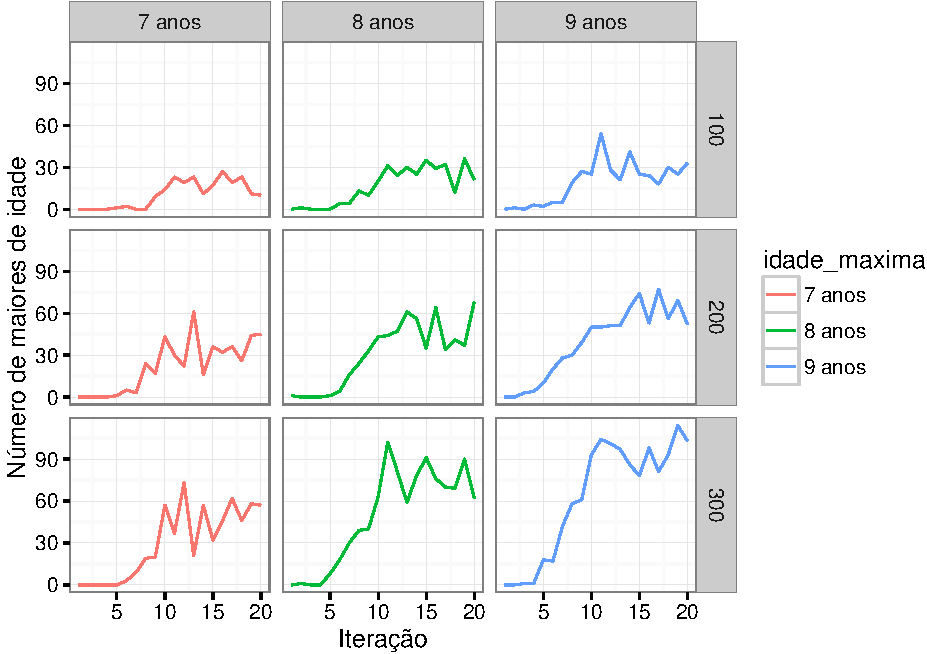
\includegraphics{curso-jurimetria_files/figure-latex/unnamed-chunk-76-1.pdf}

A diminuição no número de maiores de idade implica em mais crianças
sendo adotadas ao longo do tempo, de forma que devemos verificar uma
diminuição nesta variável também. O resultado deste teste segue na
figura abaixo.

\begin{Shaded}
\begin{Highlighting}[]
\NormalTok{criancas_disponiveis <-}\StringTok{ }\NormalTok{function(}\DataTypeTok{tipo =} \DecValTok{1}\NormalTok{, }\DataTypeTok{tempos =} \DecValTok{1}\NormalTok{:}\DecValTok{10}\NormalTok{, }\DataTypeTok{K =} \DecValTok{100}\NormalTok{, }\DataTypeTok{p_cada_tipo =} \FloatTok{0.1}\NormalTok{, }\DataTypeTok{unidade =} \DecValTok{1}\NormalTok{, }\DataTypeTok{idade_maxima =} \DecValTok{9}\NormalTok{)\{}
    \KeywordTok{realiza_processo}\NormalTok{(tipo, tempos, K, p_cada_tipo, unidade, idade_maxima)$criancas_disponiveis}
\NormalTok{\}}

\KeywordTok{expand.grid}\NormalTok{(}\DataTypeTok{K =} \KeywordTok{c}\NormalTok{(}\DecValTok{100}\NormalTok{,}\DecValTok{200}\NormalTok{,}\DecValTok{300}\NormalTok{), }\DataTypeTok{idade_maxima =} \DecValTok{7}\NormalTok{:}\DecValTok{9}\NormalTok{) %>%}\StringTok{    }\NormalTok{plyr:::}\KeywordTok{mdply}\NormalTok{(criancas_disponiveis, }\DataTypeTok{tempo =} \DecValTok{1}\NormalTok{:}\DecValTok{20}\NormalTok{) %>%}\StringTok{ }
\StringTok{  }\NormalTok{reshape2::}\KeywordTok{melt}\NormalTok{(}\DataTypeTok{id.vars =} \KeywordTok{c}\NormalTok{(}\StringTok{'K'}\NormalTok{,}\StringTok{'idade_maxima'}\NormalTok{)) %>%}\StringTok{ }
\StringTok{  }\KeywordTok{select}\NormalTok{(-variable) %>%}\StringTok{ }
\StringTok{  }\KeywordTok{group_by}\NormalTok{(K, idade_maxima) %>%}\StringTok{ }
\StringTok{  }\KeywordTok{mutate}\NormalTok{(}\DataTypeTok{periodo =} \DecValTok{1}\NormalTok{:}\KeywordTok{n}\NormalTok{()) %>%}
\StringTok{  }\KeywordTok{ungroup}\NormalTok{() %>%}\StringTok{ }
\StringTok{  }\KeywordTok{mutate}\NormalTok{(}\DataTypeTok{idade_maxima =} \KeywordTok{paste0}\NormalTok{(idade_maxima,}\StringTok{' anos'}\NormalTok{)) %>%}\StringTok{ }
\StringTok{  }\KeywordTok{ggplot}\NormalTok{(}\KeywordTok{aes}\NormalTok{(}\DataTypeTok{x =} \NormalTok{periodo, }\DataTypeTok{y =} \NormalTok{value, }\DataTypeTok{color =} \NormalTok{idade_maxima))+}
\StringTok{    }\KeywordTok{geom_line}\NormalTok{()+}
\StringTok{    }\KeywordTok{facet_grid}\NormalTok{(K ~}\StringTok{ }\NormalTok{idade_maxima)+}
\StringTok{  }\KeywordTok{theme_bw}\NormalTok{()+}
\StringTok{  }\KeywordTok{xlab}\NormalTok{(}\StringTok{'Iteração'}\NormalTok{)+}
\StringTok{  }\KeywordTok{ylab}\NormalTok{(}\StringTok{'Número de crianças disponíveis para adoção'}\NormalTok{)}
\end{Highlighting}
\end{Shaded}

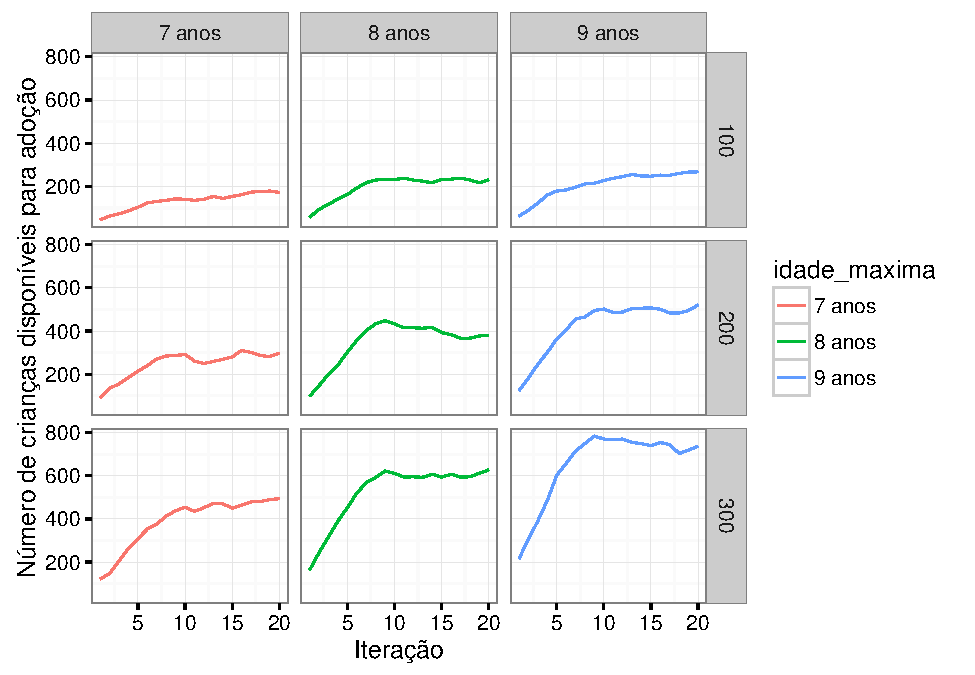
\includegraphics{curso-jurimetria_files/figure-latex/unnamed-chunk-77-1.pdf}

Por fim, uma diminuição na idade das crianças cadastradas no CNA deve
favorecer a ocorrência de um maior número de pareamentos entre
pretendentes e crianças, considerando que grande parte dos pretendentes
prefere crianças mais jovens.

\begin{Shaded}
\begin{Highlighting}[]
\NormalTok{numero_de_pareamentos <-}\StringTok{ }\NormalTok{function(}\DataTypeTok{tipo =} \DecValTok{1}\NormalTok{, }\DataTypeTok{tempos =} \DecValTok{1}\NormalTok{:}\DecValTok{10}\NormalTok{, }\DataTypeTok{K =} \DecValTok{100}\NormalTok{, }\DataTypeTok{p_cada_tipo =} \FloatTok{0.1}\NormalTok{, }\DataTypeTok{unidade =} \DecValTok{1}\NormalTok{, }\DataTypeTok{idade_maxima =} \DecValTok{9}\NormalTok{)\{}
    \KeywordTok{realiza_processo}\NormalTok{(tipo, tempos, K, p_cada_tipo, unidade, idade_maxima)$numero_de_pareamentos}
\NormalTok{\}}

\KeywordTok{expand.grid}\NormalTok{(}\DataTypeTok{K =} \KeywordTok{c}\NormalTok{(}\DecValTok{100}\NormalTok{,}\DecValTok{200}\NormalTok{,}\DecValTok{300}\NormalTok{), }\DataTypeTok{idade_maxima =} \DecValTok{7}\NormalTok{:}\DecValTok{9}\NormalTok{) %>%}\StringTok{    }\NormalTok{plyr:::}\KeywordTok{mdply}\NormalTok{(numero_de_pareamentos, }\DataTypeTok{tempo =} \DecValTok{1}\NormalTok{:}\DecValTok{20}\NormalTok{) %>%}\StringTok{ }
\StringTok{  }\NormalTok{reshape2::}\KeywordTok{melt}\NormalTok{(}\DataTypeTok{id.vars =} \KeywordTok{c}\NormalTok{(}\StringTok{'K'}\NormalTok{,}\StringTok{'idade_maxima'}\NormalTok{)) %>%}\StringTok{ }
\StringTok{  }\KeywordTok{select}\NormalTok{(-variable) %>%}\StringTok{ }
\StringTok{  }\KeywordTok{group_by}\NormalTok{(K, idade_maxima) %>%}\StringTok{ }
\StringTok{  }\KeywordTok{mutate}\NormalTok{(}\DataTypeTok{periodo =} \DecValTok{1}\NormalTok{:}\KeywordTok{n}\NormalTok{()) %>%}
\StringTok{  }\KeywordTok{ungroup}\NormalTok{() %>%}\StringTok{ }
\StringTok{  }\KeywordTok{mutate}\NormalTok{(}\DataTypeTok{idade_maxima =} \KeywordTok{paste0}\NormalTok{(idade_maxima,}\StringTok{' anos'}\NormalTok{)) %>%}\StringTok{ }
\StringTok{  }\KeywordTok{ggplot}\NormalTok{(}\KeywordTok{aes}\NormalTok{(}\DataTypeTok{x =} \NormalTok{periodo, }\DataTypeTok{y =} \NormalTok{value, }\DataTypeTok{color =} \NormalTok{idade_maxima))+}
\StringTok{    }\KeywordTok{geom_line}\NormalTok{()+}
\StringTok{    }\KeywordTok{facet_grid}\NormalTok{(K ~}\StringTok{ }\NormalTok{idade_maxima)+}
\StringTok{  }\KeywordTok{theme_bw}\NormalTok{()+}
\StringTok{  }\KeywordTok{xlab}\NormalTok{(}\StringTok{'Iteração'}\NormalTok{)+}
\StringTok{  }\KeywordTok{ylab}\NormalTok{(}\StringTok{'Número de pareamentos'}\NormalTok{)}
\end{Highlighting}
\end{Shaded}

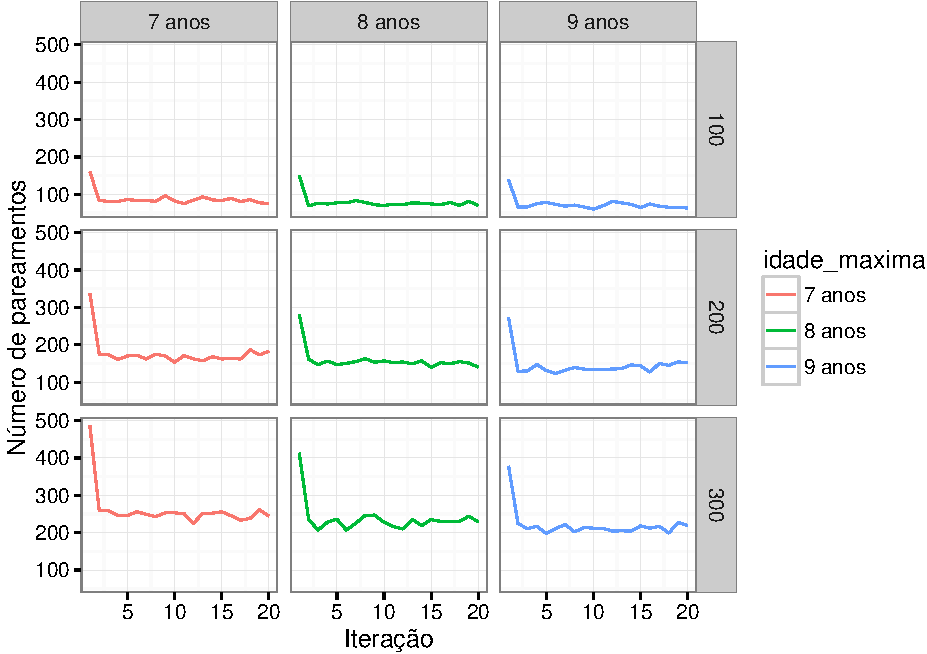
\includegraphics{curso-jurimetria_files/figure-latex/unnamed-chunk-78-1.pdf}

\subsubsection{Estratégia utilizada}\label{estrategia-utilizada}

O número de pareamentos certamente é invariante com relação à estratégia
utilizada, já que a diferença entre os dois métodos está apenas em qual
pretendente será escolhido.

Por outro lado, o número de crianças disponíveis pode diminuir conforme
pretendentes menos restritivos forem sendo preteridos. A figura abaixo
sugere que este efeito não é sentido. Isso deve-se, provavelmente, a
distância entre a idade máxima tolerada pelos pretendentes e as idades
das crianças cadastradas.

\begin{Shaded}
\begin{Highlighting}[]
\KeywordTok{expand.grid}\NormalTok{(}\DataTypeTok{tipo =} \DecValTok{1}\NormalTok{:}\DecValTok{2} \NormalTok{, }\DataTypeTok{K =} \KeywordTok{c}\NormalTok{(}\DecValTok{100}\NormalTok{,}\DecValTok{200}\NormalTok{,}\DecValTok{300}\NormalTok{)) %>%}\StringTok{    }\NormalTok{plyr:::}\KeywordTok{mdply}\NormalTok{(criancas_disponiveis, }\DataTypeTok{tempo =} \DecValTok{1}\NormalTok{:}\DecValTok{20}\NormalTok{) %>%}\StringTok{ }
\StringTok{  }\NormalTok{reshape2::}\KeywordTok{melt}\NormalTok{(}\DataTypeTok{id.vars =} \KeywordTok{c}\NormalTok{(}\StringTok{'tipo'}\NormalTok{,}\StringTok{'K'}\NormalTok{)) %>%}\StringTok{ }
\StringTok{  }\KeywordTok{select}\NormalTok{(-variable) %>%}\StringTok{ }
\StringTok{  }\KeywordTok{group_by}\NormalTok{(tipo, K) %>%}\StringTok{ }
\StringTok{  }\KeywordTok{mutate}\NormalTok{(}\DataTypeTok{periodo =} \DecValTok{1}\NormalTok{:}\KeywordTok{n}\NormalTok{()) %>%}
\StringTok{  }\KeywordTok{ungroup}\NormalTok{() %>%}\StringTok{ }
\StringTok{  }\KeywordTok{mutate}\NormalTok{(}\DataTypeTok{tipo =} \KeywordTok{factor}\NormalTok{(tipo)) %>%}\StringTok{ }
\StringTok{  }\KeywordTok{ggplot}\NormalTok{(}\KeywordTok{aes}\NormalTok{(}\DataTypeTok{x =} \NormalTok{periodo, }\DataTypeTok{y =} \NormalTok{value, }\DataTypeTok{fill =} \NormalTok{tipo, }\DataTypeTok{color =} \NormalTok{tipo))+}
\StringTok{  }\KeywordTok{geom_line}\NormalTok{()+}
\StringTok{    }\KeywordTok{facet_wrap}\NormalTok{(~K)+}
\StringTok{  }\KeywordTok{theme_bw}\NormalTok{()}
\end{Highlighting}
\end{Shaded}

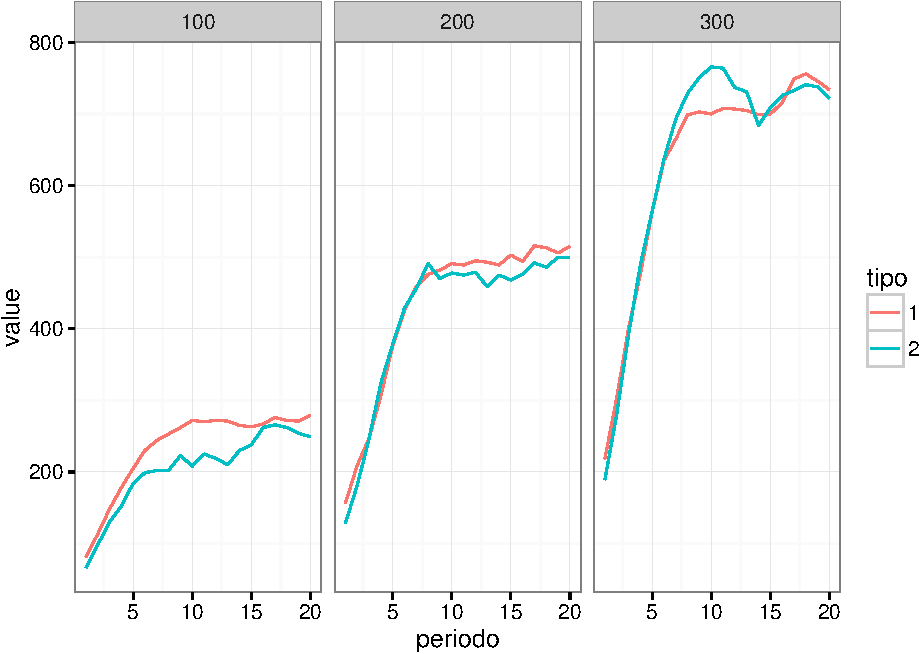
\includegraphics{curso-jurimetria_files/figure-latex/unnamed-chunk-79-1.pdf}

\begin{Shaded}
\begin{Highlighting}[]
\KeywordTok{expand.grid}\NormalTok{(}\DataTypeTok{tipo =} \DecValTok{1}\NormalTok{:}\DecValTok{2} \NormalTok{, }\DataTypeTok{K =} \KeywordTok{c}\NormalTok{(}\DecValTok{100}\NormalTok{,}\DecValTok{200}\NormalTok{,}\DecValTok{300}\NormalTok{)) %>%}\StringTok{    }\NormalTok{plyr:::}\KeywordTok{mdply}\NormalTok{(maiores_de_idade, }\DataTypeTok{tempo =} \DecValTok{1}\NormalTok{:}\DecValTok{20}\NormalTok{) %>%}\StringTok{ }
\StringTok{  }\NormalTok{reshape2::}\KeywordTok{melt}\NormalTok{(}\DataTypeTok{id.vars =} \KeywordTok{c}\NormalTok{(}\StringTok{'tipo'}\NormalTok{,}\StringTok{'K'}\NormalTok{)) %>%}\StringTok{ }
\StringTok{  }\KeywordTok{select}\NormalTok{(-variable) %>%}\StringTok{ }
\StringTok{  }\KeywordTok{group_by}\NormalTok{(tipo, K) %>%}\StringTok{ }
\StringTok{  }\KeywordTok{mutate}\NormalTok{(}\DataTypeTok{periodo =} \DecValTok{1}\NormalTok{:}\KeywordTok{n}\NormalTok{()) %>%}
\StringTok{  }\KeywordTok{ungroup}\NormalTok{() %>%}\StringTok{ }
\StringTok{  }\KeywordTok{mutate}\NormalTok{(}\DataTypeTok{tipo =} \KeywordTok{factor}\NormalTok{(tipo)) %>%}\StringTok{ }
\StringTok{  }\KeywordTok{ggplot}\NormalTok{(}\KeywordTok{aes}\NormalTok{(}\DataTypeTok{x =} \NormalTok{periodo, }\DataTypeTok{y =} \NormalTok{value, }\DataTypeTok{fill =} \NormalTok{tipo, }\DataTypeTok{color =} \NormalTok{tipo))+}
\StringTok{  }\KeywordTok{geom_line}\NormalTok{()+}
\StringTok{    }\KeywordTok{facet_wrap}\NormalTok{(~K)+}
\StringTok{  }\KeywordTok{theme_bw}\NormalTok{()}
\end{Highlighting}
\end{Shaded}

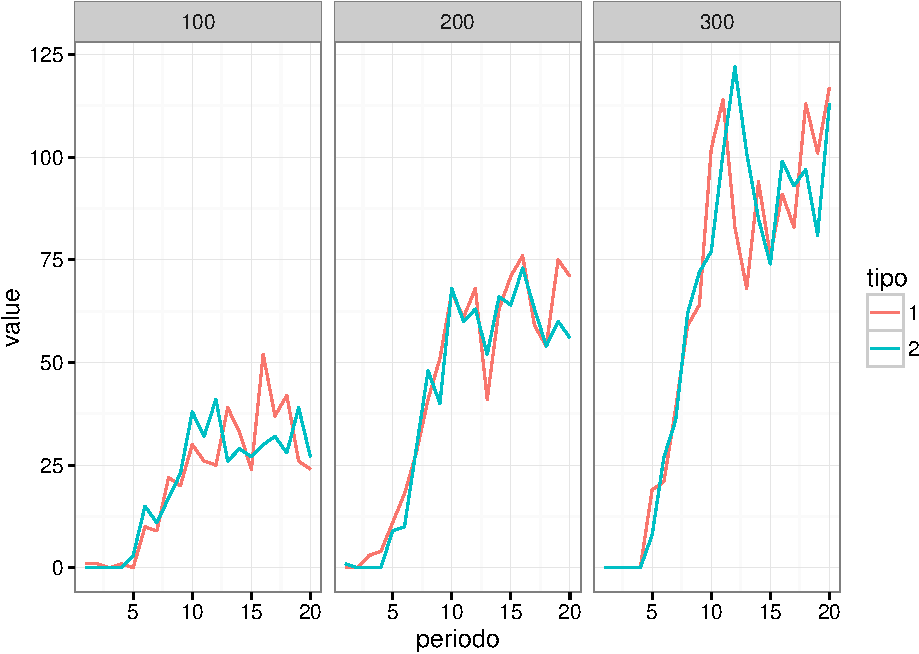
\includegraphics{curso-jurimetria_files/figure-latex/unnamed-chunk-79-2.pdf}

\chapter{Links}\label{links}

\textbf{Palestras}

Julio Trecenti:

\begin{itemize}
\tightlist
\item
  \href{http://rpubs.com/julio_trecenti/ferramental}{Ferramental da
  ABJ}.
\item
  \href{http://rpubs.com/julio_trecenti/scrape}{Web Scraping}.
\item
  \href{http://rpubs.com/julio_trecenti/adm}{Administração do
  judiciário}.
\end{itemize}

Fernando Correa:

\begin{itemize}
\tightlist
\item
  \href{https://github.com/abjur/curso/raw/master/pres/curso_tse.pdf}{Análise
  de sobrevivência}.
\item
  \href{https://github.com/abjur/alocTJSP}{Alocação de varas}.
\item
  \href{https://github.com/abjur/tjsp_app}{Waze}.
\end{itemize}

Rafael Stern:

\begin{itemize}
\tightlist
\item
  \href{https://github.com/abjur/curso/raw/master/pres/presentation-teoria-decisao.pdf}{Teoria
  da decisão (apresentação)}.
\item
  \href{https://github.com/abjur/curso/raw/master/pres/teoria_decisao.pdf}{Teoria
  da decisão (texto)}.
\item
  \href{https://github.com/abjur/curso/raw/master/pres/presentation_guidelines.pdf}{Weinstein}.
\item
  \href{https://github.com/abjur/curso/raw/master/pres/mining.pdf}{Topic
  Models}.
\end{itemize}

Carlos Alberto de Bragança Pereira:

\begin{itemize}
\tightlist
\item
  \href{https://github.com/abjur/curso/raw/master/pres/Aula_Brasilia.pdf}{Inferência
  Bayesiana e estatística forense}.
\item
  \href{https://github.com/abjur/curso/raw/master/pres/BAYESIAN_SCIENCE_FORENSIC_W.pdf}{Livro
  de estatística forense}.
\end{itemize}

Julio Michael Stern:

\begin{itemize}
\tightlist
\item
  \href{https://www.ime.usp.br/~jstern/miscellanea/jmsslide/ABJ161.pdf}{Intencionalidade
  vs Randomização}.
\end{itemize}

Adilson Simonis:

\begin{itemize}
\tightlist
\item
  \href{https://github.com/abjur/curso/raw/master/pres/conference_presentation(6).pdf}{Tópicos
  de probabilidade e estatística}.
\end{itemize}

\textbf{Outros links}

\begin{itemize}
\tightlist
\item
  Github da ABJ: \url{https://github.com/abjur}
\item
  Github do Julio: \url{https://github.com/jtrecenti}
\item
  Github do Fernando: \url{https://github.com/azeloc}
\item
  \href{http://www.somos.ufscar.br/professores/view/3477}{Página do
  Rafael Stern}
\end{itemize}

\chapter{Referências}\label{referencias}

ocite

Allen TT, Bernshteyn M (2008) Helping Franklin county vote in 2008:
Waiting line report to Michael Stinziano and Matthew Damschroder and The
Franklin County Board of Elections
\url{http://vote.franklincountyohio.gov/assets/pdf/press-releases/PR-07302008.pdf}

Karnon J, Stahl J, Brennan A, et al. Modeling using discrete event
simulation: a report of the ISPOR-SMDM Modeling Good Research Practices
Task Force---4. Med Decis Making. 2012; 32(5):701--11.

Dimitris Bertsimas and John N. Tsitsiklis (1997), Introduction to Linear
Optimization, Athena Scientific.

Alexey Izmailov and Mikhail Solodov (2007). Optimization, Volume 2:
Computational Methods. Rio de Janeiro, Brazil. Second Edition

\bibliography{packages.bib,book.bib}


\end{document}
